\documentclass[12pt, a4paper]{report}

\usepackage[utf8]{inputenc}
\usepackage{geometry}
 \geometry{
 a4paper,
 total={170mm,257mm},
 left=20mm,
 top=20mm,
}

\usepackage{titlesec}
\titleformat
{\chapter}
[display]{\bfseries\Large\itshape}
{Capitolo Nr.\thechapter}
{0.5ex}
{
    \rule{\textwidth}{1pt}
    \vspace{1ex}
	\centering
}
[\vspace{-0.5ex}\rule{\textwidth}{0.3pt}]

\renewcommand{\contentsname}{Indice}

\title{Dispense di Reti di calcolatori}
\author{Leonardo De Faveri}
\date{A.A. 2021/2022}

\usepackage[dvipsnames]{xcolor}
\usepackage{hyperref}
\hypersetup{
  colorlinks,
  linkcolor={red!90!black},
  citecolor={blue!50!black},
  urlcolor={blue!80!black}
  pdftitle={Dispense di reti di calcolatori},
  pdfpagemode=FullScreen,
}

\usepackage{graphicx}
\usepackage[export]{adjustbox}
\usepackage{subfig}
\usepackage{caption}
\graphicspath{{./images/}}% Imposta il percorso relativo per le immagini
\renewcommand{\figurename}{Fig.}% Cambia il testo delle caption

\usepackage{amssymb,amsmath,amsthm}
\theoremstyle{remark}
\newtheorem*{note}{\textbf{NB}}

\newtheoremstyle{def}
{\topsep}{\topsep}%
{\em}{}%
{\bfseries}{}
{\newline}
{%
  \rule{\textwidth}{0.4pt}\\*%
  \thmname{#1}~\thmnumber{#2}\thmnote{\ -\ #3}\label{def:#2}.\\*[-1.5ex]%
  \rule{\textwidth}{0.4pt}
}

\newtheoremstyle{eg}
{\topsep}{\topsep}%
{\em}{}%
{\bfseries}{}
{\newline}
{%
  \rule{\textwidth}{0.4pt}\\*%
  \thmname{#1}~\thmnumber{#2}\thmnote{\ -\ #3}\label{eg:#2}.\\*[-1.5ex]
  \rule{\textwidth}{0.4pt}
}

\theoremstyle{def}
\newtheorem{definition}{Definizione}
\theoremstyle{eg}
\newtheorem{eg}{Esempio}

\newtheoremstyle{codestyle}
{\topsep}{\topsep}%
{\tt\color{Sepia!90!Black}}{}%
{\bfseries\color{black}}{}
{\newline}
{%
  \rule{\textwidth}{0.4pt}\\*%
  \thmname{#1}~\thmnumber{#2}\thmnote{\ -\ #3}\label{code:#2}.\\*[-1.5ex]
  \rule{\textwidth}{0.4pt}
}
\theoremstyle{codestyle}
\newtheorem{codeblock}{Frammento}
\newenvironment{code}[1]
{\begin{codeblock}[#1]\hbadness=10000}{\end{codeblock}}
\newenvironment{minicode}[1]
{\begin{codeblock}[#1]\hbadness=10000\begin{minipage}[t]{\textwidth}}
{\end{minipage}\end{codeblock}}
\newenvironment{codecont}{\noindent\tt\color{Sepia!90!Black}\hbadness=10000}{}

\newcommand{\com}[1]{{\color{ForestGreen}\% #1}\\}
\newcommand{\bc}[1]{{\bf#1}}
\newcommand{\nl}{\par\smallskip\noindent}

\newcommand{\customindent}{19pt}
\newcommand{\lineheight}{\baselineskip}
\newcommand{\rmbreak}{\par\vspace{-\lineheight}}
\newcommand{\fstart}{\hspace{-\customindent}\par\rmbreak}
\newcommand{\ind}{\noindent\hangindent=\customindent}
\newcommand{\indf}{\rmbreak\hspace*{\customindent}\hangindent=38pt}
\newcommand{\indff}{\rmbreak\hspace*{38pt}\hangindent=57pt}
\newcommand{\indfff}{\rmbreak\hspace*{57pt}\hangindent=76pt}
\newcommand{\indffff}{\rmbreak\hspace*{76pt}\hangindent=95pt}
\newcommand{\indfffff}{\rmbreak\hspace*{95pt}\hangindent=114pt}

\usepackage[toc, automake]{glossaries}
\usepackage{glossary-mcols}
\setglossarystyle{mcolindexgroup}

\newglossary*{glos}{Glossario}
\newglossary*{prot}{Protocolli}
\makeglossaries
\loadglsentries{glossaries/glossario.tex}
\loadglsentries{glossaries/protocolli.tex}

\newcommand{\quotes}[1]{``#1''}
\newcommand{\hitem}[1]{\refstepcounter{enumii}\hypertarget{#1:\arabic{enumii}}{\item}}
\newcommand{\Mod}[1]{\ \mathrm{mod}\ #1}

\usepackage{numprint}
\usepackage{listings}
\usepackage[title]{appendix}
\usepackage{nameref}
\usepackage{bm}

\begin{document}
\maketitle
\tableofcontents

\chapter{Introduzione}
Nel corso di questa trattazione andremo ad affrontare i temi fondamentali nello
studio delle reti di calcolatori.

\section{Struttura di internet}
Parlando di reti, la prima cosa che viene in mente è certamente internet, la rete
per antonomasia. La rete internet, in realtà, non è una singola rete, ma è
definita come la \emph{rete di tutte le reti}.

Questo può far venire il sospetto che le reti di calcolatori siano strutture in
qualche modo. Infatti è così! Internet è organizzato in una struttura
gerarchica, al cui vertice, o nucleo, troviamo gli \emph{\gls{glos:ISP} di
livello 1}, al livello inferiore gli \emph{ISP di livello 2}, poi gli \emph{ISP
di livello 3} e per finire, al livello più basso, si collocano gli
\emph{\gls{glos:host}}, ovvero i \emph{dispositivi terminali} degli utenti.

Ma cosa sono gli \emph{ISP}? Un \emph{ISP} è un \emph{Internet Service Provider},
cioè una società o un ente che mette a disposizione l'infrastruttura necessaria
a comunicare con altri utenti della rete. Ma vediamone meglio le differenze:
\begin{enumerate}
    \item \emph{ISP di livello 1}: (Telecom, AT\&T, \dots) sono pochi enti
    distribuiti nel mondo, ma che hanno una copertura nazionale/internazionale.
    Sono fittamente interconnessi e comunicano come pari;
    \item \emph{ISP di livello 2}: (Vodafone, Tim, \dots) sono enti che si
    appoggiano all'infrastruttura di uno o più \emph{ISP di livello 1} e hanno
    una copertura distrettuale/nazionale. Possono comunicare soltanto con gli
    \emph{ISP} dei quali sfruttano l'infrastruttura;
    \item \emph{ISP di livello 3}: sono le cosiddette \emph{reti di ultimo
    salto} o \emph{reti di accesso} e permettono agli utenti finali di accedere
    alla rete e quindi hanno una copertura locale;
\end{enumerate}

\paragraph{Internet Exchange Point}
Gli \emph{ISP di livello 2} possono comunicare direttamente tra loro, senza scalare
la gerarchia, attraverso punti particolari della rete detti \emph{\gls{glos:IXP}},
\emph{Internet Exchange Point}. Questi sono luoghi in cui le infrastrutture di
due o più \emph{ISP di livello 2} sono messe in comunicazione, permettendo così
al traffico dati di passare da un'infrastruttura all'altra. Questo tipo di
interscambi consentono, come vedremo, di ridurre il tempo necessario per il
trasferimento dei dati.

\paragraph{Reti single-homed e multi-homed}
Gli \emph{ISP di livello 3} possono appoggiarsi a uno o più \emph{ISP di livello
di 2}. Nel primo caso configurano una \emph{single-homed network}, mentre nel
secondo una \emph{multi-homed network}.

\subsection{Nucleo della rete}
La struttura gerarchica appena descritta permette di distinguere due livelli
della rete: un \emph{nucleo} e una \emph{periferia}.

Il \emph{nucleo} corrisponde alla parte di rete gestita dagli \emph{ISP di livello
1 e 2}, cioè la parte di infrastruttura non direttamente accessibile dagli utenti.
È evidente che questa parte della rete è quella in cui circola la maggior parte
del traffico, per cui rallentamenti, congestioni e guasti hanno conseguenze più
gravi. Per questo motivo, i dispositivi fisici che compongono
l'infrastruttura, oltre che essere più performanti delle loro controparti di
\emph{periferia}, sono collegati tramite strutture magliate. Ciò significa che
tra due dispositivi esistono una pluralità di collegamenti e percorsi possibili.
Questa ridondanza permette di ridurre il rischio di interruzioni del servizio, ma
anche di distribuire il traffico in maniera più efficiente, evitando che si
concentri su un unico punto.

\subsection{Periferia della rete}
La parte \emph{periferica} di internet corrisponde alla somma delle
\emph{reti di accesso}, cioè alla parte di competenza degli \emph{ISP di livello
3}. Questa parte della rete funge da interfaccia di collegamento per gli utenti
e i dispositivi terminali, cioè inoltra verso il \emph{nucleo} i dati da
trasmettere e riceve i dati in arrivo per poi occuparsi di farli arrivare
all'\emph{host} o al gruppo di \emph{host} destinatari.

Esistono diversi tipi di \emph{reti d'accesso} che si distinguono per la
dimensione e le tecnologie utilizzate.
Dividendole per dimensione si hanno:
\begin{itemize}
    \item \emph{Reti d'accesso residenziali}: coprono l'area di un'abitazione;
    \item \emph{Reti d'accesso aziendali}: coprono l'area di più edifici, o di
    un campus;
\end{itemize}

\noindent
Suddividendole invece per tecnologia si hanno:
\begin{itemize}
    \item \emph{Reti d'accesso punto-punto}: i dispositivi sono connessi
    direttamente, o attraverso uno \emph{\gls{glos:switch}} al 
    \emph{\gls{glos:router}}. È possibile un'ulteriore suddivisione:
    \begin{itemize}
        \item \emph{Reti con modem dial-up}: è una tecnologia vecchia e lenta
        che sfrutta i collegamenti telefonici in maniera esclusiva, cioè non
        permette di telefonare e accedere alla rete in contemporanea;
        \item \emph{Reti \gls{glos:DSL}}: sfrutta anch'essa i collegamenti
        telefonici, ma non in modo esclusivo;
        \item \emph{Reti \gls{glos:FTTH}}: il \emph{router} locale è connesso
        all'\emph{ISP di livello 2} tramite collegamenti in \emph{fibra ottica}
        molto veloci;
    \end{itemize}
    \item \emph{Reti d'accesso wireless}: usano tecnologie wireless e tanti utenti
    si connettono allo stesso punto, detto \emph{base station} o \emph{access point},
    il quale è connesso a un \emph{router};
\end{itemize}

\section{Mezzi trasmissivi}
All'interno delle reti, le informazioni, codificate in bit, viaggiano su dei
\emph{mezzi trasmissivi}. Ne esistono di tipologie diverse:
\begin{itemize}
    \item \emph{Mezzi guidati}: i segnali si propagano su un mezzo \emph{fisico}
    \begin{itemize}
        \item \emph{Doppini intrecciati}: è un cavo costituito da due fili di rame
        intrecciati;
        \item \emph{Cavi coassiali}: è un cavo costituito da un'anima centrale di
        rame e una maglia costituita da cavi metallici intrecciati. L'anima e la
        maglia sono separati da uno strato isolante;
        \item \emph{Fibra ottica}: l'informazione viaggia sotto forma di impulsi
        luminosi e questa è la soluzione ottimale per le lunghe distanze;
    \end{itemize}
    \item \emph{Mezzi a onda libera}: i segnali si propagano attraverso l'atmosfera
    e lo spazio esterno sfruttando i campi elettromagnetici
    \begin{itemize}
        \item \emph{Reti a microonde terrestri};
        \item \emph{Reti Wi-Fi}: le più usate nelle \emph{reti locali};
        \item \emph{Reti cellulari}: le più usate per la mobilità;
        \item \emph{Reti satellitari}: sono ottimali per le lunghe distanze e per
        luoghi che non hanno accesso a \emph{reti cellulari};
    \end{itemize}
\end{itemize}
I \emph{mezzi a onda libera} esaltano la mobilità, in quanto non è richiesto un
collegamento fisico con il punto d'accesso alla rete, ma sono maggiormente soggetti
a problemi di interferenze e riflessioni dei segnali. Per i \emph{mezzi guidati}
vale il contrario.

\subsection{Doppini intrecciati}
Esaminiamo più a fondo i \emph{doppini intrecciati} che sono quelli tipicamente
usati nello standard \emph{Ethernet}. Un cavo di questo tipo è formato da 4
coppie di fili di rame intrecciati detti \emph{doppini}.

Per evitare problemi di interferenza tra i cavi o i singoli \emph{doppini} è
possibile usare delle schermature. Diverse configurazione delle schermature sono
codificate con un sistema di lettere:
\[X/YTP\]
dove $X$ indica il tipo di schermatura del cavo e $Y$ la schermatura dei singoli
doppini.
\newline Schermatura del cavo:
\begin{itemize}
    \item \emph{U}: unshilded;
    \item \emph{F}: foiled (rivestito con una lamina di alluminio);
    \item \emph{S}: rivestito con una maglia metallica (rame placcato in alluminio);
    \item \emph{SF}: entrambe;
\end{itemize}
Schermatura dei \emph{doppini};
\begin{itemize}
    \item \emph{U}: unshilded;
    \item \emph{F}: shielded;
\end{itemize}

\paragraph{Cavi patch VS cavi cross}
Nello standard \emph{Ethernet}, nelle prese \emph{RJ45}, i 4 \emph{doppini} sono
collegati ai pin della presa mettendoli in riga affiancati. Nei \emph{cavi patch}
l'ordine dei \emph{doppini} è uguale a entrambi i capi del cavo, mentre nei cavi
\emph{cross} i due \emph{doppini} esterni sono scambiati di posizione e allo
stesso modo sono scambiati anche i \emph{doppini} interni.

\section{Tecniche di commutazione}
Abbiamo detto come i bit di dati viaggino da un dispositivo a un altro, ma non
abbiamo ancora chiarito come siano organizzati questi trasferimenti. Ciò è definito
dalla \emph{tecnica di commutazione} utilizzata. Ne esistono due:
\begin{itemize}
    \item \emph{Commutazione di circuito}: prima del trasferimento viene stabilito
    a priori il percorso che il messaggio dovrà seguire;
    \item \emph{Commutazione a pacchetto}: il messaggio viene scomposto in pacchetti
    che attraversano la rete in modo indipendente gli uni dagli altri;
\end{itemize}

\subsection{Commutazione di circuito}
Come accennato, questa \emph{tecnica di commutazione} prevede che il messaggio
venga trasmesso in blocco e che le risorse necessarie a collegare mittente e
destinatario siano riservate per quella comunicazione.

Ad essere suddivisa in porzioni è l'\emph{ampiezza di banda} (il \emph{bandwidth})
secondo 3 parametri:
\begin{enumerate}
    \item \emph{Bit rate}: e.g. in una rete a $10\frac{Mb}{s}$ vengono creati due
    canali da $5\frac{Mb}{s}$ che vengono assegnati a due utenti senza un limite
    di tempo;
    \item \emph{Frequenza}: (\emph{\gls{glos:FDM}}) la frequenza
    viene suddivisa in più canali che vengono assegnati agli utenti senza un limite
    di tempo;
    \item \emph{Tempo}: (\emph{\gls{glos:TDM}}) ogni utente ha a
    disposizione per un tempo limitato tutta la frequenza del canale;
\end{enumerate}

\begin{figure}[h]
    \centering
    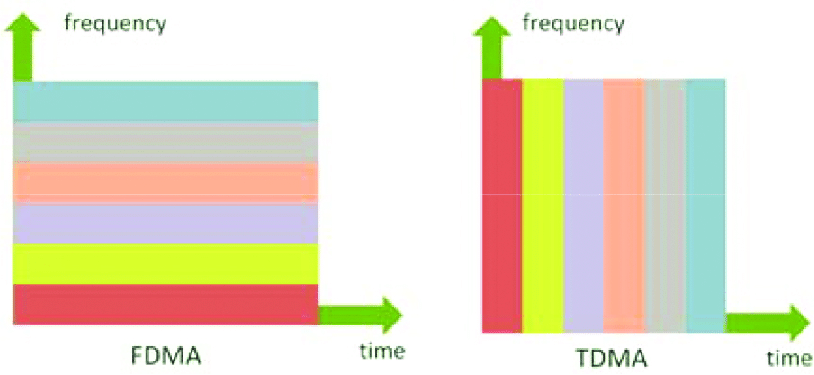
\includegraphics[width=\textwidth]{images/fdm-tdm.png}
    \caption{\emph{FDM} VS \emph{TDM}}
\end{figure}\noindent
Il vantaggio di questo tipo di \emph{commutazione} è che ogni utente al quale è
stato assegnato un canale (o slot) sa quali risorse avrà a disposizione. Tuttavia,
queste risorse devono essere negoziate prima della trasmissione e quindi è prevista
una fase di \emph{handshake} nella quale vengono prenotate e assegnate le risorse.
Inoltre, quando l'utente non le usa, quelle risorse sono sprecate.

\subsection{Commutazione a pacchetto}
Diversamente da prima, qui il messaggio viene suddiviso in pacchetti di uguale
dimensione (tipicamente 1.5MB) che vengono trasmessi singolarmente. Nel momento
della trasmissione, il pacchetto utilizza tutta la banda del canale che non viene
quindi ripartita tra gli utenti, ma condivisa. In questo modo, l'uso delle
risorse avviene a seconda delle necessità e, infatti, questa \emph{tecnica di
commutazione} è adatta per situazioni in cui un utente utilizza la rete soltanto
per pochi istanti.

Questa tecnica è soggetta a problemi di \emph{congestione} provocata dall'accodamento
dei pacchetti in attesa di essere trasmessi e ciò è anche diretta conseguenza
del comportamento dei commutatori. I commutatori infatti, prima di trasmettere un
pacchetto devono riceverlo per intero. Per questo motivo in ogni commutatore esiste
un buffer nel quale vengono memorizzati i pacchetti in attesa di essere
trasmessi e, quando questo è pieno, i nuovi pacchetti in arrivo vengono scartati.

Questo problema di perdita dei pacchetti viene risolto (se serve!) da determinati
protocolli che verranno trattati più avanti.

\paragraph{Ritardi nelle trasmissioni}
Nella comunicazione in rete, specie con la \emph{commutazione a pacchetto},
\emph{ritardi e perdite} sono eventi molto frequenti. Il problema delle
\emph{perdite} è già stato discusso. Vediamo quindi quali sono le cause dei
\emph{ritardi}:
\begin{itemize}
    \item \emph{Ritardo di elaborazione del nodo}: il nodo richiede tempo per
    controllare la correttezza dei dati e per determinare il canale attraverso il
    quale trasmettere il pacchetto;
    \item \emph{Ritardo di accodamento}: i pacchetti che devono essere inviati
    vengono inseriti in un buffer e in caso di congestione gli ultimi pacchetti
    possono dover attendere a lungo prima di essere trasmessi;
    \item \emph{Ritardo di trasmissione}: dipende rapporto tra la dimensione in
    \emph{bit} del pacchetto ($L$) e la \emph{frequenza di trasmissione} in
    $bit/s$ del collegamento ($R$), cioè $L/R$;
    \item \emph{Ritardo di propagazione}: dipende dal rapporto tra la
    \emph{lunghezza} ($d$) e la \emph{velocità di propagazione} ($s$) del
    collegamento fisico, cioè $d/s$;
\end{itemize}

\begin{note}
    Sebbene possano sembrare simili, $R$ e $s$ sono in realtà due grandezze molto
    differenti! $R$ è espressa in $bit/s$, mentre $s$ in $m/s$ e tipicamente vale
    circa $2\cdot 10^8m/s$.
\end{note}\noindent
Il ritardo totale su un nodo è dato quindi dalla somma di tutti questi fattori:
\[d_{nodo}=d_{proc}+d_{accodamento}+d_{trasferimento}+d_{propagazione}\]
Da qui, possiamo definire il concetto di \emph{throughput}:
\begin{definition}[Throughput]
    È definito throughput la frequenza, espressa in \emph{dati/unità di tempo},
    alla quale una certa unità di dati viene trasferita tra mittente e destinatario.
\end{definition}

\section{Protocolli di comunicazione}
Alla fine del paragrafo precedenti abbiamo accennato ai \emph{protocolli di
comunicazione}. Diamone qui una prima definizione:

\begin{definition}[Protocollo]
    Un protocollo definisce il formato e l'ordine dei messaggi scambiati
    fra due o più entità in comunicazione.
\end{definition}\noindent
Esistono una gran varietà di protocolli e sono organizzati in uno \emph{stack}
detto \emph{stack protocollare}. Esistono due principali \emph{stack protocollari}:
lo \emph{Stack TCP/IP} e il \emph{Modello ISO/OSI}.

La differenza tra i due è che il \emph{modello ISO/OSI} è semplicemente un modello
di riferimento per la definizione di altri \emph{stack}, mentre il \emph{TCP/IP} è
lo \emph{stack} usato nelle comunicazioni in internet.

\begin{figure}[h]
    \centering
    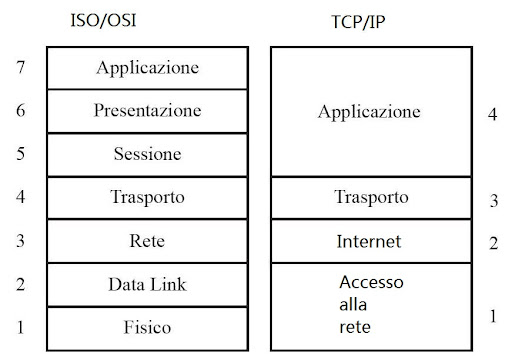
\includegraphics[scale=0.6]{stack-protocollari-a-confronto.jpg}
    \caption{\emph{ISO/OSI} VS \emph{TCP/IP}}
\end{figure}

\paragraph{Livelli dello stack protocollare ISO/OSI}
Esaminiamo il significato dei vari livelli dello stack \emph{ISO/OSI}:
\begin{enumerate}
    \item \emph{Fisico}: gestisce il trasferimento dei singoli bit
    \item \emph{Data link}: organizza l'instradamento dei frame attraverso una serie
    di commutatori;
    \item \emph{Rete}: instrada i pacchetti verso la rete del destinatario;
    \item \emph{Trasporto}: gestisce l'instradamento dei segmenti verso una
    specifica applicazione attiva nella rete di destinazione;
    \item \emph{Sessione}: gestisce sessioni di comunicazioni e la sincronizzazione
    dei flussi di dati (e.g. streaming audio-video);
    \item \emph{Presentazione}: consente alle applicazioni di interpretare il
    significato dei dati gestendo parametri come compressione e cifratura;
    \item \emph{Applicazione}: fornisce alle applicazioni i mezzi per scambiarsi
    messaggi;
\end{enumerate}
Il motivo per cui nello \emph{stack TCP/IP} mancano i livelli \emph{sessione} e
\emph{presentazione} è che possono essere inclusi nei protocolli di
\emph{livello Applicazione};

\paragraph{Incapsulamento}
La stratificazione dei protocolli consente di rendere modulare la comunicazione in
rete. La modularità porta numerosi vantaggi, tra i quali:
\begin{itemize}
    \item \emph{Trasparenza}: una modifica ai protocolli di un livello è trasparente
    ai protocolli di altri livelli;
    \item \emph{Semplificazione}: il modello a strati permette di identificare più
    facilmente i diversi componenti di un sistema che altrimenti risulterebbe
    estremamente complesso;
\end{itemize}

\paragraph{Comunicazione tra livelli}
Ogni \emph{livello} (\emph{layer}) fornisce un servizio al \emph{livello}
superiore, il quale vede il \emph{livello} inferiore come una black-box della
quale sfruttarne i servizi.

\begin{figure}[h]
    \centering
    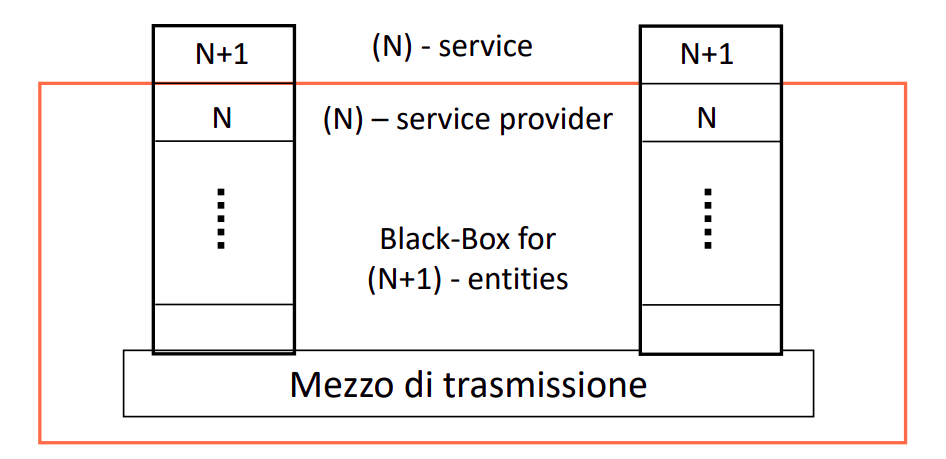
\includegraphics[width=\textwidth]{modularizzazione-protocolli.png}
    \caption{Modularizzazione dei servizi}
\end{figure}\noindent
La comunicazione tra livelli avviene mediante \emph{\gls{glos:SAP}}, in
modo che un servizio del \emph{livello N} è offerto all'entità di
\emph{livello N+1} attraverso un'interfaccia di programmazione detta
appunto \emph{SAP}. Lo scambio di informazioni tra entità dello stesso
\emph{livello}, invece, è regolata dai \emph{protocolli}.

\begin{figure}[h]
    \centering
    \subfloat[\emph{Comunicazione tra servizi di diverso livello}]{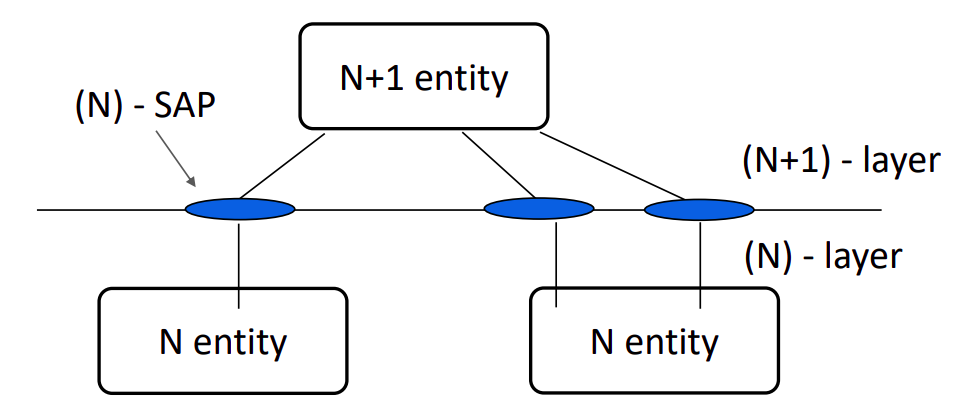
\includegraphics[scale=0.25]{comunicazione-servizi-diverso-livello.png}}
    \hfill
    \subfloat[\emph{Comunicazione tra servizi dello stesso livello}]{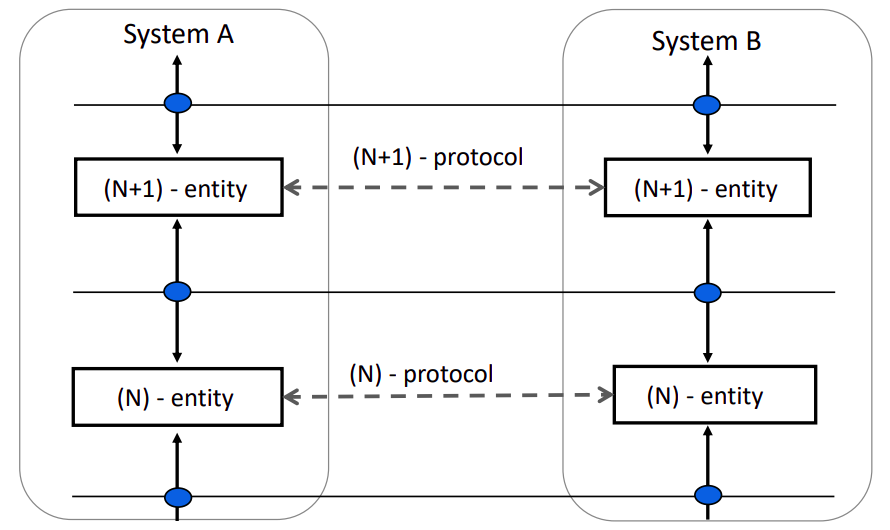
\includegraphics[scale=0.25]{comunicazione-servizi-stesso-livello.png}}
    \caption{Comunicazioni tra servizi}
\end{figure}

\paragraph{Data unit}
La suddivisione in livelli dei servizi cambia il modo in cui i dati, o meglio le
\emph{\gls{glos:DU}} da trasmettere vengono trattate. In un sistema a livelli, i dati da trasmettere da un \emph{livello
N} costituiscono un \emph{N-\gls{glos:SDU}} (\emph{SDU} di \emph{livello N}).

A questo \emph{N-SDU} il \emph{livello} aggancia il proprio \emph{N-\gls{glos:PCI}}
(\emph{PCI} di \emph{livello N}), cioè aggiunge le informazioni necessarie al
\emph{protocollo} per funzionare. Il risultato è un \emph{N-\gls{glos:PDU}}
(\emph{PDU} di \emph{livello N}).

Ogni \emph{livello} considera il \emph{PDU} del livello superiore come una busta
chiusa. Cioè, l'\emph{N-PDU} è l'\emph{SDU} di \emph{livello N-1} e aggiungendo
l'\emph{(N-1)-PCI} all'\emph{(N-1)-SDU} si ottiene l'\emph{(N-1)-PDU}.

\paragraph{Trasmissione e ricezione}
Nel momento della trasmissione i dati veri e propri vengono progressivamente
imbustati insieme al \emph{PCI} di livello, partendo dal \emph{livello Applicativo}
e scendendo fino al \emph{Fisico}. Per la ricezione, invece, si segue il processo
inverso, quindi partendo dal \emph{Fisico} e salendo all'\emph{Applicativo} ogni
\emph{livello} rimuove il proprio \emph{PCI}.

\begin{figure}[h]
    \centering
    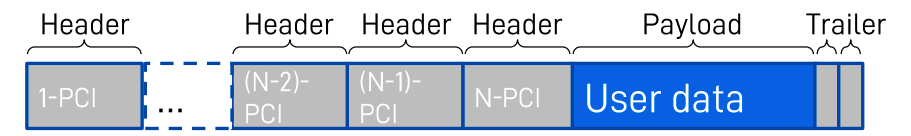
\includegraphics[width=\textwidth]{schema-di-un-PDU.png}
    \caption{Rappresentazione di un \emph{PDU} alla fine del processo di imbustamento}
\end{figure}\noindent
Le \emph{DU} possono essere:
\begin{itemize}
    \item \emph{Segmentate}: se la dimensione dei dati eccede il limite massimo,
    possono essere suddivisi in più \emph{SDU};
    \item \emph{Assemblate}: per evitare inefficienze, più \emph{N-SDU} di piccola
    dimensione possono essere aggregate in un unico \emph{N-SDU} e trasmesse insieme;
    \item \emph{Ri-assemblate}: è il processo inverso della \emph{segmentazione};
\end{itemize}

\paragraph{Le PDU di livello}
A seconda del \emph{livello} in cui si trovano le \emph{PDU} possono avere nomi
diversi:
\begin{itemize}
    \item \emph{Applicazione}: messaggi;
    \item \emph{Trasporto}: segmenti;
    \item \emph{Rete}: pacchetti;
    \item \emph{Data link}: frame;
\end{itemize}
\chapter{Livello Applicativo}
Il \emph{livello Applicativo} è l’ultimo livello dello \emph{stack protocollare TCP/IP}
e costituisce un’interfaccia per i processi che intendono comunicare sulla rete.

Vediamo più nel dettaglio le caratteristiche e le funzionalità, o meglio i
\emph{protocolli}, forniti da questo livello.

\section{Applicazioni di rete}
Uno degli utilizzi più diffusi della rete è la creazione di \emph{applicazioni di
rete}, ovvero applicazioni software diffuse su più calcolatori.

\subsection{Architetture di applicazioni di rete}
Le \emph{applicazioni di rete} possono essere basate su architetture diverse:
\begin{itemize}
    \item \emph{Client-server}: esistono \emph{server} che offrono servizi ad
    altri \emph{host} detti \emph{client}. I \emph{client} possono
    comunicare soltanto con i \emph{server};
    \item \emph{\gls{glos:P2P}}: non esistono \emph{server}, ma tutti gli
    \emph{host} sono pari tra loro. Ciascun \emph{host}, o \emph{peer}, può
    comunicare con qualsiasi altro \emph{peer};
    \item \emph{Architetture ibride}: sono architetture che hanno sia componenti
    \emph{client-server} che \emph{peer-to-peer};
    \item \emph{Cloud computing}: le risorse sono distribuite su uno o più server
    dislocati nel territorio e sono virtualizzate in modo che ogni utente
    possa utilizzare solo le risorse di cui ha bisogno;
\end{itemize}
Ma vediamole più nel dettaglio.

\paragraph{Architettura client-server}
Nelle reti basate sul modello \emph{Client-Server}, esiste un \emph{server}
centrale al quale molti \emph{client} si connettono per richiedere una risorsa o
usufruire di un servizio. Il \emph{server} deve essere sempre attivo e avere un
\emph{indirizzo IP} fisso, così da essere raggiungibile dai \emph{client}, i
quali, possono comunicare solo con lui e non tra loro.

\bigskip\noindent
Esistono quindi 2 entità:
\begin{itemize}
    \item \emph{Client}: si tratta di un componente hardware o software che invia
    delle richieste al \emph{server} e attende che questo risponda per poterne
    elaborare la risposta;
    \item \emph{Server}: si occupa di soddisfare le richieste ricevute dai
    \emph{client} e di restituire loro il risultato delle suddette richieste;
\end{itemize}
Tale modello ha come principale vantaggio la semplicità di gestione delle risorse
condivise, che risiedono tutte nel \emph{server}. Inoltre, permette di ridurre i
costi lato \emph{client} perché non è necessario che questi abbiano prestazioni
elevate. Tuttavia, nel caso di guasti o malfunzionamenti del \emph{server},
l’intera rete potrebbe risultare rallentata o inutilizzabile.

\begin{figure}[h]
    \centering
    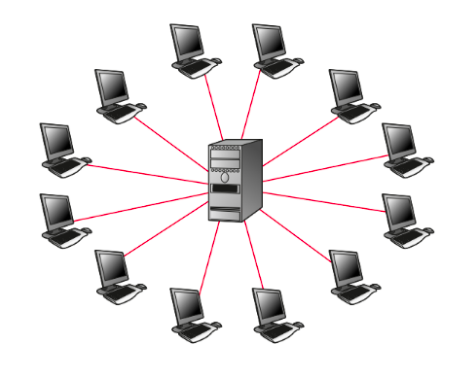
\includegraphics[width=0.4\textwidth]{modello-client-server.png}
    \caption{Schema architettura \emph{client-server}}
\end{figure}

\paragraph{Architettura P2P}
Il modello \emph{P2P} prevede la presenza di entità autonome dette \emph{peer}
che scambiano tra di loro delle risorse. Ogni \emph{peer} può sia condividere
risorse che richiederne.

Esistono diversi tipi di architetture \emph{P2P}:
\begin{itemize}
    \item \emph{P2P decentralizzato}: ogni \emph{peer} svolge sia la funzione di
    server che di client. Il sistema è in grado di adattarsi autonomamente a un
    cambiamento nei nodi partecipanti senza richiedere interventi esterni e
    mantenendo attiva la rete;
    \item \emph{P2P centralizzato}: Esiste un server centrale detto
    \emph{directory server} che contiene informazioni utili alla localizzazione
    delle risorse tra i \emph{peer}. Ogni \emph{peer} informa il server del
    tipo di risorse che intende condividere, mentre, quando ne richiede una,
    chiede al \emph{directory server} di localizzarla;
    \item \emph{P2P ibrido}: Esistono alcuni \emph{peer} detti \emph{super-peer},
    \emph{super-nodi} o \emph{ultra-peer} determinati dinamicamente da un algoritmo
    e che forniscono informazioni sulla localizzazione delle risorse agli altri
    \emph{peer}, detti \emph{leaf-peer};
\end{itemize}

\begin{figure}[h]
    \centering
    \subfloat[\emph{P2P decentralizzato}]{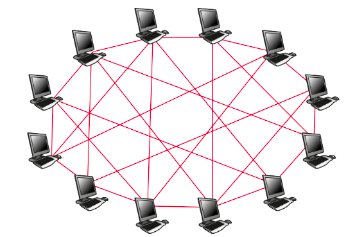
\includegraphics[scale=0.40]{modello-p2p-decentralizzato.png}}
    \hfill
    \subfloat[\emph{P2P centralizzato}]{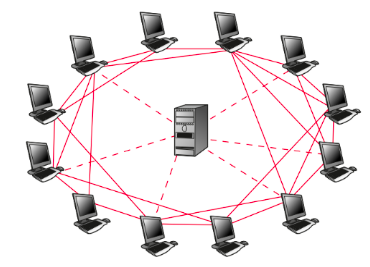
\includegraphics[scale=0.40]{modello-p2p-centralizzato.png}}
    \hfill
    \subfloat[\emph{P2P ibrido}]{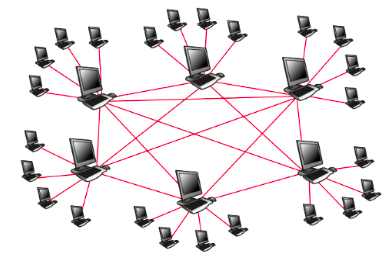
\includegraphics[scale=0.40]{modello-p2p-ibrido.png}}
    \caption{Architetture \emph{P2P} a confronto}
\end{figure}

\paragraph{Cloud computing}
Il \emph{cloud computing} è un insieme di risorse IT (hardware e software)
distribuite e accessibili attraverso la rete. In particolare, questa architettura
viene implementata come un \emph{sistema distribuito}, su diversi server dislocati
nel mondo, che vengono utilizzati per fornire un servizio.

Per accedere alle risorse i client contattano un \emph{endpoint}, cioè un server
che funge da interfaccia e che si occupa di recuperare le risorse
richieste contattando gli altri server della rete.

Questo modello porta con sé numerosi vantaggi:
\begin{itemize}
    \item \emph{Scalabilità}: è possibile aumentare o diminuire le risorse in
    base alle necessità;
    \item \emph{Velocità di configurazione}: attivare, modificare o
    disattivare un servizio è immediato;
    \item \emph{Risparmio per l'utilizzatore}: il costo varia in base all’utilizzo
    effettivo delle risorse, le quali, sono assegnate dinamicamente dal gestore
    con un sistema di \emph{provisioning dinamico} e con granularità fine;
    \item \emph{Risparmio per il fornitore}: le risorse sono virtualizzate,
    ovvero condivise tra tutti gli utilizzatori. Ciò implica che il sistema può
    avere a disposizione meno risorse di quelle che servirebbero a soddisfare le
    richieste dei client se queste venissero fatte tutte contemporaneamente (è un
    evento raro);
    \item \emph{Affidabilità}: eventuali disservizi sono risolti dal gestore e
    non dall'utilizzatore;
\end{itemize}
Ma ci sono anche delle criticità:
\begin{itemize}
    \item \emph{Sicurezza e privacy}: più utenti accedono allo stesso server per
    diverse ragioni, per cui è necessario assicurare che le attività di un utente
    non interferiscano con i dati o i processi degli altri;
    \item \emph{Problemi internazionali di natura economica e politica}: uno stato
    potrebbe decidere di impedire l'accesso ad un certo servizio offerto da un
    ente estero (e.g. servizi di Google non accessibili in Cina);
    \item \emph{Continuità del servizio offerto}: i fornitori di servizi devono
    garantire agli utenti la continua fruibilità dei propri servizi;
    \item \emph{Difficoltà di migrazione dei dati}: su un server risiedono molti
    dati per cui è complicato trasferirli da un'altra parte;
\end{itemize}
\begin{note}
    Quando si parla di \emph{scalabilità} è possibile distinguere due casi:
    \begin{itemize}
        \item \emph{Scalabilità orizzontale}: aggiungere nodi fornitori (server)
        alla rete;
        \item \emph{Scalabilità verticale}: incrementare le risorse di un singolo
        nodo;
    \end{itemize}
    Nel caso del \emph{cloud computing} viene esaltata la \emph{scalabilità
    orizzontale}.
\end{note}

\paragraph{Data center}
I fornitori di servizi cloud, dovendo gestire molti server, si appoggiano a
strutture attrezzate dove sono allocati i server di uno o più fornitori. Queste
strutture sono dette \emph{data center} e si occupano di garantire che i server
funzionino anche in caso di problemi quali, ad esempio, blackout o incendi.

\begin{figure}[ht]
    \centering
    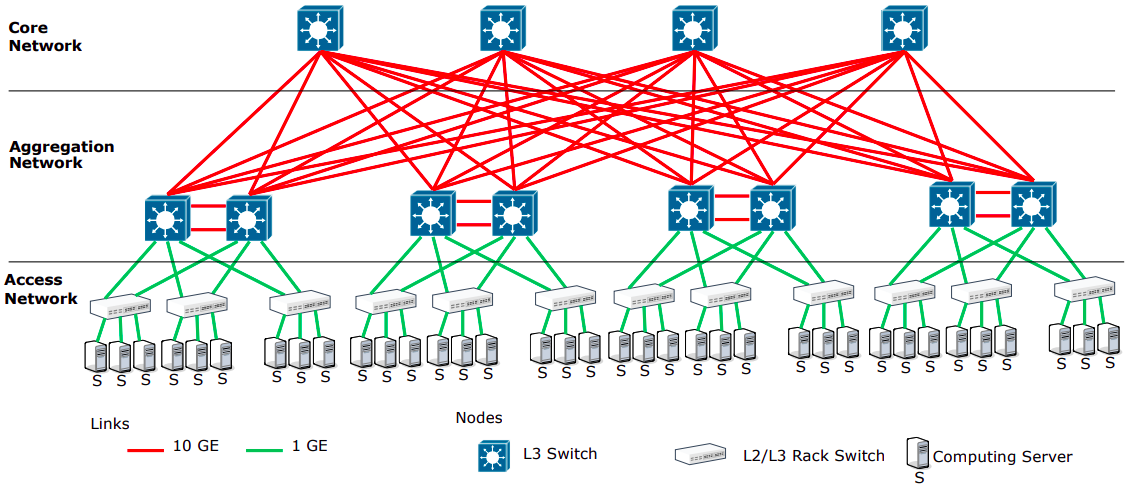
\includegraphics[width=\textwidth]{rete-data-center.png}
    \caption{Schema architetturale di un \emph{data center}}
\end{figure}
La figura sottostante mostra la struttura gerarchica della rete interna di un
\emph{data center}. In particolare, ogni server è collegato ad una rete
d'accesso; le reti d'accesso sono poi collegate ad una rete intermedia che aggrega
le comunicazioni provenienti dai server e le dirige verso la parte interna della
rete.

\paragraph{Content Delivery Network}
La struttura interna di un \emph{data center} può essere paragonata alla
struttura organizzativa dei server di grandi aziende IT come Google. Google ha 14
\emph{\quotes{mega-data center}} (\numprint{100000} server per \emph{data center})
distribuiti nel mondo che servono contenuti dinamici e personalizzati (e.g. gmail,
ricerche), 50 cluster (100-500 server per cluster) di calcolo
\emph{\quotes{bring home}} nelle reti degli \emph{IXP} che servono contenuti
statici (e.g. video di Youtube) e centinaia di cluster (decine di server per cluster)
\emph{\quotes{enter deep}} nelle reti degli \emph{ISP} che forniscono contenuti
statici (e.g. parti statiche nelle pagine dei risultati di ricerca) e permettono
il \emph{TCP splitting}.

Un'organizzazione di questo tipo permette la realizzazione di \emph{\gls{glos:CDN}},
reti \emph{\quotes{overlay}} per la diffusione di contenuti. L'idea alla base
delle \emph{CDN} è di portare i contenuti il più vicino possibile all'utente
finale in modo da ridurre la latenza, evitare colli di bottiglia e migliorare le
prestazioni generali della rete.

Esistono due tecniche per la realizzazione di \emph{CDN}:
\begin{itemize}
    \item \emph{Enter deep}: vengono installati server fisici nelle reti degli
    \emph{ISP} riducendo il ritardo e migliorando il \emph{throughput} percepito
    dagli utenti;
    \item \emph{Bring home}: vengono istallati server fisici nelle reti degli
    \emph{IXP} così da poter servire più \emph{ISP} contemporaneamente;
\end{itemize}

\section{Comunicazione in rete tra processi}
La comunicazione tra utenti si realizza come comunicazione tra processi, ovvero
programmi in esecuzione su un \emph{host}. Processi che comunicano tra loro sullo
stesso \emph{host} usano \emph{schemi interprocesso} definiti dal sistema
operativo. Quando, invece, a comunicare sono processi su \emph{host} diversi, lo
fanno mediante lo scambio di messaggi sulla rete.

Nella comunicazione in rete distinguiamo due tipi di processi:
\begin{itemize}
    \item \emph{Processi server}: forniscono un servizio e attendono di essere
    contatati da altri processi,
    \item \emph{Processi client}: usufruiscono di uno o più servizi richiedendoli
    a uno o più \emph{processi server}.
\end{itemize}

\begin{note}
    Nelle \emph{architetture P2P} le applicazioni hanno sia \emph{processi
    server} che \emph{processi client}.
\end{note}\noindent
Per realizzare la comunicazione in rete tra processi, questi devono poter essere
identificati all'interno della rete. Per farlo, è necessario conoscere gli
\emph{indirizzi IP} (indirizzi del \emph{livello Rete}) e i \emph{numeri di porta} dei
processi (indirizzi del \emph{livello Trasporto}) e questa coppia di parametri è
detta \emph{socket}.

\subsection{Socket}
\begin{definition}[Socket]
    Una socket è un'interfacci di un host, creata da un'applicazione
    e controllata dal Sistema Operativo, tramite la quale un processo di
    quell'applicazione può scambiare messaggi con il processo di un'altra
    applicazione.
\end{definition}\noindent
Le \emph{socket} sono basate sull'architettura \emph{client-server} quindi
esistono \emph{socket client} e \emph{socket server}.

La creazione e l'utilizzo delle \emph{socket} fa uso di API messe a disposizione
da una \emph{socket API} che permettono anche di scegliere
il protocollo di \emph{livello Trasporto} da utilizzare: \emph{\gls{prot:UDP}}
o \emph{\gls{prot:TCP}}.

\paragraph{Socket TCP}
Le \emph{socket TCP} utilizzando il protocollo \emph{TCP} per il trasporto
dei messaggi tra un processo e l'altro.

\begin{figure}[ht]
    \centering
    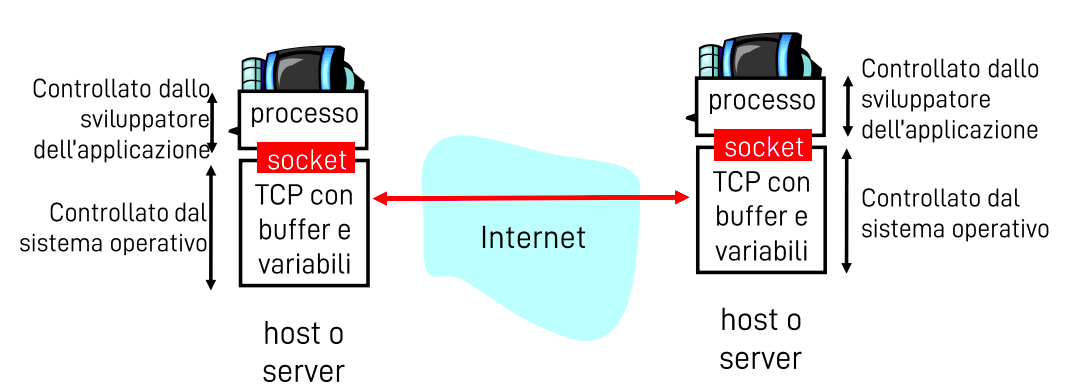
\includegraphics[width=\textwidth]{socket-tcp.png}
    \caption{Funzionamento \emph{socket TCP}}
\end{figure}\noindent
Al momento della creazione della \emph{server socket} viene specificato il
\emph{numero della porta} sulla quale il server si metterà in ascolto, mentre
nella creazione della \emph{client socket} vengono specificati
l'\emph{indirizzo IP} e il \emph{numero di porta} del processo server.

Inoltre, quando il client crea la \emph{socket} viene stabilita una connessione
\emph{TCP} con il server, il quale, risponde creando una nuova \emph{socket} per
comunicare con quel client. Questo comportamento consente al server di comunicare
con più client contemporaneamente distinguendoli in base alla
\emph{porta sorgente}\footnote{Nel corso della trattazione questo verrà reso
più chiaro}.

\begin{figure}[ht]
    \centering
    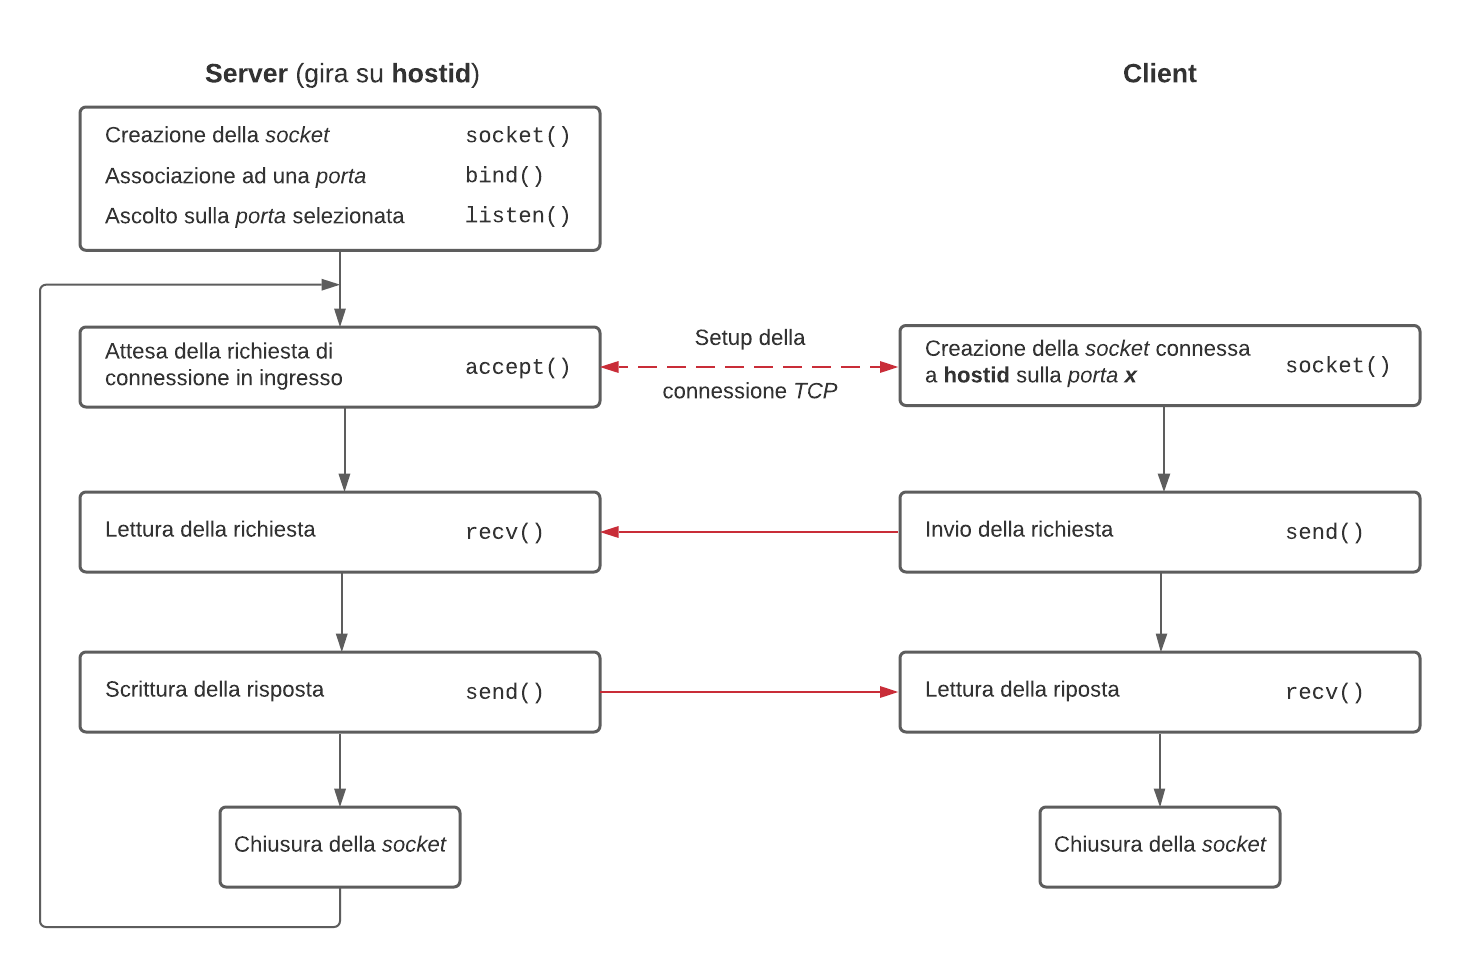
\includegraphics[scale=0.3]{socket-tcp-funzionamento.png}
    \caption{Comunicazione tra \emph{socket TCP}}
\end{figure}

\paragraph{Socket UDP}
Le \emph{socket UDP} comunicano utilizzando il protocollo \emph{UDP} e,
diversamente da quanto avviene nelle \emph{socket TCP}, il client non si connette
con il server, ma include in ogni pacchetto l'\emph{indirizzo IP} e il
\emph{numero di porta} del processo server. Di conseguenza, il server, per
distinguere i client, deve estrarre da ogni pacchetto
l'\emph{indirizzo IP} e il \emph{numero di porta} del mittente.

\section{Protocolli del livello Applicativo}
Prima di passare alla discussione sui protocolli più importanti del
\emph{livello Applicativo} è meglio chiarire la terminologia.

Una pagina web è costituita da \emph{oggetti}; un \emph{oggetto} può essere un
file \emph{\gls{glos:HTML}}, un'immagine, un file audio, \dots; una pagina web è
costituita da un file base scritto in \emph{HTML}, che solitamente include altri
oggetti referenziati; ogni oggetto è referenziato da un \emph{\gls{glos:URL}}.
\begin{definition}[URL]
    Un URL è una sequenza di caratteri che identifica univocamente una
    risorsa nella rete. La struttura di un URL è la seguente:

    \centering\scalebox{0.77}{
    {\tt
    protocollo://[username[:password]@]host[:porta][</percorso>][?querystring][\#fragment]
    }}
\end{definition}

\subsection{Protocollo HTTP}
L'\emph{\gls{prot:HTTP}} è un protocollo basato sul modello \emph{client-server}:
il ruolo di \emph{client} è ricoperto dai browser che richiedono, e ricevono,
oggetti dai \emph{server web}. La comunicazione tra \emph{client} e \emph{server}
si realizza tramite lo scambio di messaggi, che vengono scambiati sfruttando
\emph{socket TCP}. In particolare, il \emph{client} crea una connessione
\emph{TCP} sulla porta 80 del \emph{server}, il quale risponde accettando la
connessione. Questa connessione viene poi chiusa al termine dello scambio di
messaggi.

\paragraph{Connessioni persistenti e non}
Le \emph{connessioni HTTP}, ovvero le \emph{connessioni TCP} create dal
protocollo \emph{HTTP}, possono essere di due tipi:
\begin{itemize}
    \item \emph{Persistenti}: prima che la connessione venga chiusa possono
    essere trasmessi più oggetti;
    \item \emph{Non persistenti}: prima che la connessione venga chiusa viene
    trasmesso un solo oggetto;
\end{itemize}
\begin{definition}[\gls{glos:RTT}]
    È definito RTT il tempo di propagazione di andata e ritorno tra due host.
\end{definition}
\begin{note}
    Con \emph{tempo di propagazione} si intende, ad esempio, il tempo impiegato
    da un piccolo pacchetto per andare dal \emph{client} al \emph{server} e
    ritornare al \emph{client}.
\end{note}
Le \emph{connessioni non persistenti} hanno un \emph{RTT} doppio perché per ogni
oggetto va riaperta una nuova \emph{connessione TCP}. Questa caratteristica
porta anche il server a dover far fronte ad un maggiore overhead del sistema
operativo che deve gestire l'apertura di tutte quelle connessioni \emph{TCP}.
Inoltre, spesso accade che i browser aprano più connessioni in parallelo per il
trasferimento degli oggetti referenziati.

Con \emph{connessioni persistenti} tutte questi problemi non si presentano, ma
se il \emph{server} comunicasse con molti \emph{client} potrebbe terminare tutte le
porte disponibili e quindi potrebbe non poter più aprire nuove connessioni.

L'\emph{HTTP/1.0} utilizzava \emph{connessioni non persistenti}, mentre
dalla versione \emph{1.1} utilizza \emph{connessioni persistenti}.

\paragraph{Struttura dei messaggi}
Il protocollo \emph{HTTP} prevede due tipi di messaggi:
\begin{itemize}
    \item \emph{Richieste HTTP}: sono inviate dal \emph{client};
    \item \emph{Risposte HTTP}: sono inviate dal \emph{server} in risposta ad
    una richiesta;
\end{itemize}
I messaggi di \emph{richiesta} hanno la seguente struttura:
\begin{figure}[h!]
    \centering
    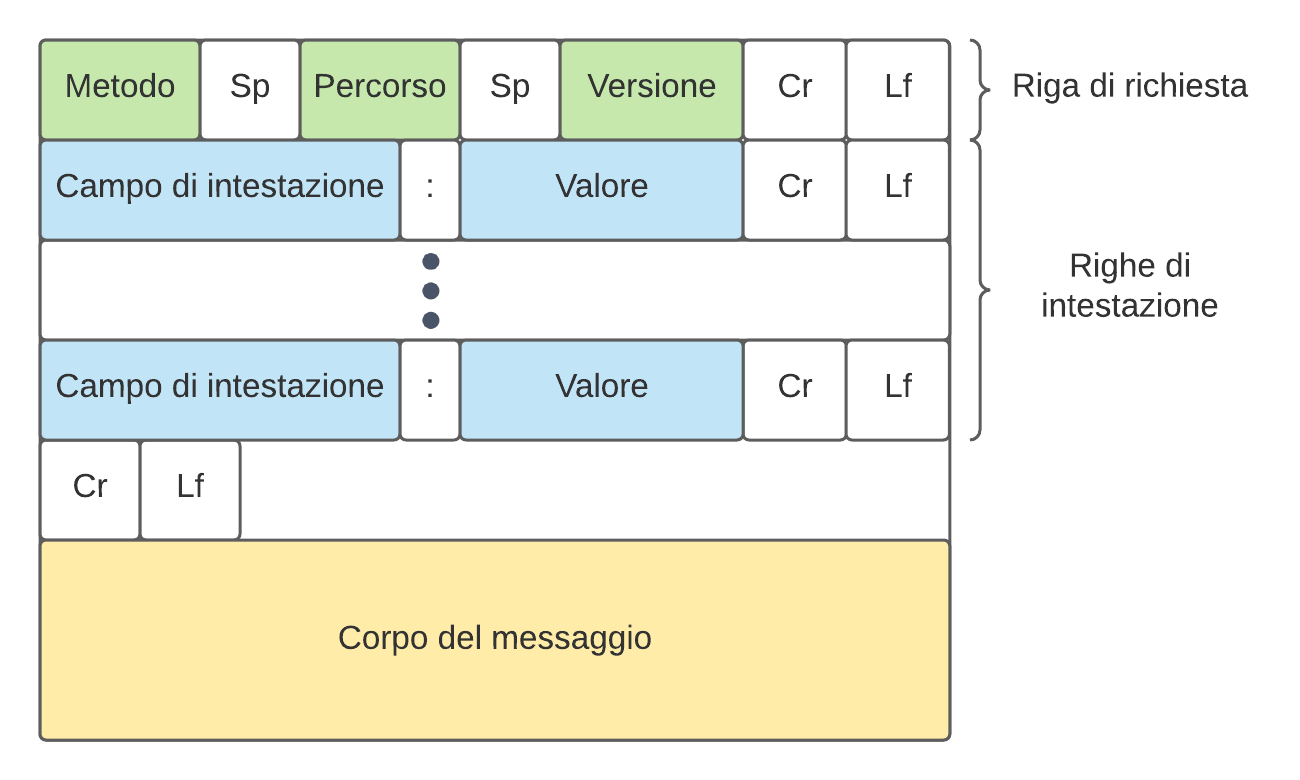
\includegraphics[width=\textwidth]{richiesta-http-struttura.png}
    \caption{Struttura messaggio di \emph{richiesta HTTP}}
\end{figure}

\noindent Il campo \emph{metodo} può essere uno dei seguenti:
\begin{itemize}
    \item \emph{GET}: richiede un file al \emph{server} scrivendo il percorso, ed
    eventuali altri dati, in chiaro nell’\emph{URL};
    \item \emph{POST}: invia informazioni all’\emph{URL} specificato scrivendo
    i dati nel corpo del \emph{messaggio HTTP};
    \item \emph{PUT}: carica un file sul \emph{server};
    \item \emph{HEAD}: richiede solo l’header della risposta senza la risorsa;
    \item \emph{OPTIONS}: richiede l’elenco dei metodi permessi dal \emph{server};
    \item \emph{DELETE}: cancella una risorsa sul \emph{server};
    \item \emph{TRACE}: traccia una richiesta visualizzando come viene trattata
    dal \emph{server};    
\end{itemize}
La \emph{versione} invece può essere uno tra: \emph{HTTP/1.0}, \emph{HTTP/1.1} e
\emph{HTTP/2.0}. Tra le \emph{righe d'intestazione} deve obbligatoriamente
essere presente il campo \emph{host} nel quale è indicato il nome dell'\emph{host}
da raggiungere.

I messaggi di \emph{risposta} hanno una struttura pressoché uguale:
\begin{figure}[ht]
    \centering
    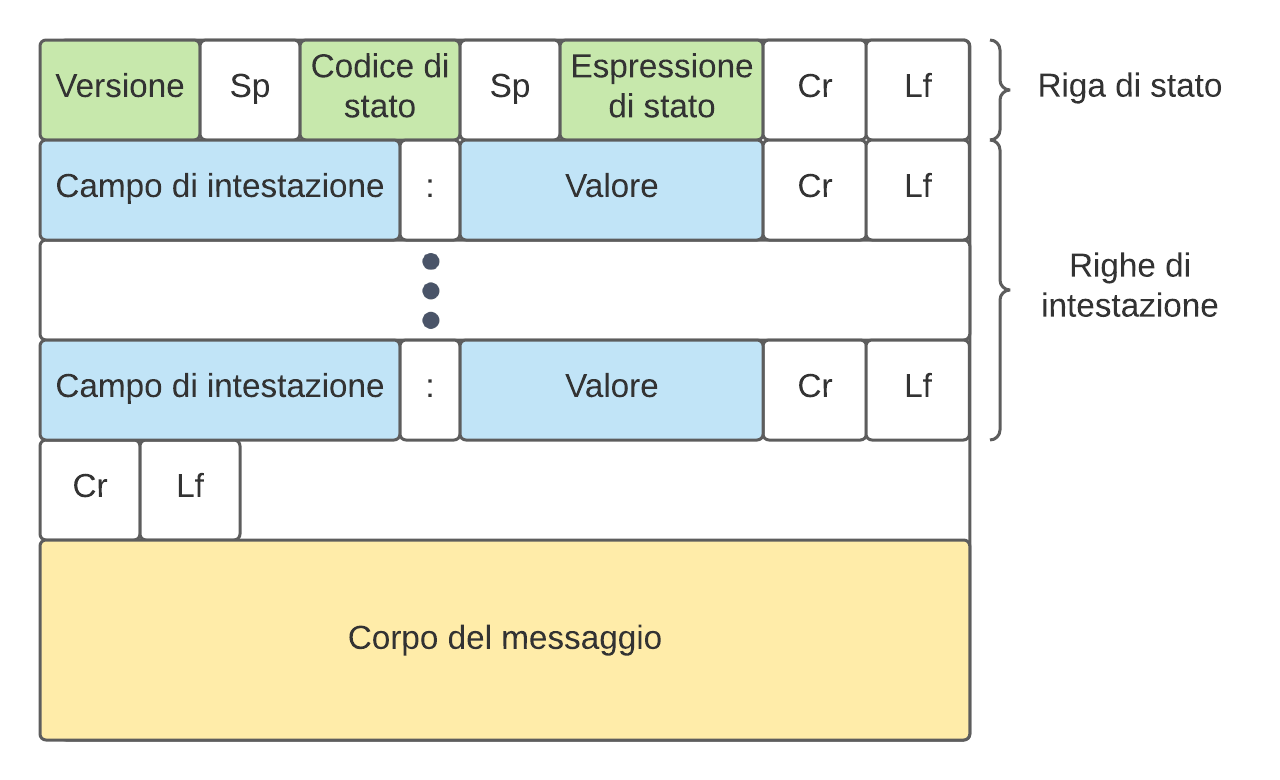
\includegraphics[width=\textwidth]{risposta-http-struttura.png}
    \caption{Struttura messaggio di \emph{risposta HTTP}}
\end{figure}

\noindent Il \emph{codice di stato} è un numero di tre cifre che identifica il
tipo di \emph{risposta} ed è definito secondo il seguente formato:
\begin{itemize}
    \item \emph{1XX}: richiesta ricevuta, risposta in arrivo;
    \item \emph{2XX}: richiesta ricevuta e soddisfatta;
    \item \emph{3XX}: ridirezione necessaria;
    \item \emph{4XX}: errore del client;
    \item \emph{5XX}: errore del server;
\end{itemize}
L'\emph{espressione di stato} è invece una descrizione del \emph{codice di stato}.

\paragraph{HTTP/2.0}
Il protocollo \emph{HTTP/2.0} è un'evoluzione dell'\emph{HTTP/1.1} ed è progettato
per ridurre la latenza percepita dall'utente e l'utilizzo delle risorse di rete
e dei server.

In particolare, l'\emph{HTTP/2.0} tenta di utilizzare un'unica connessione
tra client e server per richiedere tutte le risorse. È basato su
\emph{\gls{prot:SPDY}}, un protocollo del \emph{livello Applicativo} per il
trasporto di contenuti sul web con latenza minima. Per fare ciò, combina tre fattori:
\begin{itemize}
    \item \emph{Multiplexing di flussi}: su una singola \emph{connessione TCP}
    possono transitare un numero illimitato di flussi di dati;
    \item \emph{Priorità delle richieste}: il client può inviare un numero
    indefinito di richieste, specificando per ciascuna una priorità;
    \item \emph{Compressione dell'header HTTP}: l'header \emph{HTTP} viene
    compresso in modo da usare un minor numero di byte;
\end{itemize}
Il protocollo \emph{HTTP/2.0} introduce un livello intermedio tra il \emph{livello
Applicativo} e il \emph{Trasporto} (in realtà tra l'\emph{Applicativo} e il
\emph{Sessione}), chiamato \emph{binary framing}. Questo livello si occupa di
gestire le modalità di incapsulamento e trasferimento dei \emph{messaggi HTTP}.

\begin{figure}[h]
    \centering
    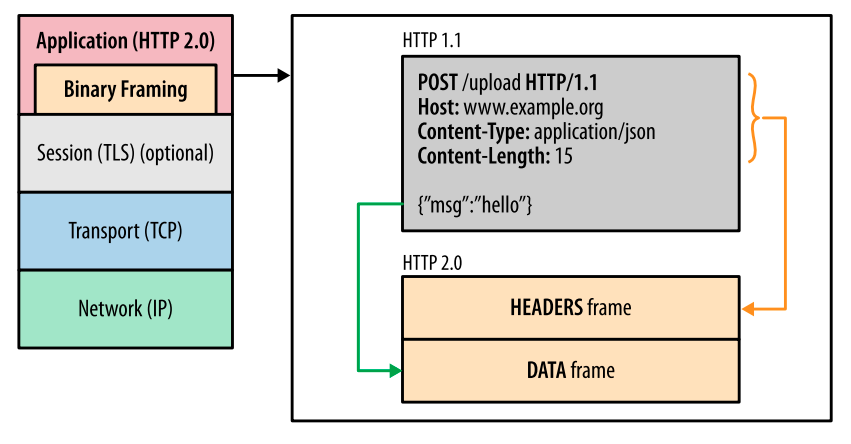
\includegraphics[width=0.7\textwidth]{binary-framing.png}
    \caption{Livello \emph{binary framing}}
\end{figure}\noindent
Il \emph{framing binario} lascia invariata la semantica dell'\emph{HTTP}, ma ne
modifica la codifica in fase di transito: ogni \emph{messaggio HTTP} è
suddiviso in \emph{frame} più piccoli codificati in binario.

\begin{note}
    Questa caratteristica dell'\emph{HTTP/2.0} lo rende incompatibile con le
    precedenti versioni, quindi server \emph{HTTP/1.x} e \emph{HTTP/2.0} non
    possono comunicare tra loro.
\end{note}\noindent
Ogni \emph{frame} è identificato da un valore univoco ed eventualmente anche da
un livello di priorità. Ogni messaggio trasmesso, che sia una richiesta o una
risposta, può essere suddiviso in uno o più \emph{frame} e ogni \emph{frame}
trasporta un tipo specifico di dati: \emph{header} o \emph{payload}.

\newpage
\begin{figure}[h]
    \centering
    \subfloat{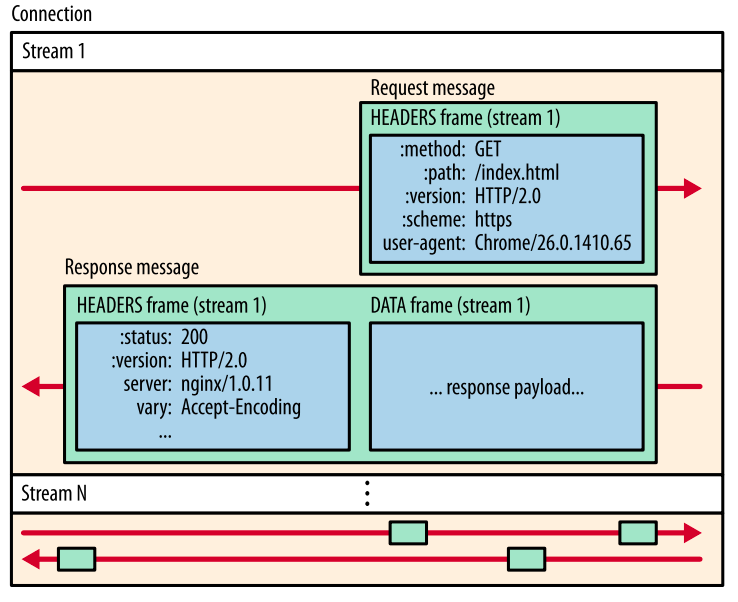
\includegraphics[scale=0.3, valign=c]{http2-stream.png}}
    \hfill
    \subfloat{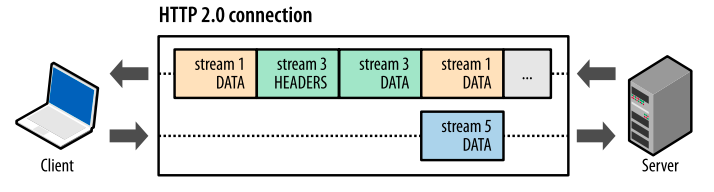
\includegraphics[scale=0.35, valign=c]{http2-frame.png}}
    \caption{Trasmissione dei \emph{frame} negli \emph{stream}}
\end{figure}

\bigskip\hspace{-0.5cm} Tutte le comunicazioni avvengono all'interno di un'unica
\emph{connessione TCP} che può trasportare un numero illimitato di \emph{stream}
bidirezionali di byte. Su ogni \emph{frame} è indicato l'identificativo unico
dello \emph{stream} sul quale sta viaggiando e questo consente di inviare i
\emph{frame} in modo indipendente, intervallandoli e ricomponendoli all'arrivo.

L'ordine di invio dei \emph{frame} dipende, qualora sia stata impostata, dalla
priorità indicata in senso crescente con un numero da 1 a 256. L'ordine di invio
dei \emph{frame} viene deciso dal server in base alle indicazioni fornitegli dal
client tramite un \emph{albero di priorità}.

\bigskip In \emph{HTTP/2.0} esiste quindi una sola \emph{connessione TCP
persistente}.

\begin{figure}[h!]
    \centering
    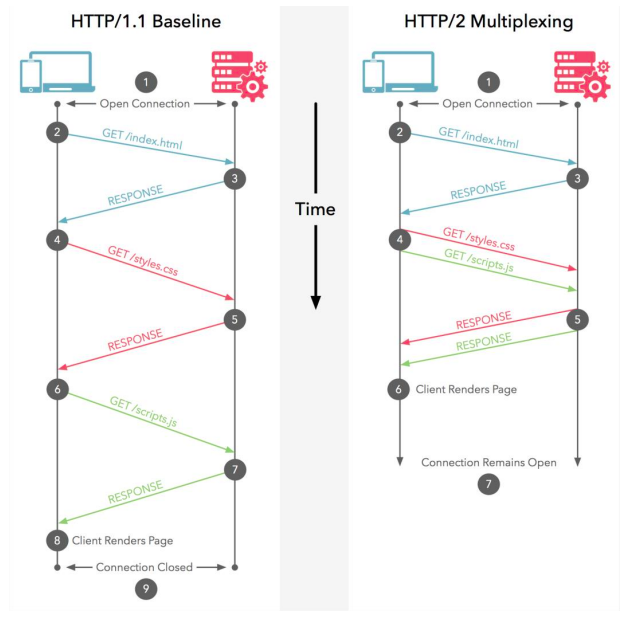
\includegraphics[width=0.7\textwidth]{http2-connessione.png}
    \caption{Connessione \emph{HTTP/1.1} VS \emph{HTTP/2}}
\end{figure}\noindent
Per tentare di ridurre ulteriormente la latenza, l'\emph{HTTP/2.0} introduce il
concetto di \emph{server push}. Quando il client fa una richiesta al server, questo
oltre alla risorsa richiesta invia anche altre risorse ad essa collegate. Queste
risorse inviate in più dal server sono dette \emph{server promise}.

\begin{figure}[h]
    \centering
    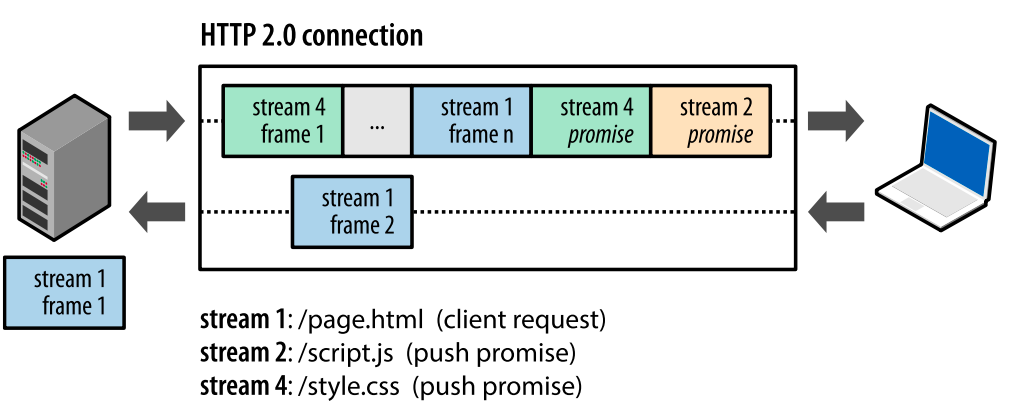
\includegraphics[width=0.7\textwidth]{http2-server-push.png}
    \caption{\emph{HTTP/2.0 server push}}
\end{figure}

\paragraph{Comunicazioni senza stato e i cookie}
Nell'\emph{HTTP} la comunicazione tra client e server è priva di stato, ciò
significa che il server non ha memoria delle precedenti richieste di un client.

Per simulare lo stato si usano i \emph{cookie}, ovvero file generati dal web
server e salvati sul client che contengono, tra le altre cose, informazioni sulle
preferenze di un client riguardo un sito web (e.g. carrello della
spesa nei siti di e-commerce).

In particolare, i \emph{cookie} sono file contenenti una stringa di testo, una
data di scadenza e un pattern per il riconoscimento dei domini di destinazione
che vengono inviati al web server ogni volta che il client accede ad una pagina
del sito.
La stringa di testo contenuta in un cookie è detta \emph{chiave di sessione} ed
è utilizzata per identificare in modo univoco un client e i relativi dati
che vengono salvati in un database accessibile al server web.

\begin{figure}[h]
    \centering
    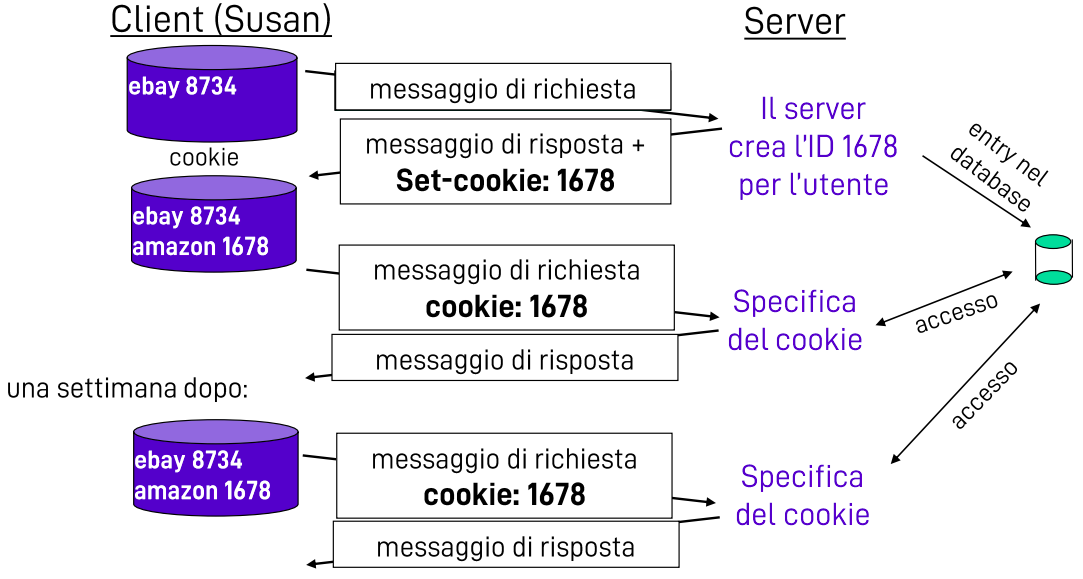
\includegraphics[width=\textwidth]{http-cookie.png}
    \caption{Utilizzo dei \emph{cookie}}
\end{figure}\noindent
La prima volta che un client accede ad una pagina web, il server crea una
\emph{chiave di sessione} e ne specifica il valore nel campo \emph{Set-cookie}
dell'\emph{header HTTP} del messaggio di risposta. Il browser del client salva
quel valore e nelle successive richieste lo va ad inserire nell'\emph{header}
nel campo \emph{Cookie}.

\paragraph{Server proxy}
Il \emph{proxy} è un server intermedio che si pone tra client e server.
Quando un client richiede una risorsa al server, la richiesta viene prima
intercettata dal \emph{proxy} che verifica la presenza della risorsa nella propria
cache interna. Se nel \emph{proxy} la risorsa richiesta non è presente o non è
aggiornata, la richiesta viene inoltrata dal \emph{proxy} al server di destinazione.

Quindi, il \emph{proxy} riceve la risposta dal server e prima di inviarla al
client, provvede a salvarla al suo interno, così da poterla riutilizzare per future
richiese senza dover ricontattare il server.

Tuttavia, nel caso di risorse dinamiche è importante che queste siano aggiornate,
quindi quando il \emph{proxy} riceve una richiesta, invia un \emph{messaggio HTTP}
di tipo \emph{HEAD} al web server e confronta la data di ultima modifica della
pagina salvata con quella della pagina sul web server. Se la pagina salvata è
scaduta, il \emph{proxy} la aggiorna e risponde alla richiesta del client
con la versione aggiornata. In alternativa ad una richiesta \emph{HEAD} seguita
da una \emph{GET}, il \emph{proxy} può utilizzare una \emph{GET condizionale} che
richiede la risorsa solo se la data di ultima modifica è successiva a quella
indicata nell'\emph{header} nel campo \emph{If-modified-since}.

\begin{figure}[h]
    \centering
    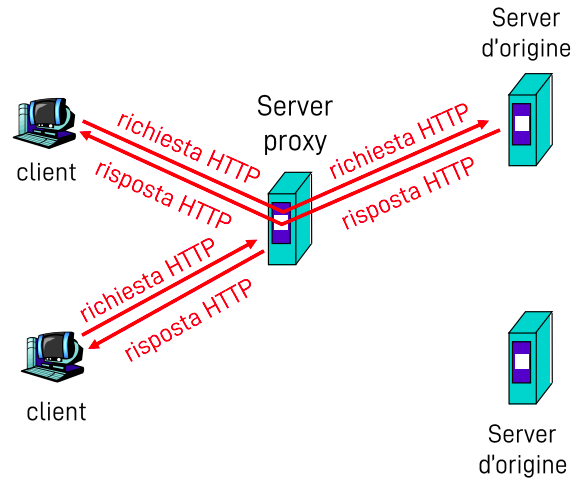
\includegraphics[width=0.7\textwidth]{http-proxy.png}
    \caption{Server \emph{proxy}}
\end{figure}

\subsection{Protocollo FTP}
L'\emph{\gls{prot:FTP}} è un protocollo \emph{client-server} per il trasferimento
di file tra client e server. Vengono usate due connessioni \emph{TCP} sulle
porte 21 e 22 del server. La prima è dedicata allo scambio dei comandi, mentre la
secondo, viene aperta all'occorrenza e viene mantenuta attiva soltanto per il
tempo necessario, ed è usata per il trasferimento dei file.

\begin{figure}[ht]
    \centering
    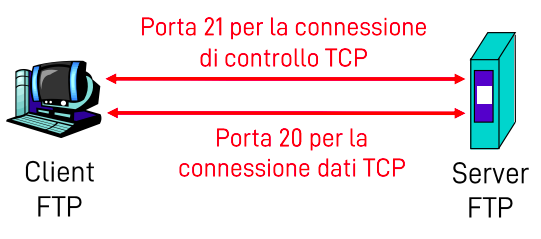
\includegraphics[width=0.7\textwidth]{ftp.png}
    \caption{Connessioni aperte dall'\emph{FTP}}
\end{figure}

\newpage
\subsection{Protocolli per la posta elettronica}
Nello scambio di messaggi di posta elettronica gli attori principali sono tre:
\begin{itemize}
    \item \emph{Agente utente}: permette la composizione e la lettura delle email;
    \item \emph{Server di posta}: contiene i messaggi da recapitare all'utente e la
    coda di messaggi da trasmettere;
    \item \emph{Protocollo di trasferimento}: gestisce il trasporto di email tra
    utente e server e tra server;
\end{itemize}

\paragraph{Protocollo SMTP}
È utilizzato per mettere in comunicazione i \emph{server di posta} e, in particolare,
trasmette i messaggi direttamente tra il server mittente e il server destinatario.
Il trasferimento è articolato in tre fasi: \emph{handshake}, \emph{trasferimento}
e \emph{chiusura}.

L'interazione tra i server avviene mediante messaggi in formato ASCII a 7 bit; ad
ogni comando corrisponde un messaggio di risposta formato da un codice di stato e
un'espressione. Inoltre, l'\emph{\gls{prot:SMTP}} trasmette più oggetti all'interno
di uno stesso messaggio e utilizza \emph{connessioni persistenti}.

\begin{figure}[h!]
    \centering
    \begin{lstlisting}[basicstyle=\scriptsize]
        S: 220 hamburger.edu
        C: HELO crepes.fr
        S: 250 Hello crepes.fr, pleased to meet you
        C: MAIL FROM: <alice@crepes.fr>
        S: 250 alice@crepes.fr... Sender ok
        C: RCPT TO: <rob@hamburger.edu>
        S: 250 rob@hamburger.edu ... Recipient ok
        C: DATA
        S: 354 Enter mail, end with "." on a line by itself
        C: From: alice@crepes.fr
        C: To: bob@hamburger.edu
        C: Subject: Important question.
        C: 
        C: Do you like ketchup?
        C: .
        S: 250 Message accepted for delivery
        C: QUIT
        S: 221 hamburger.edu closing connection
    \end{lstlisting}
    \caption{Esempio di interazione tra \emph{server SMTP}}
\end{figure}\noindent
È possibile trasmettere anche oggetti multimediali utilizzando l'estensione
\emph{MIME} e codificando i dati da trasmettere usando la codifica \emph{base64}
che rappresenta 6 bit usandone 8.

Per utilizzare l'estensione \emph{MIME} è sufficiente aggiungere nell'intestazione
del messaggio le seguenti tre righe:
\newpage
\begin{figure}[ht]
    \centering
    \begin{lstlisting}[basicstyle=\scriptsize]
        MIME-Version: 1.0
        Content-Transfer-Encoding: base64
        Content-Type: image/jpeg
    \end{lstlisting}
    \caption{Intestazione per messaggi multimediali}
\end{figure}\noindent
Ovviamente il \texttt{Content-type} dipende dal tipo di oggetto che si vuole
trasferire.

\paragraph{Protocolli POP3 e IMAP4}
\emph{\gls{prot:POP}} e \emph{\gls{prot:IMAP}} sono usati per il trasferimento
di messaggi tra \emph{server} e \emph{agenti utente}. Entrambi utilizzano
il protocollo \emph{\gls{prot:TCP}} per lo scambio di messaggi, ma a parte questo
sono basati su filosofie opposte.

Il protocollo \emph{POP3} prevede che l'utente si colleghi al server e scarichi
tutte le email disponibili. Una volta scaricate, le email vengono eliminate dal
server. D'altra parte, il protocollo \emph{IMAP4} consente all'utente di accedere
alle email mantenendole nel server e inoltre permette l'organizzazione dei
messaggi in cartelle. Per questo motivo, l'\emph{IMAP4} mantiene lo stato
dell'utente tra le varie sessioni, mentre il \emph{POP3} no.

\begin{figure}[h!]
    \centering
    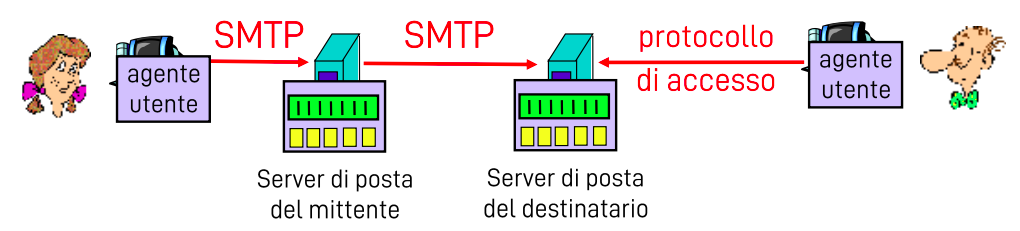
\includegraphics[width=\textwidth]{email.png}
    \caption{Scambio di email}
\end{figure}

\begin{note}
    Ci si potrebbe chiedere perché non si usi soltanto l'\emph{SMTP}.
    La risposta è che l'\emph{SMTP} può trasmettere un messaggio soltanto se
    il ricevente è online.
\end{note}

\paragraph{Protocollo TLS}
Il \emph{\gls{prot:TLS}} è un protocollo che consente di rendere sicura la
comunicazione tra due entità fornendo:
\begin{itemize}
    \item \emph{Autenticazione}: l'identità di mittente e destinatario viene
    verificata;
    \item \emph{Integrità dei dati}: viene garantito che il messaggio non verrà
    manipolato durante la trasmissione;
    \item \emph{Confidenzialità}: soltanto il legittimo destinatario sarà in
    grado di accedere al contenuto del messaggio;
\end{itemize}
Il funzionamento del \emph{TLS} può essere suddiviso in tre fasi:
\emph{negoziazione fra le parti dell'algoritmo da utilizzare}, \emph{scambio delle
chiavi e autenticazione}, \emph{cifratura simmetrica e autenticazione dei messaggi}.

È possibile combinare i tre protocolli per lo scambio di email con il
\emph{TLS} per rendere sicuro lo scambio di messaggi. Ovviamente, un \emph{host}
che non utilizza questa tecnologia non può comunicare con un altro \emph{host} che
la usa, quindi, vengono usati \emph{numeri di porta} diversi dalle versioni
\quotes{non sicure} di quei protocolli.

\bigskip\noindent
Esiste un'evoluzione del \emph{TLS} chiamata \emph{STARTTLS} che consente
di comunicare sulle porte originali dei protocolli. In particolare, il client
che intende assicurare la comunicazione, chiede al server l'instaurazione di una
connessione cifrata, la sessione inizia in chiaro e diventa cifrata prima che
vengano trasmessi dati sensibili.

\subsection{Protocollo DNS}
Ad ogni \emph{nome di dominio} è associato un \emph{indirizzo IP} (in realtà anche
più di uno); il protocollo \emph{\gls{prot:DNS}} consente di risolvere i \emph{nomi
di dominio}, ovvero di risalire all'\emph{indirizzo IP} associato a un \emph{nome}.
Oltre a ciò, altri servizi offerti dal \emph{DNS} sono:
\begin{itemize}
    \item \emph{Host aliasing}: è possibile associare degli alias ad un \emph{nome
    di dominio};
    \item \emph{Mail server aliasing}: come per l'\emph{host aliasing}, ma per i
    server mail;
    \item \emph{Load distribution}: il \emph{DNS} può essere usato per distribuire
    il carico delle richieste tra più server replicati, cioè con lo stesso nome.
    Ciò è possibile perché quando un \emph{server DNS} riceve una richiesta,
    restituisce, se possibile, più di un \emph{indirizzo IP}. L’ordine degli
    \emph{indirizzi IP} dei server replicati viene cambiato ad ogni richiesta in
    modo da evitare che le richieste arrivino sempre ad unico server, congestionandolo;
\end{itemize}

\paragraph{Struttura dei nomi di dominio}
Prima di procedere oltre è bene chiarire i termini usati per descrivere i
\emph{nomi di dominio}. Il nome \texttt{drive.google.com.}, ad esempio, si
struttura, a partire da destra, in:
\begin{itemize}
    \item \emph{Root}: è implicito in ogni nome ed è indicato con un punto
    \texttt{(.)};
    \item \emph{\gls{glos:TLD}}: è il \emph{dominio di primo livello} e può
    essere generico (e.g. \texttt{.com}, \texttt{.org}, \dots) o nazionale (e.g.
    \texttt{.it}, \texttt{.de}, \dots);
    \item \emph{\gls{glos:SLD}}: è il \emph{dominio di secondo livello}
    (\texttt{.google});
    \item \emph{Sottodominio}: è un sottodominio del \emph{SLD} e server ad
    indentificare uno specifico \emph{host} o gruppo di \emph{host} all'interno
    del dominio (\texttt{drive});
\end{itemize}

\paragraph{Implementazione del DNS}
Il \emph{DNS} è implementato come una gerarchia di database distribuiti.
Partendo dal vertice, la gerarchia di server DNS è organizzata in tre livelli:
\begin{itemize}
    \item \emph{Root server}: sono 13 in tutto il mondo e conoscono la posizione
    dei server che gestiscono i \emph{TLD};
    \item \emph{TLD server}: gestiscono i \emph{TLD} e conoscono la posizione degli
    \emph{authoritative server} (\emph{server di competenza}) che gestiscono i
    \emph{SLD} di una determinata zona;
    \item \emph{Authoritative server}: gestiscono i \emph{SLD} e sanno risolvere
    tutti i nomi di dominio della loro zona di competenza;
\end{itemize}
Esistono 13 \emph{root server} logici nel mondo, ma ognuno di essi è pesantemente
ridondato per evitare interruzioni di servizio o perdite di dati. Anche i
\emph{TLD} e gli \emph{authoritative server} sono ridondati per scongiurare
congestioni, sovraccarichi e gli altri problemi visti per i \emph{root server}.

Oltre ai server della gerarchia, ogni \emph{\gls{glos:ISP}} ha un proprio
\emph{server DNS locale} detto \emph{default name server} che riceve le richieste
fatte dagli \emph{host} della rete, le inoltra ai server della gerarchia e infine
restituisce all'\emph{host} interessato il risultato dell'interrogazione.

Gli \emph{host} interrogano i \emph{server DNS} sfruttando le funzioni fornite da
un \emph{resolver}. Si tratta di un’applicazione client, generalmente integrata
nel sistema operativo, che permette di realizzare la risoluzione dei \emph{nomi di
dominio}.

\begin{note}
    Ci si potrebbe chiedere perché non venga usato un unico server centralizzato.
    Il motivo è che una soluzione del genere comporterebbe enormi problematiche,
    quali:
    \begin{itemize}
        \item \emph{\gls{glos:SPOF}}: il server diventerebbe un \emph{SPOF} col
        risultato che un suo guasto renderebbe il servizio inutilizzabile in
        tutta la rete;
        \item \emph{Volume di traffico}: dovendo gestire le richieste di tutta la
        rete il server sarebbe costantemente congestionato;
        \item \emph{Distanza}: il server sarebbe stato distante dalla maggior parte
        degli utenti e per alcuni addirittura irraggiungibile per via del limite di
        \emph{hop};
        \item \emph{Manutenzione permanente}: il server dovrebbe essere costantemente
        aggiornato per aggiungere e modificare i dati esistenti rendendolo
        inutilizzabile per la maggior parte del tempo;
        \item \emph{Non scalabilità}: il server avrebbe avuto molte difficoltà ad
        adattarsi ai mutamenti del volume di traffico della rete;
    \end{itemize}
\end{note}

\begin{figure}[h]
    \centering
    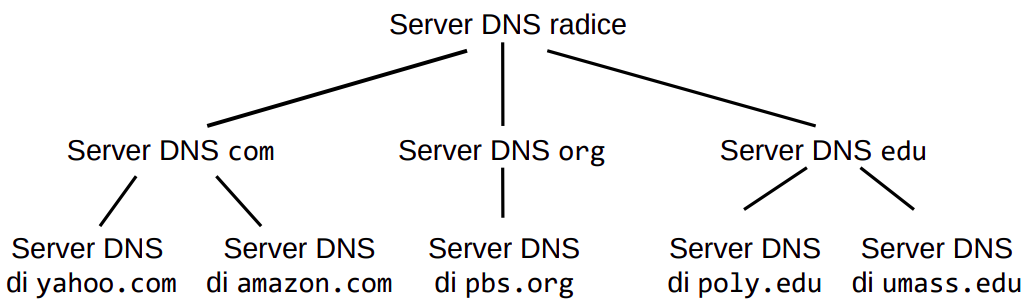
\includegraphics[width=\textwidth]{gerarchia-dns.png}
    \caption{Gerarchia dei \emph{server DNS}}
\end{figure}

\paragraph{Interrogare i server}
Quando un \emph{host} intende risolvere un \emph{nome di dominio} contatta il
proprio \emph{default name server}. Se questo ha già la risposta all'interrogazione
ricevuta, la restituisce direttamente all'\emph{host}, altrimenti interroga la
gerarchia. Per fare questo esistono due modalità: \emph{iterativa} e \emph{ricorsiva}.

Nella modalità \emph{iterativa} il \emph{server DNS locale} procede ad interrogare
ogni livello della gerarchia. Partendo dal \emph{root server}, richiede l'indirizzo
del \emph{TLD server} associato al \emph{TLD} da risolvere, quindi interroga il
\emph{server di competenza} per il \emph{nome} completo.

D'altra parte, nella modalità \emph{ricorsiva}, il \emph{server DNS locale}
interroga il \emph{root server}, questo quindi interroga il \emph{TLD server} che
a sua volta interroga l'\emph{authoritative server}. Una volta trovata la risposta
questa risale la gerarchia fino a tornare al \emph{default name server}.

Solitamente i \emph{server DNS} non rispondono a richieste fatte in modalità
\emph{ricorsiva} perché sono causa di congestione.

\newpage
\begin{figure}[ht]
    \centering
    \subfloat[Query \emph{iterativa}]{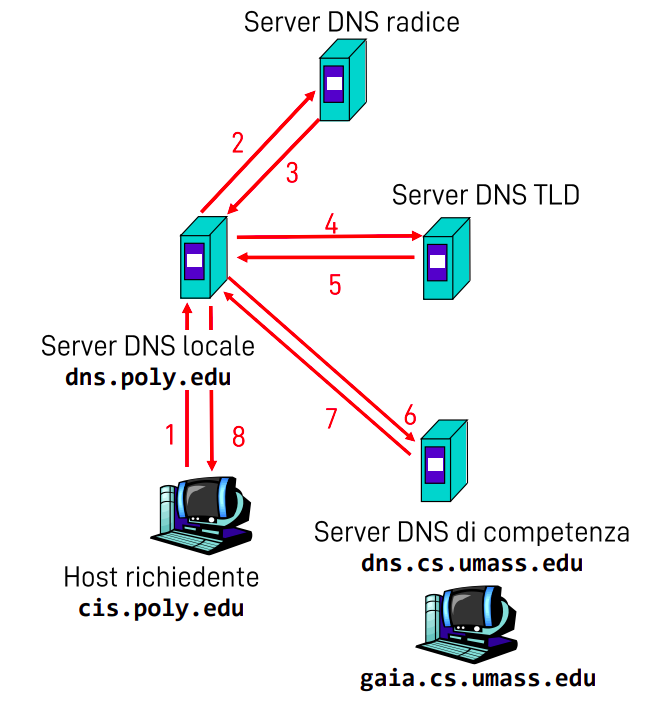
\includegraphics[width=0.5\textwidth]{query-iterativa.png}}
    \hfill
    \subfloat[Query \emph{ricorsiva}]{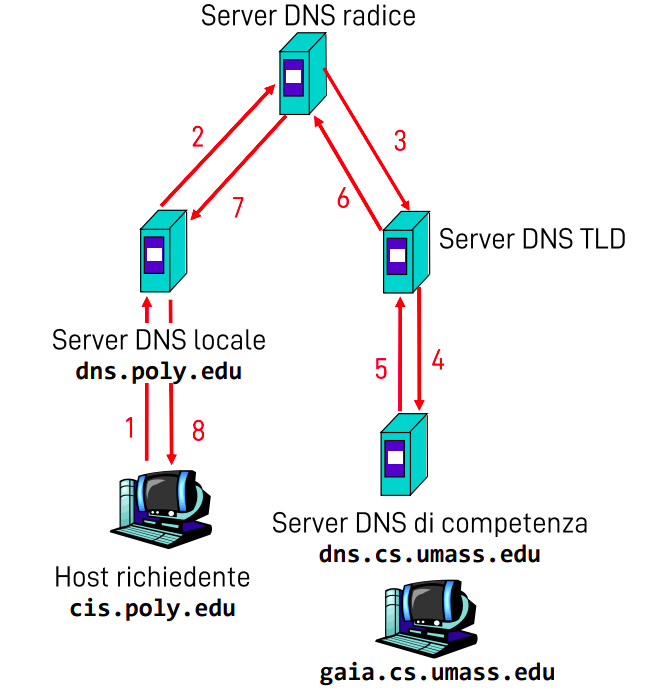
\includegraphics[width=0.5\textwidth]{query-ricorsiva.png}}
    \caption{Query \emph{iterativa} VS query \emph{ricorsiva}}
\end{figure}

\paragraph{DNS caching}
Quando un \emph{server DNS} impara la mappatura di una di un \emph{nome di dominio},
la salva in una cache. Queste informazioni vengono invalidate dopo un certo periodo
di tempo in modo da costringere l'aggiornamento dei dati.

Solitamente, per evitare di contattare i \emph{root server}, i \emph{server DNS
locali} salvano gli indirizzi dei \emph{TLD server}.

\paragraph{Resource record}
I \emph{server DNS} memorizzano le informazioni in \emph{\gls{glos:RR}} con questo
formato:
\[\texttt{(name, value, type, ttl)}\]
I valori più comuni per il campo \texttt{type} sono:
\begin{itemize}
    \item \texttt{A}: associa il \emph{nome di dominio} a un indirizzo \emph{IPv4}
    (\texttt{name}: \emph{nome di dominio}, \texttt{value}: \emph{indirizzo IPv4});
    \item \texttt{AAAA}: come il precedente, ma associa un indirizzo \emph{IPv6};
    \item \texttt{CNAME}: associa un \emph{alias} al \emph{nome canonico}
    (\texttt{name}: \emph{alias}, \texttt{value}: \emph{nome canonico});
    \item \texttt{MX}: associa a un \emph{nome di dominio} il proprio \emph{mail
    server} (\texttt{name}: \emph{nome di dominio}, \texttt{value}: nome del
    \emph{mail server});
    \item \texttt{NS}: associa al \emph{nome di dominio} il nome del relativo
    \emph{server di competenza} (\texttt{name}: \emph{dominio}, \texttt{value}:
    nome del \emph{server di competenza});
\end{itemize}

\paragraph{Messaggi DNS}
Il protocollo \emph{DNS} prevede due tipi di messaggi: \emph{domande} e
\emph{risposte}. Entrambi usano lo stesso formato.

\newpage
\begin{figure}[ht]
    \centering
    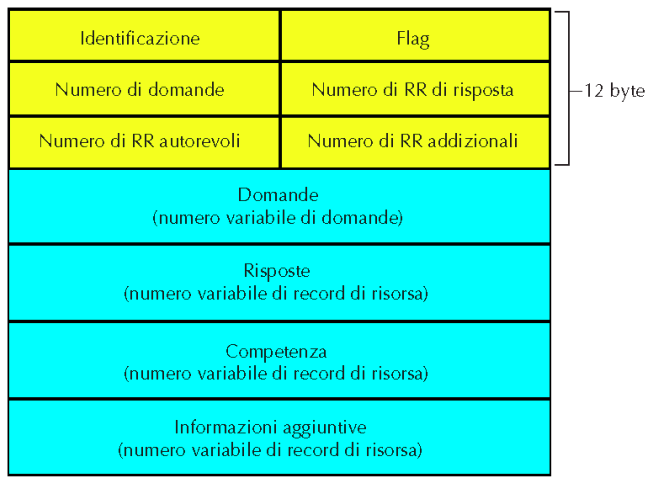
\includegraphics[width=0.7\textwidth]{messaggio-dns.png}
    \caption{Struttura di un messaggio \emph{DNS}}
\end{figure}\noindent
I campi descrivono:
\begin{itemize}
    \item \emph{Identificazione}: un valore di 16 bit che identifica in modo
    univoco una domanda e la relativa risposta;
    \item \emph{Flag}: i flag sono quattro:
    \begin{itemize}
        \item \emph{Domanda o risposta};
        \item \emph{Richiesta di ricorsione};
        \item \emph{Ricorsione disponibile};
        \item \emph{Risposta di competenza};
    \end{itemize}
    \item \emph{Domande}: campi per il \emph{nome} richiesto e il tipo di domanda;
    \item \emph{Risposte}: \emph{RR} di risposta alla domanda;
    \item \emph{Competenza}: \emph{RR} dedicati per i \emph{server di competenza};
    \item \emph{Informazioni aggiuntive}: informazioni extra che possono essere
    usate;
\end{itemize}

\paragraph{Inserire record nel database}
Quando si registra un \emph{nome di dominio} presso un \emph{registrar}, ovvero
una società che garantisce l'unicità del \emph{nome}, questa provvede ad inserire
nel database del \emph{server DNS} due \emph{RR}. Nel primo viene associato il
\emph{nome di dominio} al relativo \emph{server di competenza}, mentre nel
secondo associa il nome del \emph{server di competenza} al suo \emph{indirizzo IP}.
\chapter{Livello Trasporto}
I protocolli del \emph{livello Trasporto} forniscono strumenti per la
comunicazione logica tra processi di \emph{host} differenti e vengono eseguiti dai
sistemi terminali, cioè dal mittente per quello che riguarda l'invio dei dati e
dal destinatario per la ricezione.

\section{Caratteristiche dei servizi offerti}
Tipicamente, al momento dell'invio, i messaggi vengono suddivisi in \emph{segmenti}
e questi sono poi riassemblati al momento della ricezione.

I protocolli che appartengono a questo livello si appoggiano ai servizi
offerti dal \emph{livello Rete} che si occupa di gestire la comunicazione logica
tra \emph{host}. Quindi, il \emph{livello Trasporto} è di fatto un potenziamento del
\emph{livello Rete}.

\bigskip\noindent
I protocolli di \emph{trasporto} principali sono l'\emph{\gls{prot:UDP}} e il
\emph{\gls{prot:TCP}}. Questi due servizi si differenziano per la filosofia
con la quale si approcciano al trasporto dei dati: \emph{best effort} per
l'\emph{UDP} e \emph{affidabile} per il \emph{TCP}. Il \emph{TCP}, infatti, è
un \emph{protocollo connesso}, che garantisce l'arrivo di tutti i \emph{segmenti}
trasmessi permettendo al destinatario di ordinarli e occupandosi anche di gestire
il controllo della congestione e del flusso. D'altra parte, l'\emph{UDP} non
fa nulla di tutto ciò, ma trasmette i \emph{segmenti} cercando di ridurre al
minimo l'overhead; scelta che ovviamente non permette di assicurare l'arrivo
di tutti i dati.

\paragraph{Controllo di congestione e di flusso}
\emph{Controllo della congestione} e \emph{controllo del flusso} sono due
concetti molto diversi che è bene chiarire subito:
\begin{definition}[Controllo della congestione]
    Il controllo della congestione permette di evitare che il mittente
    trasmetta più dati di quelli che la rete può gestire.    
\end{definition}
\begin{definition}[Controllo del flusso]
    Il controllo del flusso permette di evitare che il mittente
    trasmetta più dati di quelli che il destinatario può gestire.
\end{definition}

\subsection{Multiplexing e demultiplexing}
\emph{Multiplexing} e \emph{demultiplexing} sono due operazioni realizzate
rispettivamente dal mittente e dal destinatario.

\noindent
Il \emph{multiplexing} consiste nell'aggiunta ai dati trasmessi dalle
\emph{socket} di un header con le \emph{\gls{glos:PCI}} del \emph{livello
Trasporto}. Le informazioni aggiunte consentono di identificare la \emph{socket
sorgente} e di \emph{destinazione}.
In fase di \emph{demultiplexing} invece, quelle stesse \emph{PCI} vengono usate
per consegnare i \emph{segmenti} ricevuti alla \emph{socket} corretta.

\paragraph{Funzionamento del demultiplexing}
L'\emph{host} riceve i \emph{pacchetti IP} che nel proprio header trasportano
gli \emph{indirizzo IP} sorgente e di destinazione. Ogni \emph{pacchetto IP} ha
come \emph{payload} un \emph{segmento} del \emph{livello Trasporto} nel cui header
sono indicati i \emph{numero di porta} sorgente e di destinazione.
L'\emph{host} utilizza quindi la coppia \emph{indirizzo IP-numero di porta} per
identificare la \emph{socket} alla quale consegnare il \emph{segmento}.
\begin{figure}[h!]
    \centering
    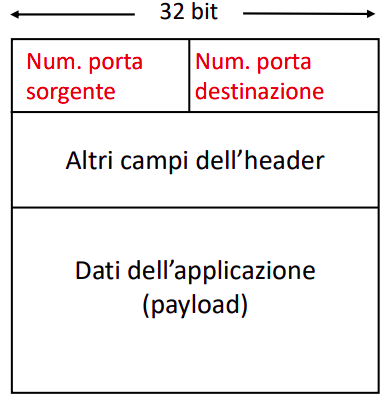
\includegraphics[width=0.4\textwidth]{segmento-livello-trasporto.png}
    \caption{Struttura di un \emph{segmento TCP/UDP}}
\end{figure}

\paragraph{Demultiplexing senza connessione}
Nel caso del protocollo \emph{UDP}, che è un protocollo non connesso, quando
l'\emph{host} riceve un \emph{segmento}, legge i parametri della \emph{socket} di
destinazione (\emph{indirizzo IP-numero di porta} di destinazione) e consegna
il \emph{segmento} a quella \emph{socket}. \emph{Segmenti} proveniente da
processi diversi, ma con gli stessi parametri di destinazione vengono anch'essi
destinati alla medesima.

\paragraph{Demultiplexing con connessione}
Il \emph{TCP}, invece, per identificare una \emph{socket}, usa anche i parametri
di sorgente, quindi l'\emph{host} ricevente utilizza tutti e quattro i parametri per
inviare il \emph{segmento} alla \emph{socket} appropriata. Questo è conseguenza
del fatto che un server può supportare più \emph{socket TPC} contemporaneamente.

\begin{note}
    I server \emph{HTTP} creano \emph{socket} differenti per ogni connessione con
    i client. E, addirittura, con versioni \emph{non-persistenti} dell'\emph{HTTP},
    si ha una \emph{socket} differente per ogni richiesta.
\end{note}

\subsection{Numeri di porta}
Quindi, la destinazione finale di un \emph{segmento} non è un \emph{host}, ma un processo
in esecuzione su un \emph{host}. L'interfaccia tra il \emph{livello Applicativo} e il
\emph{Trasporto} è costituita dal già citato \emph{numero di porta}: un valore
numerico a 16 bit che identifica univocamente un processo all'interno di un
\emph{host}.

I \emph{numeri di porta} per i servizi standardizzati sono noti e sono quindi detti
\emph{well-known}. Si tratta di valori compresi tra $0$ a $1023$ (incluso) che
identificano un processo che fornisce un servizio standardizzato (e.g porta 80
per l'\emph{HTTP}, porta 25 per l'\emph{SMTP}, \dots).

\noindent
I servizi non standard e le connessioni in ingresso a un client utilizzano invece
\emph{numeri di porta} con valori fino a $65535$ ($2^{16}-1$) che sono decisi in
modo automatico dal sistema operativo al momento della creazione di una
\emph{socket} o di instaurazione di una connessione.

\begin{note}
    Le \emph{porte well-known} sono anche dette \emph{statiche}, mentre quelle
    assegnate dal sistema operativo sono dette \emph{effimere}.
\end{note}\noindent
Una cosa importante da tenere a mente è che il \emph{numero di porta} sorgente e
di destinazione non sono quasi mai uguali.
Questo perché i server restano in ascolto su una porta nota ai client, quindi
quando un client contatta, o si connette con il server, lo fa su quella
\emph{porta}. Tuttavia, poiché più processi in esecuzione sullo stesso client
potrebbero contattare lo stesso server, è necessario che ogni processo del
client sia associato ad un \emph{numero di porta} diverso da quello degli altri.
Di conseguenza, non è possibile usare sempre lo stesso \emph{numero di porta}
scelto dal server. In relazione a ciò, è bene chiarire il concetto di
\emph{flusso di dati}:
\begin{definition}[Flusso di dati]
    Un flusso è un gruppo di dati che appartengono alla stessa comunicazione
    logica.
\end{definition}
\begin{note}
    Un'applicazione può aprire molteplici \emph{connessioni} e veicolare
    molti \emph{flussi}.
\end{note}

\section{Protocollo UDP}
Come già accennato, il protocollo \emph{UDP} è orientato alla \quotes{consegna
con minimo sforzo} (\emph{best effort}), col risultato che i \emph{segmenti UDP}
potrebbero non giungere mai a destinazione o arrivare in un ordine diverso da
quello di invio. È anche un protocollo non connesso quindi ogni \emph{segmento}
è gestito in modo indipendente dagli altri.

Se da una parte tutte queste caratteristiche rendono l'\emph{UDP} un protocollo
poco affidabile, lo rendono anche molto meno oneroso in termini di overhead e
ritardi amministrativi: gli header sono più corti, non esiste un ritardo
provocato dall'instaurazione di una connessione, non è necessario mantenere uno
stato della comunicazione e, non facendo controlli di congestione, può inviare
raffiche di dati.

\begin{figure}[h!]
    \centering
    \hspace{-2cm}
    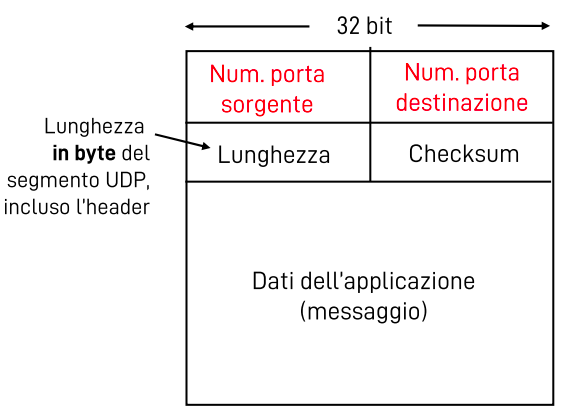
\includegraphics[width=0.4\textwidth]{segmento-UDP.png}
    \caption{Struttura di un \emph{segmento UDP}}
\end{figure}\noindent
Proprio per questa sua \quotes{leggerezza}, l'\emph{UDP} è particolarmente
adatto ad applicazioni multimediali nelle quali piccole perdite sono
tollerabili e che sono sensibili alla frequenza di trasferimento dei dati.
Qualora fosse necessario rendere affidabile una comunicazione basata su
\emph{UDP} è necessario implementare dei controlli al livello di applicazione.

\subsection{Controllo degli errori}
Nell'header di un \emph{segmento UDP} è presente un campo \texttt{Checksum}
che contiene una stringa di bit che il destinatario usa per verificare la
correttezza dei dati ricevuti.

In particolare, il mittente tratta l'intero \emph{segmento} come una sequenza
di parole da 16 bit quindi, somma tutte le parole e calcola il complemento a 1
del risultato. Il valore così ottenuto viene inserito nel campo \texttt{Checksum}
del \emph{segmento}.

Il ricevente, somma di nuovo tutte le parole da 16 bit del \emph{segmento}, incluso
il \texttt{Checksum}. Se il risultato di questa somma è una parola composta da
16 bit uguali a 1, allora è probabile che non ci siano errori\footnote{Vedremo
più avanti perché non se ne può avere la certezza}, altrimenti è certo che i
dati sono danneggiati.

\begin{note}
    Se quando si sommano le parole risulta un bit di riporto sul bit più
    significativo, questo deve essere sommato al risultato. Quindi, il riporto
    va sommato prima di calcolare il complemento a 1.
\end{note}

\begin{note}
    Nessun sistema di rilevamento degli errori è perfetto. Per esempio, nel
    rilevamento di errori con bit di parità (vengono contati i bit pari a 1 e
    impostato a 0 un flag se il numero è pari, altrimenti dispari) si possono
    rilevare soltanto una quantità dispari di bit errati.

    Oppure con il codice a ripetizione (la stessa stringa di bit viene trasmessa
    tre volte) è possibile rilevare e correggere errori se soltanto una stessa
    porzione di una stringa è diversa dalle altre, ma se gli errori sono molti
    non è più possibile essere certi che la correzione sia corretta.
\end{note}

\section{Trasferimento dati affidabile}
Esiste una classe di protocolli detti \emph{\gls{glos:ARQ}} che si propongono
l'obiettivo di recuperare i pacchetti persi. Questo tipo di protocolli usano
pacchetti speciali detti \emph{\gls{glos:ACK}} per notificare al trasmettitore
la corretta ricezione di un pacchetto.
In questa sezione vedremo alcuni esempi di questo tipo di protocolli.

\subsection{Protocollo Stop-and-Wait}
In questo tipo di protocollo, il mittente invia una \emph{\gls{glos:PDU}}
mantenendone però una copia. Quindi, imposta un timeout e attende la ricezione
dell'\emph{ACK} per quella \emph{PDU}. Se entro lo scadere del timeout non riceve
l'\emph{ACK}, ritrasmette la \emph{PDU}, altrimenti controlla, mediante codice
\emph{checksum} che l'\emph{ACK} ricevuto non contenga errori e il numero di
sequenza sia corretto. Se questi controlli sono verificati, allora procede
all'invio della \emph{PDU} successiva.

D'altra parte, quando il destinatario riceve una \emph{PDU}, ne controlla
\emph{checksum} e numero di sequenza. Se sono corretti, invia l'\emph{ACK} e
passa la \emph{\gls{glos:SDU}} ai protocolli del livello superiore, altrimenti
elimina (drop) la \emph{PDU}.
\newpage
\begin{figure}[ht!]
    \centering
    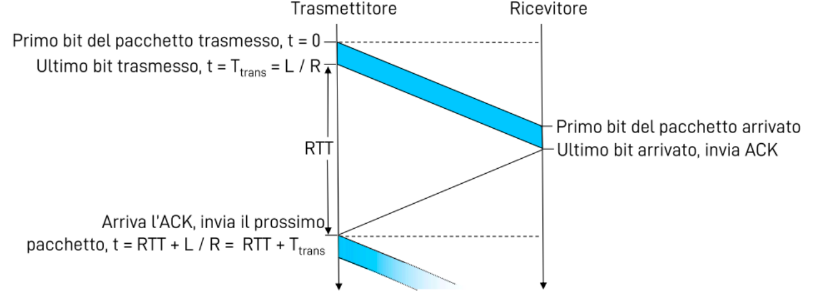
\includegraphics[width=\textwidth]{schema-stop-and-wait.png}
    \caption{Funzionamento protocollo \emph{Stop-and-Wait}}
\end{figure}
\begin{note}
    Nel calcolo del tempo $t$ si è assunta come trascurabile la durata del
    pacchetto \emph{ACK}.
\end{note}

\paragraph{Efficienza}
Se assumiamo $\hyperlink{sym:2}{R}=1Gbit/s$, $\hyperlink{sym:5}{RTT}=30ms$ e
$\hyperlink{sym:1}{L}=8000bit$, il \nameref{ssec:num1} vale $d_{trasferimento}=
\frac{L}{R}=8\mu s$. Quindi, il \emph{throughput} percepito a livello applicazione
è:
\[\emph{Throughput}=\frac{L}{d_{trasferimento}+RTT}=\frac{8000bit}{0.008ms+30ms}=33kByte/s\]
L'efficienza invece, vale:
\[\emph{Efficienza}=\frac{d_{trasferimento}}{d_{trasferimento}+RTT}=0.00027=0.027\%\]
Dai calcoli risulta evidente l'enorme inefficienza di questo protocollo, dovuta
al fatto che per la maggior parte del tempo gli \emph{host} restano in attesa.

\paragraph{Pipelining}
Con la tecnica del \emph{pipelining} il mittente invia più pacchetti alla volta
e tiene traccia del loro numero di sequenza.

\begin{figure}[h!]
    \centering
    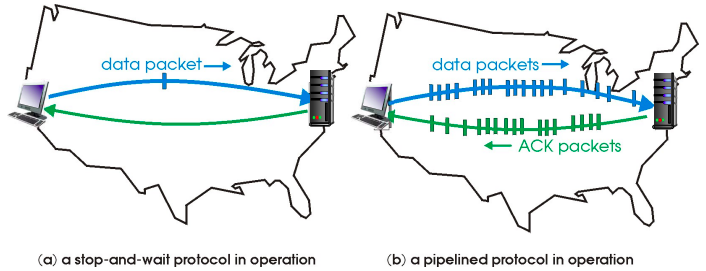
\includegraphics[width=\textwidth]{stop-and-wait-vs-pipelining.png}
    \caption{\emph{Stop-and-Wait} e protocollo con \emph{pipelining}}
\end{figure}\noindent
L'utilizzo del \emph{pipelining} permette di aumentare il \emph{throughput} di un
collegamento. Se, per esempio, si applica il \emph{pipelining} al protocollo
\emph{Stop-and-Wait}, permettendogli quindi di inviare 3 pacchetti prima di
mettersi in attesa, si triplica il \emph{throughput}.

\newpage
\begin{figure}[ht]
    \centering
    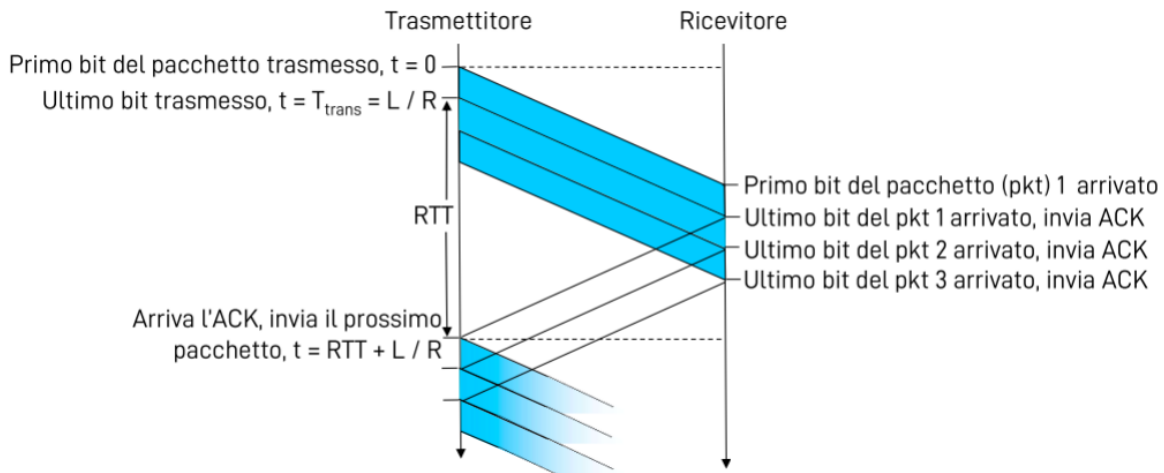
\includegraphics[width=\textwidth]{stop-and-wait-pipelining.png}
    \caption{Funzionamento protocollo \emph{Stop-and-Wait} con \emph{pipelining}}
\end{figure}\noindent
Ricalcolando il \emph{throughput} si può vedere come risulti effettivamente
triplicato:
\[\emph{Throughput}=\frac{3L}{d_{trasferimento}+RTT}=100kByte/s\]
In generale, il \emph{throughput} aumenta di tante volte quanti sono i pacchetti
trasmessi prima della messa in attesa. Tuttavia, ciò vale fino a quando il tempo
necessario a trasmettere quei pacchetti rimane inferiore al \emph{RTT}.

\subsection{Finestre di trasmissione e acknowledgement}
\paragraph{Finestre di trasmissione}
Il numero di pacchetti trasmesso prima della messa in attesa, viene detto
\quotes{\emph{dimensione della finestra}}. Diamo quindi le seguenti definizioni:
\begin{definition}[Finestra di trasmissione - \bm{$W_T$}]
    La finestra di trasmissione, indicata in simboli come $W_T$, è l'insieme di
    PDU che il mittente può trasmettere senza avere ancora ricevuto l'ACK
    corrispondente. La dimensione massima della finestra è limitata dalla
    quantità di memoria allocata dal trasmettitore ed è indicata in simboli come
    $|W_T|$.
\end{definition}
\begin{definition}[Finestra di ricezione - \bm{$W_R$}]
    La finestra di ricezione, indicata in simboli come $W_R$, è l'insieme di
    PDU che il destinatario può ricevere e memorizzare. La dimensione massima
    della finestra è limitata dalla quantità di memoria allocata dal ricevitore.
\end{definition}
\begin{definition}[Puntatore low - \bm{$W_{LOW}$}]
    Il puntatore low, indicato in simboli come $W_{LOW}$, è un puntatore al
    primo pacchetto della finestra di trasmissione $W_T$.
\end{definition}
\newpage
\begin{definition}[Puntatore up - \bm{$W_{UP}$}]
    Il puntatore up, indicato in simboli come $W_{UP}$, è un puntatore
    all'ultimo pacchetto già trasmesso e potrebbe non coincidere con l'ultimo
    pacchetto della finestra di trasmissione.
\end{definition}

\begin{figure}[ht]
    \centering
    \subfloat[\emph{Finestra di trasmissione}]{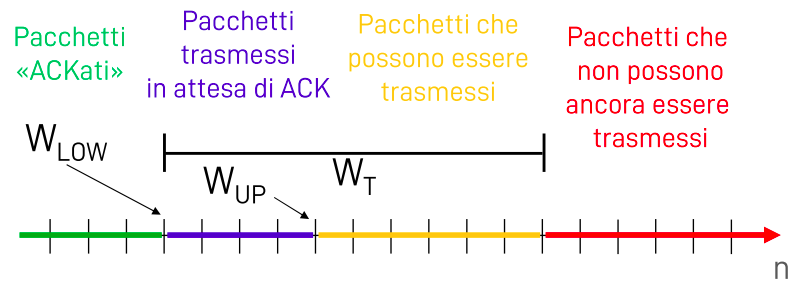
\includegraphics[width=0.8\textwidth]{finestra-trasmissione.png}}
    \hfill
    \subfloat[\emph{Finestra di ricezione}]{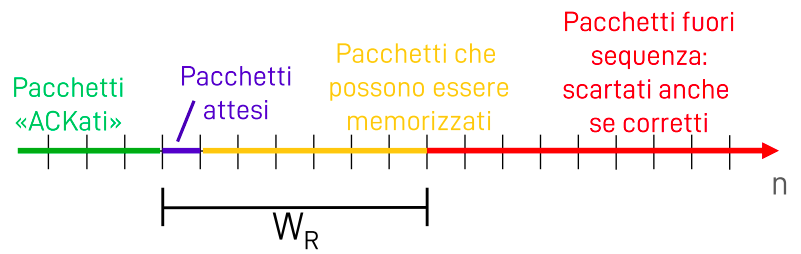
\includegraphics[width=0.8\textwidth]{finestra-ricezione.png}}
    \caption{\emph{Finestre di trasmissione} e \emph{ricezione}}
\end{figure}

\paragraph{Pacchetti di acknowledgement}
Finora abbiamo parlato dei pacchetti \emph{\gls{glos:ACK}} senza specificare
alcun tipo di dettaglio, ma in realtà esistono molteplici tipi di
\emph{acknowledgement}:
\begin{itemize}
    \item \emph{ACK individuale}: indica la corretta ricezione di un pacchetto
    specifico. $ACK(n)$ significa che è stato ricevuto il pacchetto $n$;
    \item \emph{ACK cumulativo}: indica la corretta ricezione di tutti i
    pacchetti fino ad un certo indice. $ACK(n)$ significa che sono stati
    ricevuti correttamente tutti i pacchetti fino al pacchetto $n$ (escluso);
    \item \emph{ACK negativo} (\emph{NACK}): richieda la ritrasmissione di un
    singolo pacchetto. $\emph{NACK}(n)$ significa che il pacchetto $n$ deve
    essere ritrasmesso.
\end{itemize}
Con la tecnica del \quotes{\emph{Piggybacking}} è possibile inserire un
\emph{ACK} in un pacchetto dati.

\subsection{Protocollo Go-back-N}
Nel protocollo \emph{Go-back-N} il mittente può avere fino a $N$ pacchetti
senza \emph{ACK} in pipeline. Il destinatario comunica la corretta ricezione dei
pacchetti mediante \emph{ACK cumulativi} e nel caso di pacchetti non ricevuti non
trasmette alcun \emph{ACK}. Fino a quando non verrà ricevuto il pacchetto mancante,
il protocollo continuerà a scartare tutti i successivi pacchetti ricevuti e, per
ognuno, ritrasmetterà l'ultimo \emph{ACK} inviato.

Il mittente ha un timer per il più vecchio pacchetto non confermato e quando
scade ritrasmette tutti i pacchetti per i quali non ha ricevuto \emph{ACK}.

Per la natura degli \emph{ACK cumulativi}, alcuni dei pacchetti ritrasmessi
potrebbero essere già stati ricevuti e scartati in precedenza. Questo protocollo
soffre quindi di un'inefficienza intrinseca.

\begin{figure}[h!]
    \centering
    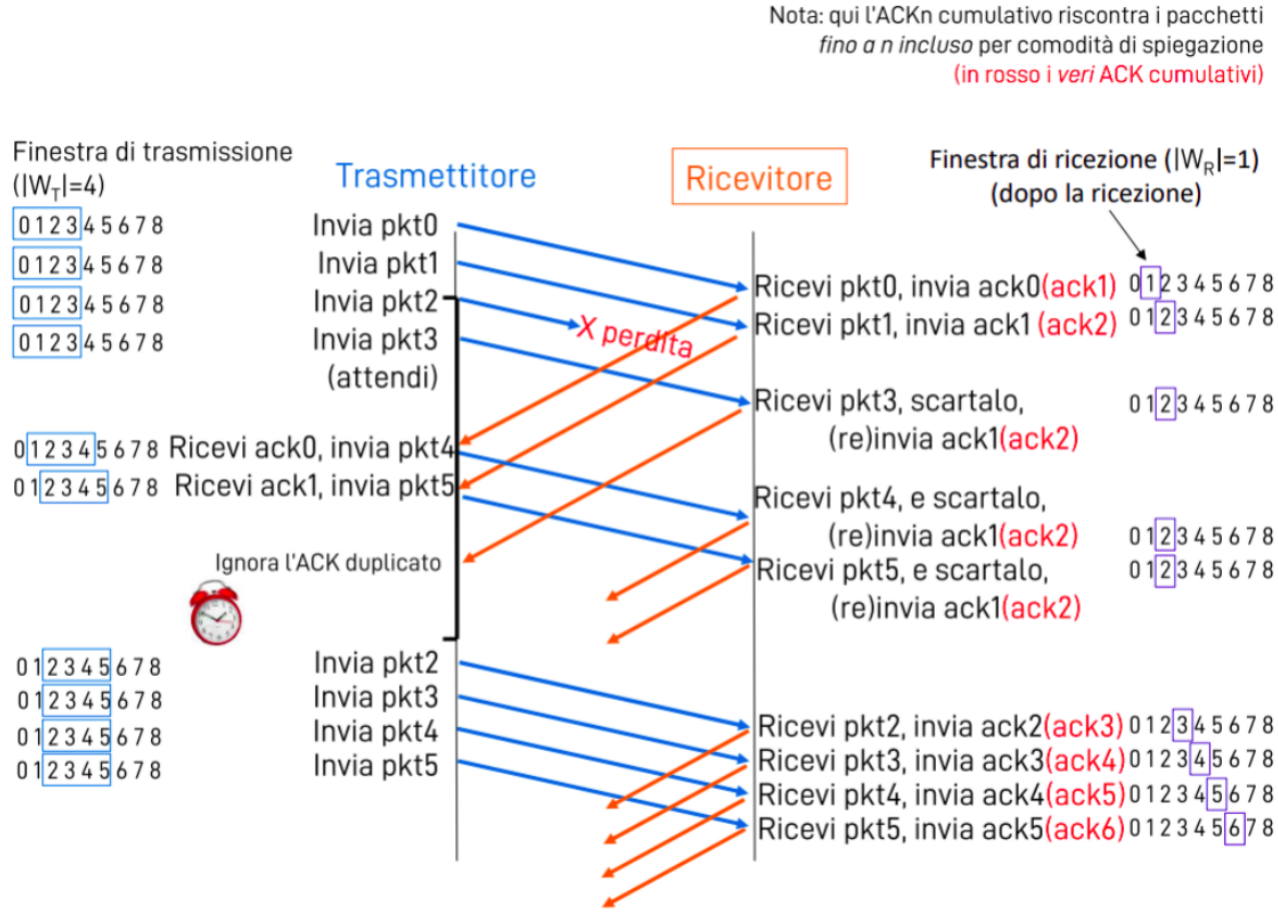
\includegraphics[width=\textwidth]{go-back-n.png}
    \caption{Funzionamento protocollo \emph{Go-back-N}}
\end{figure}\noindent
Ogni volta che il destinatario riceve un pacchetto e trasmette l'\emph{ACK},
quel pacchetto viene trasferito all'applicazione del ricevitore.

\subsection{Protocollo Selective repeat}
Come nel \emph{Go-back-N}, il mittente può avere fino a $N$ pacchetti senza
\emph{ACK}, ma diversamente da prima, il ricevente invia \emph{ACK individuali}.
Il mittente mantiene un timer per ciascun pacchetto non confermato e quando
scade ritrasmette il pacchetto associato a quel timer.

Un'altra differenza col \emph{Go-back-N} è che nel \emph{Selective repeat},
quando viene ricevuto un pacchetto successivo ad un pacchetto mancante, non
viene scartato, ma viene salvato in un buffer.

\begin{figure}[ht]
    \centering
    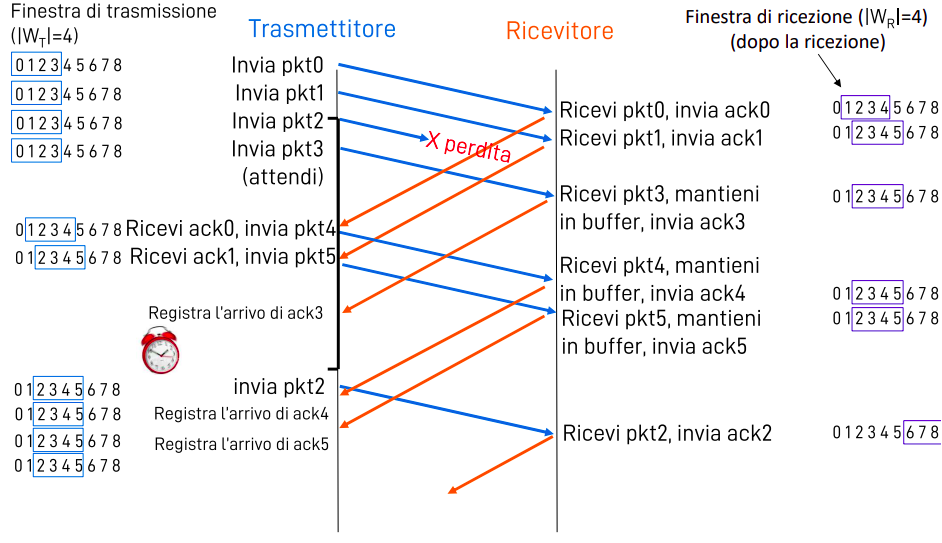
\includegraphics[width=\textwidth]{selective-repeat.png}
    \caption{Funzionamento protocollo \emph{Selective repeat}}
\end{figure}
\bigskip\noindent
Come prima, i pacchetti vengono consegnati all'applicazione del ricevitore ogni
volta che l'\emph{ACK} ad essi associato viene trasmesso. Nel caso di pacchetti
persi, quando questi vengono ricevuti, vengono inviati all'applicazione ricevente
il pacchetto appena arrivato e tutti quelli successivi che erano stati salvati
nel buffer.

\paragraph{Relazione tra numeri dimensione della finestra e numeri di sequenza}
Nel protocollo \emph{Selective repeat}, il numero di sequenza dei pacchetti è
ciclico, cioè, se vengono usati $k$ bit per codificare il numero di sequenza,
si avrà un periodo, ovvero una quantità di numeri di sequenza, pari a $2^k$.

Fissato $k$, la dimensione totale delle \emph{finestre di trasmissione} e
\emph{ricezione} deve esser minore o uguale a $2^k$, ovvero deve valere:
\[W_T+W_R\leq2^k\]
Nel caso particolare in cui $W_T=W_R$ deve valere:
\[W_T\leq2^{k-1}=\frac{2^k}{2}\]
Il motivo per il quale deve sussistere questa condizione è che, in questo modo,
i numeri di sequenza delle \emph{finestre di trasmissione} e di \emph{ricezione}
non potranno mai sovrapporsi. La sovrapposizione va evitata perché altrimenti
potrebbe accadere che il ricevente riconosca come pacchetti nuovi pacchetti che
in realtà sono già stati ricevuti.
\paragraph{Esempio di sovrapposizione}
In questo esempio, i numeri di sequenza sono codificati su 2 bit e le
\emph{finestre} hanno entrambe dimensione $3$, per cui $W_T+W_R=6>2^2=4$.

Vengono inviati e correttamente ricevuti i primi tre pacchetti. Di conseguenza,
la \emph{finestra di ricezione} viene shiftata tre volte e, alla fine, rimane
in attesa dei pacchetti con numeri $3$, $0$ e $1$. Tuttavia, se accade che
tutti e tre gli \emph{acknowledgement} vengono persi durante la trasmissione, il
mittente, non ricevendo nessuna conferma di ricezione, provvede ad impostare un
timer per ciascuno di essi.

Allo scadere del primo timer, il mittente ritrasmette il pacchetto con numero di
sequenza $0$ nella \emph{finestra di trasmissione}. Il destinatario lo riceve e,
poiché nella sua \emph{finestra di ricezione} è presente un pacchetto con numero
$0$, accetta il pacchetto ricevuto e trasmette un \emph{ACK}. Il problema è che
quel pacchetto in realtà era già stato ricevuto, quindi il ricevente si è
ritrovato con un pacchetto duplicato.

\begin{figure}[ht]
    \centering
    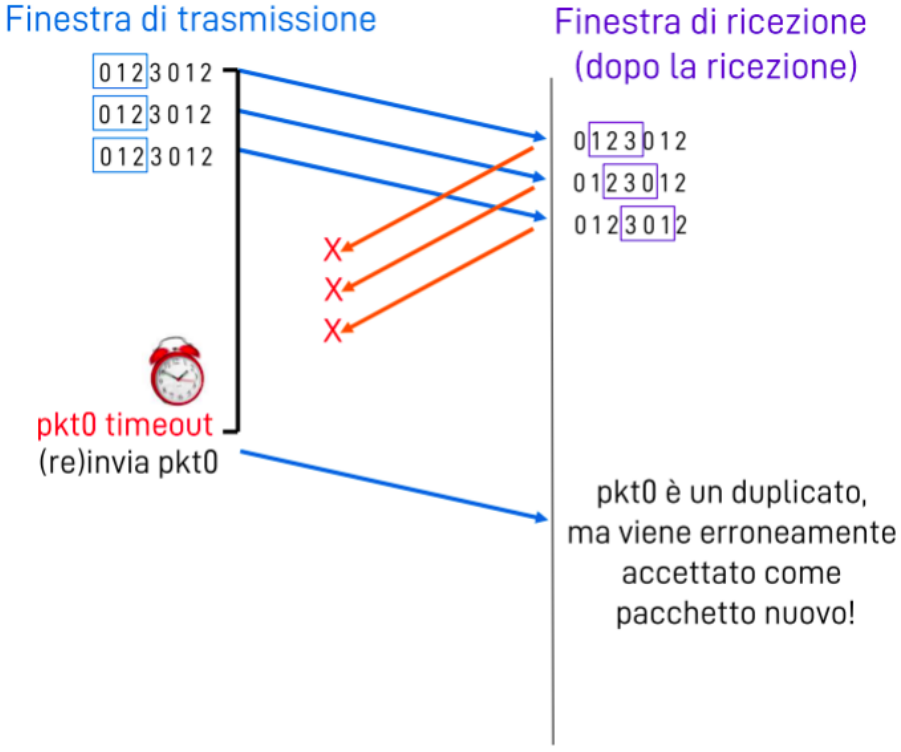
\includegraphics[width=0.8\textwidth]{selective-repeat-problema-num-seq.png}
    \caption{Esempio sovrapposizione numeri di sequenza nel \emph{Selective repeat}}
\end{figure}

\begin{note}
    Nel protocollo \emph{Go-back-N}, la condizione sui numeri di sequenza e sulle
    dimensioni delle finestre non vale, in quanto, il ricevente trasmette
    \emph{ACK cumulativi} e non shifta la \emph{finestra di ricezione} finché non
    riceve una sequenza completa di pacchetti.
    Di conseguenza, se i numeri di sequenza fossero codificati su $k$ bit e la
    \emph{finestra di trasmissione} avesse dimensione $2^k-1$, nell'ipotesi in
    cui tutti i pacchetti trasmessi venissero ricevuti, ma andassero persi tutti
    gli \emph{ACK}, se anche il mittente ritrasmettesse un pacchetto già
    ricevuto dal destinatario, questo lo scarterebbe poiché nella sua
    \emph{finestra di ricezione} quel numero di sequenza non ci sarebbe più.
\end{note}

\section{Protocollo TCP}
Il protocollo \emph{\gls{prot:TCP}} è un protocollo connesso che consente a due
\emph{host} di scambiarsi \emph{segmenti} in modo affidabile e ordinato. In
particolare, i \emph{segmenti TCP} viaggiano all'interno di una connessione
\emph{full duplex} che consente trasmissioni in entrambe le direzioni.

Il \emph{TCP} fa uso del \emph{pipelining}, quindi esistono \emph{finestre di
trasmissione e ricezione} la cui dimensione viene stabilita in base a meccanismi
di \emph{controllo di flusso} e \emph{congestione} e quindi varia nel tempo.

\paragraph{Struttura dei segmenti TCP}
Proprio per le garanzie offerte dal \emph{TCP}, la struttura dei \emph{segmenti}
è più complicata rispetto a quanto visto con i \emph{segmenti UDP}.

\begin{figure}[ht]
    \centering
    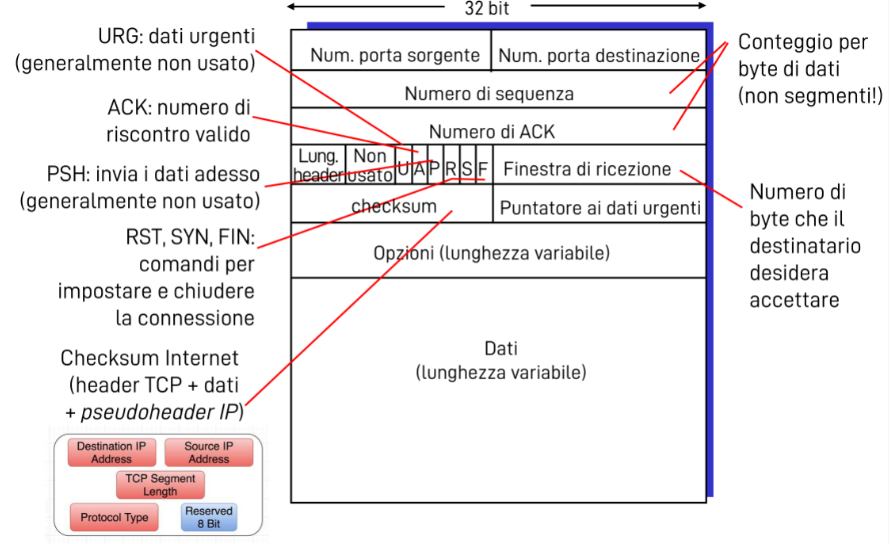
\includegraphics[width=0.75\textwidth]{struttura-messaggi-tcp.png}
    \caption{Struttura di un \emph{segmento TCP}}
\end{figure}
La dimensione della \emph{finestra di ricezione} indicata nel campo
\emph{\gls{glos:RWND}}\footnote{Nella figura si fa riferimento al campo
\texttt{Finestra di ricezione}}, è rappresentata da un valore a 16 bit,
che definisce il numero di byte che il destinatario può memorizzare. Di
conseguenza, rappresenta anche la massima quantità di dati che può essere
in transito durante un \emph{RTT}.

\noindent
Poiché \emph{RWND} è un valore a 16 bit, possono transitare contemporaneamente
$64kByte$. Tuttavia, è possibile aumentare quel limite usando un meccanismo di
\emph{scalatura}, cioè decidendo che quel valore non rappresenta il numero di
byte, ma un loro multiplo.

I campi \texttt{numero di sequenza} e \texttt{numero di ACK} indicano
rispettivamente il numero del primo byte di quel segmento all'intero del
\emph{flusso di dati} e il numero di sequenza del prossimo byte atteso dall'altro
lato, ricordando che il \emph{TCP} utilizza \emph{ACK cumulativi}.

\begin{note}
    Per quanto riguarda la gestione dei \emph{segmenti} fuori sequenza, il
    \emph{TCP} non stabilisce una policy unica, ma dipende dall'implementazione.
\end{note}

\begin{figure}[h!]
    \centering
    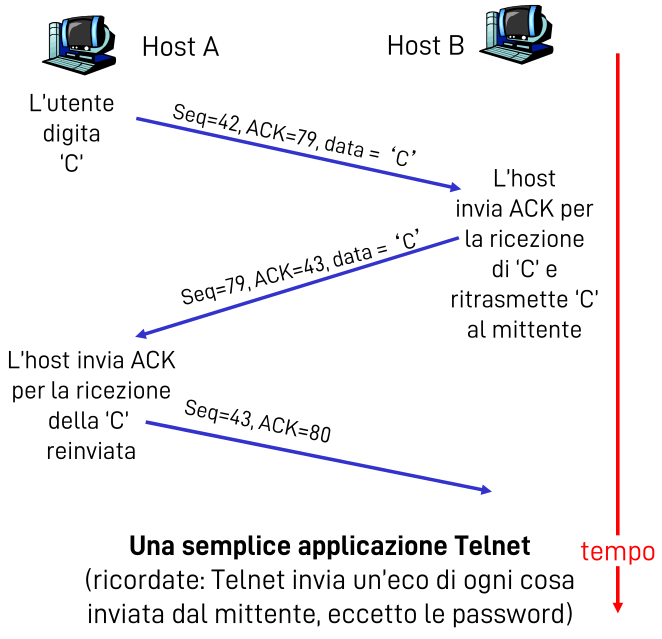
\includegraphics[width=0.55\textwidth]{tcp-esempio-telnet.png}
    \caption{\emph{Numeri di sequenza} e \emph{ACK} in una comunicazione \emph{TCP}}
\end{figure}

\subsection{Instaurazione di una connessione TCP}
Una connessione \emph{TCP} viene instaurata mediante un meccanismo detto
\emph{Three-way handshake}:
\begin{enumerate}
    \item L'\emph{host A} inizia la connessione, quindi, invia all'\emph{host B}
    un \emph{segmento} con flag \texttt{SYN} impostato a $1$, porta sorgente pari
    ad $A$, porta destinazione $B$ e numero di sequenza iniziale $x$;
    \item L'\emph{host B} riceve il \emph{segmento} di inizializzazione e risponde
    con un \emph{segmento} nel quale i flag \texttt{SYN} e \texttt{ACK} sono
    impostati a $1$, le porte sorgente e destinazione sono rispettivamente $B$
    ed $A$, il numero di sequenza iniziale è $y$ e il numero di \emph{ACK} $x+1$;
    \item L'\emph{host A} risponde inviano un \emph{segmento ACK} con porta
    sorgente $A$, destinazione $B$ e numero di \emph{ACK} $y+1$;
\end{enumerate}
\begin{figure}[h!]
    \centering
    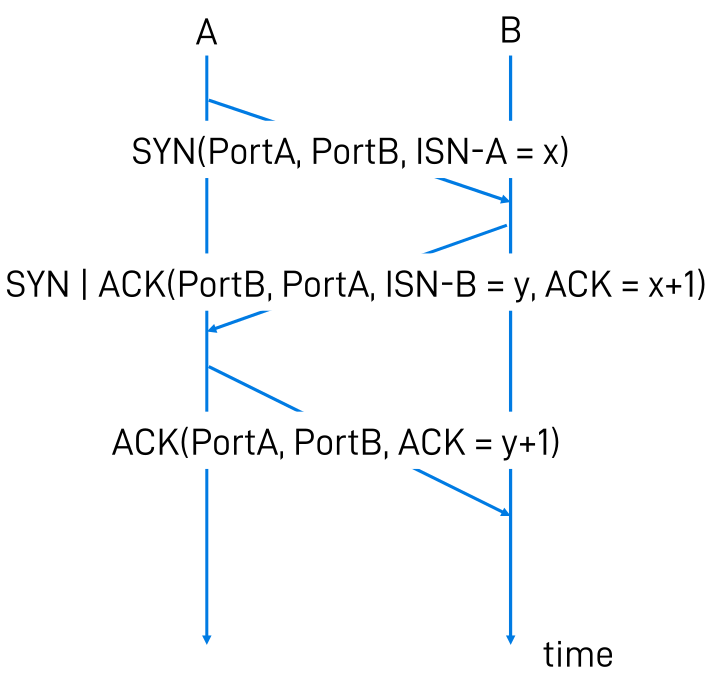
\includegraphics[width=0.6\textwidth]{tcp-three-way-handshake.png}
    \caption{Meccanismo di \emph{Three-way handshake} nel \emph{TCP}}
\end{figure}
\begin{note}
    \emph{ISN} sta per \emph{Initial Sequence Number} ed è il numero di
    partenza dei numeri di sequenza che non iniziano necessariamente da
    zero.
\end{note}

\subsection{Dimensione dei segmenti}
Sebbene il protocollo \emph{TCP} gestisca i dati organizzandoli byte, non invia
mai singoli byte, ma cerca di accorparli in un unico \emph{segmento} di dimensione
massima\footnote{Il \emph{TCP} può essere costretto ad inviare singoli byte}.

L'\emph{\gls{glos:MSS}} dipende da un parametro del \emph{livello} sottostante,
il \emph{livello Rete}, che si chiama \emph{\gls{glos:MTU}}, il quale a sua
volta dipende dall'\emph{MTU} del \emph{livello Data Link}. Tutti questi parametri
dipendono anche dalle specifiche dei collegamenti attraverso i quali dovranno
transitare i dati.

Comunque, l'\emph{MSS} indica la dimensione massima del \emph{payload}, cioè i
dati trasportati dal \emph{segmento}. Tuttavia, poiché non esistono meccanismi
per la negoziazione di questo parametro, il \emph{TCP} procede per
tentativi, andando progressivamente ad incrementarlo fino a quando non viene
perso qualche \emph{segmento} o non viene ricevuta una comunicazione esplicita di
incompatibilità\footnote{Non viene inviata sempre, dipende dalla configurazione
dei singoli \emph{host}}.

Di default, l'\emph{MSS} viene impostata a 1460 byte (1500 byte per l'\emph{MTU}
del \emph{livello Data Link} e 40 byte per gli \emph{header TCP} e \emph{IP}).

In ogni caso, esiste una dimensione minima fissata a 536 byte dovuta al fatto
che il protocollo \emph{\gls{prot:IP}} richiede una \emph{MTU} minima
di 576 byte (536 byte per il \emph{payload} e 40 byte di \emph{header}).

\subsection{Chiusura di una connessione TCP}
Poiché le connessioni \emph{TCP} sono bidirezionali, al termine della comunicazione,
vanno chiuse in entrambe le direzioni. Esistono due modalità di terminazione:
una cosiddetta \quotes{gentile} e una \quotes{brusca}.

\paragraph{Modalità \quotes{gentile}}
L'\emph{host} che intende terminare la connessione invia un \emph{segmento} nel
quale il flag \texttt{FIN} è impostato a 1 e il ricevitore risponde con un \emph{ACK}.
A questo punto la connessione è chiusa per metà, in quanto il primo \emph{host}
non può più trasmettere nulla, ad eccezione degli \emph{acknowledgement}, mentre
il secondo può continuare ad inviare \emph{segmenti}.

Per terminare del tutto la connessione è necessario che anche il secondo
\emph{host} invii un \emph{segmento} con flag \texttt{FIN} a 1.

\begin{figure}[h!]
    \centering
    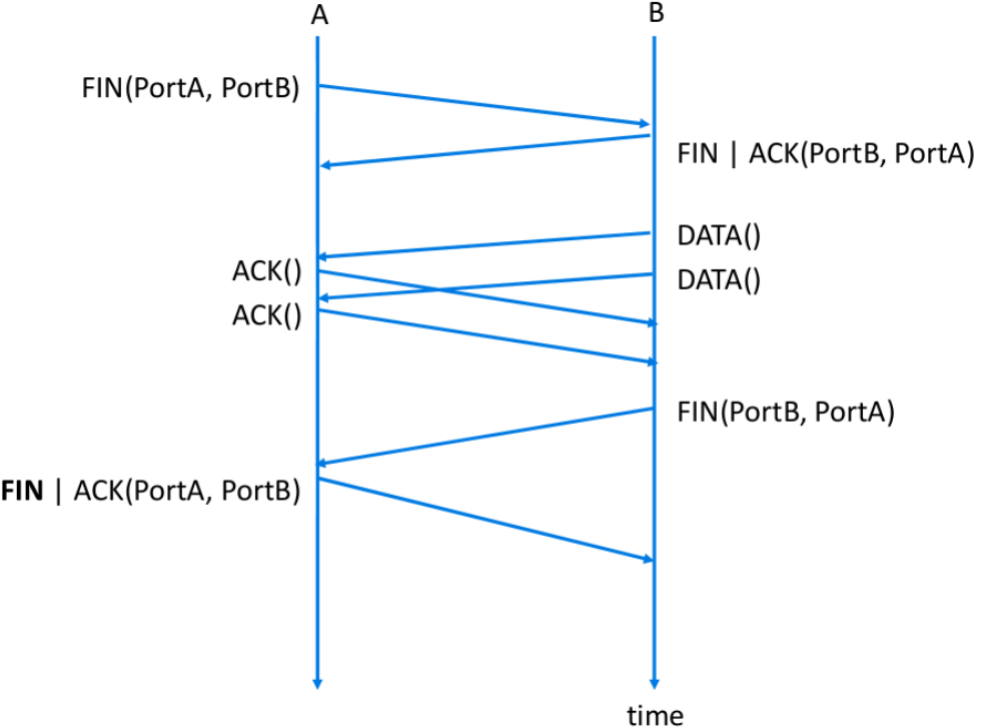
\includegraphics[width=0.8\textwidth]{tcp-chiusura-gentile.png}
    \caption{Chiusura \quotes{gentile} di una connessione \emph{TCP}}
\end{figure}

\paragraph{Modalità \quotes{brusca}}
Questa modalità viene usata per resettare connessioni non più gestibili o
che si trovano in uno stato di errore (e.g. viene ricevuto un \emph{ACK} su una
connessione mai aperta). Per farlo, uno degli \emph{host} invia un
\emph{segmento} con flag \texttt{RST} impostato a 1. Quindi, entrambi gli
\emph{host} liberano le risorse allocate dal sistema operativo per quella
connessione.

\begin{note}
    I server possono usare questa tecnica per chiudere velocemente le
    connessioni con i client.
\end{note}

\begin{figure}[ht]
    \centering
    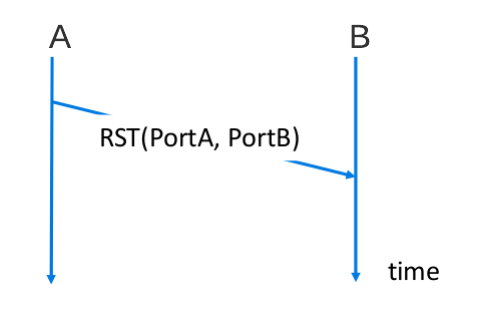
\includegraphics[width=0.4\textwidth]{tcp-chiusura-brusca.png}
    \caption{Chiusura \quotes{brusca} di una connessione \emph{TCP}}
\end{figure}

\subsection{Stimare l'RTT e scegliere l'RTO}
La scelta dell'\emph{\gls{glos:RTO}}, ovvero la durate dei timer, influenza le
prestazioni della comunicazione. Se viene scelto un valore troppo piccolo, c'è
il rischio vengano effettuate delle ritrasmissioni non necessarie, mentre al
contrario, un valore troppo grande rende il \emph{TCP} troppo poco reattivo
alle perdite. In ogni caso, l'\emph{RTO} deve essere maggiore
dell'\emph{\gls{glos:RTT}}, che però è soggetto a variazioni.

\begin{definition}[SampleRTT]
    Il sampleRTT è il tempo misurato dalla trasmissione di un segmento alla
    ricezione del relativo ACK, ignorando le ritrasmissioni.
\end{definition}\noindent
Poiché il \emph{sampleRTT} è diverso per ogni \emph{segmento}, viene realizzata
una stima partendo dalla media dei precedenti valori di \emph{sampleRTT}\footnotemark.
\footnotetext{Si effettua una media pesata che da maggiore peso ai valori più
recenti e progressivamente meno peso a quelli più vecchi.}
Il tempo stimato viene calcolato, partendo dalla stima precedente, mediante una
\emph{media mobile esponenziale ponderata} e, in particolare, vale la seguente
formula:
\[\emph{EstimatedRTT}=(1-\alpha)\cdot\emph{EstimatedRTT}+\alpha\cdot
\emph{SampleRTT}\quad\text{per }\alpha=0.125\]
Con questo tipo di formula, il peso dei campioni precedenti diminuisce
esponenzialmente.

A questo punto, l'\emph{RTO} può essere definito pari alla stima dell'\emph{RTT}
con in aggiunta un margine di sicurezza. Per fare ciò, bisogna innanzitutto
sapere di quanto il valore stimato per l'\emph{RTT} si discosta da quello reale:
\[\emph{DevRTT}=(1-\beta)\cdot\emph{DevRTT}+\beta\cdot|\emph{SampleRTT}-
\emph{EstimatedRTT}\,|\quad\text{per }\beta=0.25\]
Anche in questo caso, la deviazione viene calcolata a partire dal valore precedente.
Il \emph{DevRTT} costituisce il valore di partenza per la definizione del margine
di sicurezza. Noto ciò, l'\emph{RTO} è definito come:
\[\emph{RTO}=\emph{EstimatedRTT}+4\emph{DevRTT}\]

\begin{figure}[ht]
    \centering
    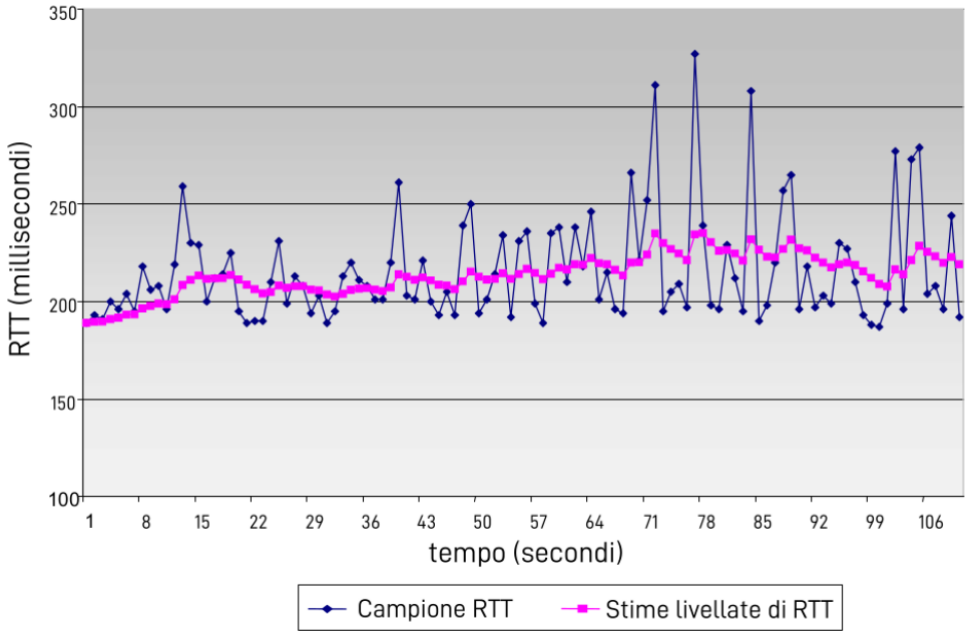
\includegraphics[width=0.8\textwidth]{tcp-stima-rtt.png}
    \caption{Confronto tra \emph{RTT} reale e stimato}
\end{figure}

\paragraph{Inizializzazione dei valori}
Ovviamente, all'avvio della comunicazione \emph{EstimatedRTT} e \emph{DevRTT}
non sono definiti, quindi devono essere inizializzati a un qualche valore. Lo
standard stabilisce che quando si è in possesso di una sola misura di \emph{RTT},
si pongono $\emph{EstimatedRTT}=\emph{SampleRTT}$ e $\emph{DevRTT}=\emph{SampleRTT}/2$.
L'\emph{RTO} viene invece inizializzato a un secondo. Col procedere della
comunicazione i valori verranno progressivamente affinati.

\subsection{Controllo di flusso}
Il \emph{\nameref{def:7}}, come già accennato, è una delle funzionalità
offerte dal protocollo \emph{TCP} e permette al ricevitore di controllare la
velocità di trasmissione del mittente in modo da evitare di sovraccaricarsi.

Per farlo, il ricevitore comunica al mittente la quantità di spazio ancora
disponibile nel proprio buffer di ricezione e lo fa, indicando nell'\emph{header}
di ogni \emph{segmento} il valore della \emph{RWND}. Il mittente, quindi, limita
la propria \emph{finestra di trasmissione} al valore indicatogli dal ricevente.

Questa scelta garantisce che il buffer del destinatario non andrà mai in
overflow costringendolo a scartare i \emph{segmenti} ricevuti per mancanza di
spazio.

\begin{figure}[h!]
    \centering
    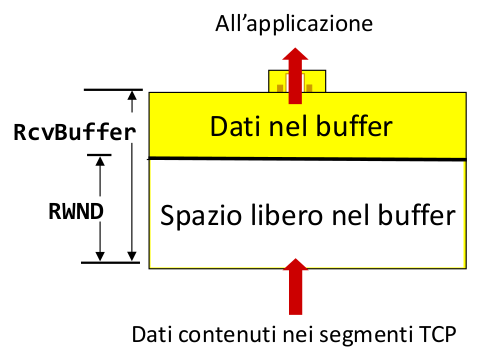
\includegraphics[width=0.5\textwidth]{buffering-al-ricevitore-tcp.png}
    \caption{Gestione del buffer di ricezione}
\end{figure}
\newpage
\begin{figure}[ht!]
    \centering
    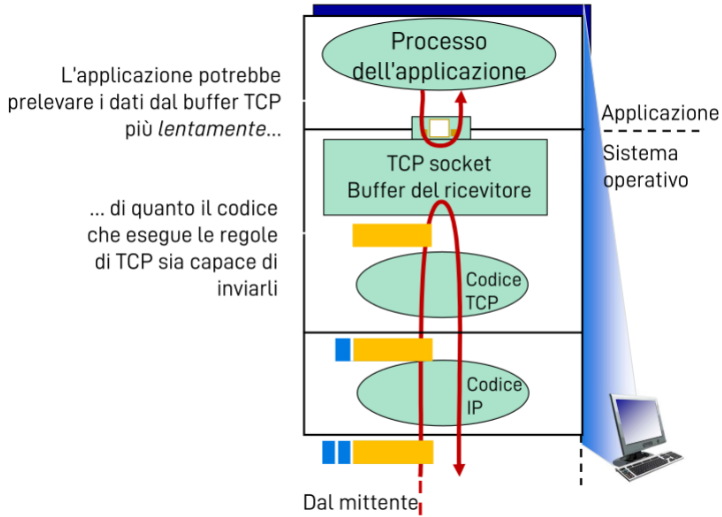
\includegraphics[width=0.6\textwidth]{controllo-flusso-tcp.png}
    \caption{Gestione dello \emph{stack protocollare} al ricevitore}
\end{figure}

\section{Gestione della congestione}
Abbiamo già dato una definizione di \nameref{def:6}, ma informalmente possiamo
dire che la \emph{congestione} si verifica quando troppi trasmettitori stanno
inviando troppi dati e la rete non è in grado di gestire tutto quel traffico.
Una rete congestionata comporta la perdita di \emph{pacchetti}, dovuta
all'overflow dei buffer nei \emph{router}, e lunghi ritardi nel trasferimento,
dovuti all'accodamento dei \emph{pacchetti} nei buffer.

\subsection{Modelli per sistemi a coda}
Un \emph{sistema a coda} comprende una \quotes{fila d'attesa}, realizzata
solitamente con una \emph{coda}, e un \emph{server}. I parametri presi in
considerazione sono due:
\begin{enumerate}
    \item \emph{Tasso di arrivo $\lambda$}: è il numero medio di \emph{pacchetti},
    o in generale di \emph{unità di lavoro}, che entrano nella \emph{coda} per
    unità di tempo;
    \item \emph{Tasso di servizio $\mu$}: è il tempo medio richiesto dal
    \emph{server} per trasmettere un \emph{pacchetto}, o in generale per concludere
    un lavoro;
\end{enumerate}\noindent
Gli \emph{arrivi} e i \emph{tempi di servizio} sono distribuiti secondo
distribuzioni statistiche. Ad esempio, nei \emph{sistemi a coda} di tipo
$M/M/1$\footnotemark, gli \emph{arrivi} sono distribuiti come $exp\left(\frac{1}
{\lambda}\right)$, i \emph{tempi di servizio} come $exp\left(\frac{1}{\mu}\right)$
e c'è un solo \emph{server} a ricevere i \emph{pacchetti}.
\footnotetext{$M$ sta per \emph{Markovian} e si riferisce alla distribuzione
esponenziale.}

\begin{figure}[h!]
    \centering
    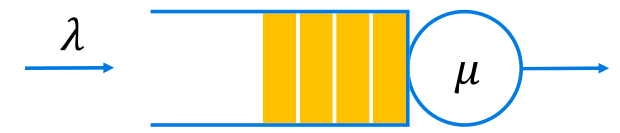
\includegraphics[width=0.8\textwidth]{sistemi-a-coda.png}
    \caption{Schema di un \emph{sistema a coda}}
\end{figure}\noindent
Le proprietà dei \emph{sistemi a coda} possono essere calcolate analiticamente.
Ad esempio, nei \emph{sistemi} $M/M/1$ si ha che:
\begin{itemize}
    \item \emph{Carico del server}: $\rho=\frac{\lambda}{\mu}$;
    \item \emph{Lunghezza media della coda}: $L=\frac{\rho^2}{1-\rho}$ per $\rho<1$;
    \item \emph{Probabilità che in un qualunque momento ci siano $n$ pacchetti in
    coda}: $\pi_n=(1-\rho)\cdot\rho^n$;
\end{itemize}
Poiché $\lambda$ e $\mu$ sono medie statistiche e non delle costanti, i dati
reali non coincidono sempre con quelli stimati. Inoltre, la probabilità che i
\emph{pacchetti} si accodino, anche se molto piccola, non è mai nulla.

\subsection{Cause della congestione}
Vediamo ora come si manifesta la \emph{congestione} in alcuni scenari.
\paragraph{Scenario 1}
Si supponga di avere due trasmettitori e due ricevitori e che i dati debbano
passare per un \emph{router} con un buffer infinito. Se la \hyperlink{sym:2}
{\emph{capacità del link}} di uscita è $R$ e non ci sono ritrasmissioni, il
\emph{throughput} massimo è $\frac{R}{2}$. Inoltre, se il \emph{tasso}
$\lambda_{in}$ si avvicina a $\frac{R}{2}$ si avrà a che fare con lunghi ritardi.

\begin{figure}[h!]
    \centering
    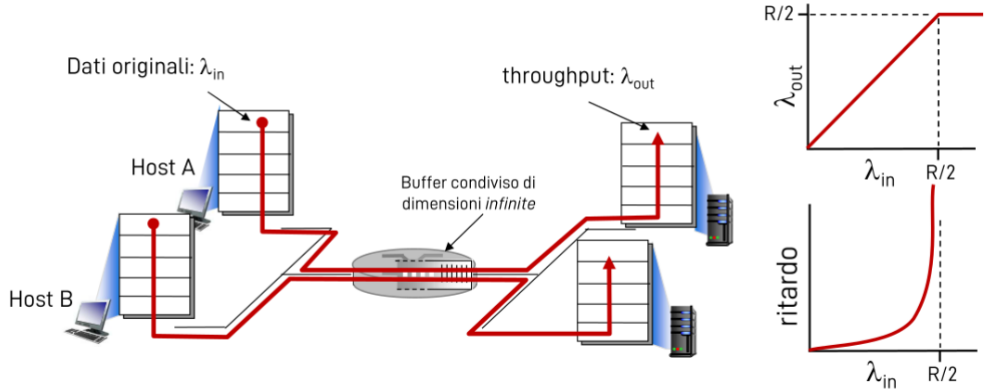
\includegraphics[width=0.8\textwidth]{congestione-scenario-1.png}
    \caption{\emph{Congestione} - scenario 1}
\end{figure}

\paragraph{Scenario 2}
Si supponga di avere un \emph{router} con un buffer di dimensione finita e che il
mittente ritrasmetta i pacchetti finiti in timeout. Si indichi con $\lambda_{in}$
il \emph{tasso di arrivo} dall'applicazione al mittente e con $\lambda_{out}$
il \emph{tasso} percepito dall'applicazione del destinatario.

Poiché il mittente ritrasmette i pacchetti persi, vengono inviati più dati di
quelli che si invierebbero se non ci fossero ritrasmissioni, di conseguenza se si
calcola il \emph{tasso di arrivo} al \emph{livello Trasporto}, e lo si indica con
$\lambda'_{in}$, si ha che $\lambda'_{in}>\lambda_{in}$, in quanto il \emph{livello
Trasporto} include anche tutte le ritrasmissioni.

In questo scenario possiamo distinguere due casi:
\begin{itemize}
    \item \emph{Caso ideale}: si ha una perfetta conoscenza della situazione e
    quindi il mittente può inviare dati solo quando sa che nel buffer del
    \emph{router} c'è spazio per riceverli;
    \item \emph{Caso realistico}: si ha una conoscenza limitata della rete e
    quando scatta un timeout, il mittente ritrasmette il \emph{pacchetto}
    associato, ma potrebbe accadere che vengano consegnate entrambe le copie
    causando un dimezzamento del \emph{throughput};
\end{itemize}\noindent
Nel \emph{caso realistico} è possibile ipotizzare cosa accadrebbe se il mittente
ritrasmettesse i \emph{pacchetti} solo quando è sicuro che questi siano andati
persi, per esempio impostando timer piuttosto lunghi. In questo modo si potrebbe
migliorare il \emph{throughput}, tuttavia, è comunque possibile che a causa della
\emph{congestione} anche i pacchetti ritrasmessi vengano persi.
\begin{figure}[ht!]
    \centering
    \subfloat[\emph{Caso ideale}]{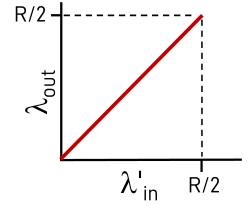
\includegraphics[width=0.3\textwidth]{congestione-scenario-2-caso-ideale.png}}
    \hfill
    \subfloat[\emph{Caso realistico}]{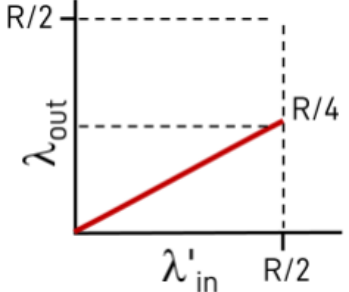
\includegraphics[width=0.3\textwidth]{congestione-scenario-2-caso-reale.png}}
    \hfill
    \subfloat[\emph{Caso realistico con certezza della perdita}]{\includegraphics[width=0.3\textwidth]{congestione-scenario-2-caso-reale-idealizzato.png}}
    \caption{\emph{Congestione} - scenario 2}
\end{figure}

\paragraph{Scenario 3}
Si supponga che siano possibili più percorsi e che i \emph{pacchetti} debbano
passare attraverso più di un \emph{router}. Se accade che $\lambda'_{in}$ e
$\lambda_{in}$ aumentano, la maggior parte, se non tutti, i \emph{pacchetti}
trasmessi vengono scartati portando $\lambda_{out}$ a 0.

\begin{figure}[h!]
    \centering
    \subfloat[Schema dello scenario]{\includegraphics[width=0.7\textwidth]{congestione-scenario-3.png}}
    \hfill
    \subfloat[Grafico del ritardo]{\includegraphics[width=0.28\textwidth]{congestione-scenario-3-grafico.png}}
    \caption{\emph{Congestione} - scenario 3}
\end{figure}

\begin{note}
    Ogni volta che un \emph{pacchetto} viene perso, tutte le risorse usate
    per portarlo fino a quel punto risultano sprecate.
\end{note}\noindent
In conclusione, possiamo affermare che con buffer infiniti non ci sono perdite, ma
se il \emph{tasso di invio} si avvicina troppo al \emph{tasso di servizio} i
ritardi si allungano di molto. Se i ritardi sono dovuti alla \emph{congestione}
provocata dalle ritrasmissioni fatte al termine di un timeout, si ha uno spreco
di risorse per via di ritrasmissioni inutili. Infine, se la \emph{congestione}
porta alla perdita dei \emph{pacchetti} si è costretti a pagare il costo della
loro ritrasmissione e lo sforzo richiesto per ridurre il tempo $\lambda'_{in}$
può provocare un crollo del \emph{throughput} vanificando così gli sforzi fatti.

\section{Controllo della congestione in TCP}
Il \emph{TCP} usa tecniche di \emph{controllo della congestione} per adattare
il \emph{tasso di trasmissione} alle condizioni della rete ed evitare di
congestionarla. Per fare ciò esistono diversi approcci:
\begin{itemize}
    \item \emph{Controllo di congestione end-to-end}: il livello di
    \emph{congestione} viene stimato tenendo traccia dei \emph{segmenti} persi
    e dei ritardi;
    \item \emph{Controllo di congestione assistito dalla rete}: i \emph{router}
    forniscono dei feedback agli \emph{host} sullo stato della rete
    (e.g. viene impostato un bit per indicare la \emph{congestione});
\end{itemize}
Non esiste un unico protocollo per il \emph{controllo della congestione}, ma
implementazioni diverse del \emph{TCP} adottano soluzione distinte.

\subsection{Protocollo AIMD}
Nel protocollo \emph{\gls{prot:AIMD}} il mittente aumenta progressivamente il
\emph{tasso di trasmissione}, cosa che coincide con l'aumento della dimensione
della \emph{finestra di trasmissione}, cercando di occupare tutta la banda
disponibile. Quando viene rilevata una perdita, la dimensione della \emph{finestra}
viene ridotta.

\bigskip\noindent
Questo protocollo è organizzato in due fasi:
\begin{itemize}
    \item \emph{Additive increase}: ad ogni \emph{\gls{glos:RTT}}, fino a quando
    non viene rilevata una perdita, la \emph{finestra di trasmissione} viene
    aumentata di una \emph{\gls{glos:MSS}};
    \item \emph{Multiplicative decrease}: quando viene rilevata una perdita, la
    \emph{finestra di trasmissione} viene dimezzata;
\end{itemize}

\begin{figure}[h!]
    \centering
    \includegraphics[width=0.9\textwidth]{tcp-aimd.png}
    \caption{Dimensione della \emph{finestra di trasmissione} in funzione del tempo}
\end{figure}

\begin{note}
    In realtà, più che di \emph{finestra di trasmissione} sarebbe meglio parlare
    di \emph{finestra di congestione}.
\end{note}
\begin{definition}[Finestra di congestione]
    La finestra di congestione è l'insieme delle PDU che possono essere
    inviate nella rete e la sua dimensione è definita in base alla quantità
    massima di dati che il mittente pensa di poter inviare senza sovraccaricare
    la rete.
\end{definition}\noindent
La dimensione della \emph{\gls{glos:CWND}} è soggetta a variazioni durante la
comunicazioni in quanto il valore viene deciso dinamicamente dall'algoritmo di
\emph{controllo della congestione}. Un'altra cosa che cambia durante la
comunicazione è la \emph{finestra di trasmissione}.

\begin{definition}[Finestra di trasmissione]
    La finestra di trasmissione è l'insieme delle PDU che possono essere inviate
    in rete senza saturare il ricevitore e la sua dimensione è definita come:
    \[|W_T|=\min(\emph{CWND},\,\emph{RWND})=\min(\emph{CWND},\,|W_R|)\]
\end{definition}

\paragraph{Fairness}
Il protocollo \emph{AIMD} permette di ottenere una distribuzione equa delle
risorse di rete. Ciò significa che se $k$ sessioni \emph{TCP} si dividono lo
stesso collegamento di banda $R$ che fa da collo di bottiglia, ogni sessione
dovrebbe percepire la stessa banda $\frac{R}{k}$. Questa caratteristica è
detta \emph{fairness}.

Ad esempio, se due connessioni stanno condividendo lo stesso collegamento,
nel corso del tempo, il processo di \emph{additive increase} fa aumentare la
\emph{banda} di entrambe le connessioni in modo lineare. D'altra parte, quando
si passa alla fase di \emph{multiplicative decrease}, la \emph{banda} viene
ridotta in modo proporzionale a quella che si stava utilizzando. Ciò significa
che la diminuzione sarà maggiore per la connessione che stava occupando la
fetta maggiore di \emph{banda}.

\begin{figure}[h!]
    \centering
    \includegraphics[width=0.7\textwidth]{tcp-aimd-fairness.png}
    \caption{Raggiungimento dello stato di \emph{fairness}}
\end{figure}

\paragraph{Slow Start e Congestion Avoidance}
L'algoritmo \emph{AIMD} suddivide la comunicazione in due fasi che si alternano:
\begin{itemize}
    \item \emph{Slow Start}: il mittente trasmette inizialmente un solo
    \emph{segmento} e, per ogni \emph{ACK} valido ricevuto, incrementa di una
    \emph{MSS} la \emph{CWND}, che quindi aumenta esponenzialmente la propria
    dimensione.

    Quando la \emph{CWND} raggiunge un valore soglia \emph{\gls{glos:SSTHRESH}}
    l'algoritmo passa in regime di \emph{Congestion Avoidance};
    \item \emph{Congestion Avoidance}: per ogni \emph{ACK} valido ricevuto, la
    \emph{CWND} aumenta di $MSS\cdot\frac{MSS}{CWND}$ byte ovvero $\frac{1}{CWND}$
    \emph{segmenti}. Ciò significa che per ogni \emph{RTT}, se vengono ricevuti
    tutti gli \emph{ACK} attesi (sono tanti quanto è la \emph{CWND}), la
    \emph{CWND} viene incrementata di una \emph{MSS} (un \emph{segmento}).
    In questa fase l'incremento della \emph{CWND} è lineare.
\end{itemize}

\begin{figure}[ht]
    \centering
    \includegraphics[width=\textwidth]{slow-start-ex.png}
    \caption{Crescita della \emph{CWND} in regime di \emph{slow start}}
\end{figure}
\newpage
\begin{figure}[h!]
    \centering
    \includegraphics[width=\textwidth]{congestion-avoidance-ex.png}
    \caption{Crescita della \emph{CWND} in regime di \emph{congestion avoidance}}
\end{figure}\noindent
Lavorando con l'\emph{AIMD} è possibile modificare le prestazioni della
comunicazione andando ad agire su quattro parametri:
\begin{itemize}
    \item \emph{CWND}: è possibile aumentarla per trasmettere di più, ma ciò
    rende più probabile andare a congestionare la rete;
    \item \emph{SSTHRESH}: diminuendola si conclude riduce la fase di crescita
    esponenziale e si passa prima in \emph{congestion avoidance} favorendo
    un approccio più prudente;
    \item \emph{\emph{\gls{glos:RTO}}}: aumentandolo si aumenta il tempo di
    attesa di ciascun \emph{ACK};
    \item \emph{$W_{LOW}$ e $W_{UP}$}: è possibile ritardarne lo spostamento in
    modo, per esempio, di mantenere in memoria \emph{segmenti} per i quali non
    si è ancora ricevuto l'\emph{ACK};
\end{itemize}

\paragraph{Funzionamento dell'algoritmo}
L'algoritmo parte in regime di \emph{Slow Start} e inizializza la \emph{CWND}
e la \emph{SSTHRESH}, rispettivamente, a $1$ \emph{MSS} e a \emph{RWND}\footnote
{In alcune implementazioni viene impostata a $\frac{RWND}{2}$.}.
Essendo in \emph{Slow Start}, per ogni \emph{ACK} valido ricevuto la \emph{CWND}
viene incrementata di una \emph{MSS} e il puntatore $W_{LOW}$ viene spostato al
primo byte (o \emph{segmento}) non confermato.
Se $\emph{CWND}\geq\emph{SSTHRESH}$ l'algoritmo passa in \emph{Congestion
Avoidance}, altrimenti continua ad inviare \emph{pacchetti}.

Quando l'algoritmo si trova in regime di \emph{Congestion Avoidance},
per ogni \emph{ACK} valido ricevuto la \emph{CWND} viene incrementata di
$MSS\cdot\frac{MSS}{CWND}$ byte e il puntatore $W_{LOW}$ viene spostato al
primo \emph{segmento} non validato. Fatto ciò, vengono trasmessi altri
\emph{segmenti}.

\bigskip\noindent
In entrambe le fasi, quando per un \emph{segmento} non si riceve nessun
\emph{ACK}, ovvero quando scatta il timeout associato al \emph{segmento}, la
soglia di \emph{SSTHRESH} viene abbassata a $\max\left(\frac{CWND}{2}, 2\right)$,
viene raddoppiato l'\emph{RTO}, viene reimpostata ad $1$ \emph{MSS} la
\emph{CWND} e, quindi, viene ritrasmesso il \emph{segmento} perso.

\begin{note}
    L'utilizzo del solo \emph{RTO} non è efficiente in quanto costringe ad
    attendere lo scadere del timer prima di procedere con il rinvio.
\end{note}

\paragraph{Fast retransmit e fast recovery}
Un modo migliore di gestire le perdite può essere realizzato sfruttando la
natura degli \emph{ACK}, che in \emph{TCP} sono \emph{cumulativi}. In particolare,
quando viene perso un \emph{segmento}, alla ricezione dei successivi, il destinatario
non risponde con gli \emph{ACK} corrispondenti, ma ripropone l'ultimo \emph{ACK}
mandato prima della perdita.

Quindi, il mittente riceve degli \emph{ACK} duplicati sulla base dei quali può
trarre delle conclusioni. Il \emph{segmento} potrebbe semplicemente essere in
ritardo per cui non è necessaria una ritrasmissione, oppure potrebbe essere
andato perso.

La tecnica del \emph{Fast Retransmit} prevede che quando viene ricevuto il terzo
\emph{ACK} duplicato, il \emph{segmento} indicato dall'\emph{ACK} venga ritrasmesso
(\emph{fast retransmit}). Quando ciò accade l'algoritmo entra nella fase di
\emph{fast recovery}.

All'ingresso in \emph{fast recovery} accadono le seguenti cose:
\begin{itemize}
    \item La soglia \emph{SSTHRESH} viene impostata a $\frac{CWND}{2}$;
    \item Il puntatore $W_{LOW}$ non viene spostato, ma rimane fermo sul primo
    \emph{segmento} non validato;
    \item Il valore del puntatore $W_{UP}$ viene assegnato alla variabile
    \emph{RECOVER} ed indica l'ultimo \emph{segmento} trasmesso prima
    dell'ingresso in \emph{fast recovery};
    \item La \emph{CWND} viene impostata a $\emph{SSTHRESH}+3$ \emph{MSS}.
\end{itemize}
A questo punto, per ogni \emph{ACK} duplicato ricevuto, la \emph{CWND} viene
incrementata di una \emph{MSS} e, se la \emph{CWND} lo permette, il mittente
continua a trasmettere, ma il puntatore $W_{LOW}$ non viene spostato.

Alla ricezione di un \emph{ACK} valido che includa un riscontro per il
\emph{segmento RECOVER}, $W_{LOW}$ viene impostato al primo \emph{segmento} non
validato, $CWND$ viene abbassato a \emph{SSTHRESH} e l'algoritmo passa in
\emph{Congestion Avoidance}. Mentre, se viene ricevuto un \emph{ACK} cosiddetto
\quotes{parziale}, cioè che conferma un \emph{segmento} precedente a quello di
\emph{RECOVER}, viene ritrasmesso il primo \emph{segmento} non validato, $W_{LOW}$
viene impostato a quel \emph{segmento} e la \emph{CWND} viene prima incrementata
di $1$ e poi ridotta del numero di \emph{segmenti} validati da quando
si è entrati in \emph{fast recovery}. In pratica vale: $CWND=CWND-\emph{numero
segmenti validati}+1$.

\begin{eg}[Fast retransmit e fast recovery]
    \hbadness=10000
    \begin{minipage}{0.48\textwidth}
        Si supponga di essere in regime di Congestion Avoidance, che
        $\text{CWND}=5$ e $W_T=[10,\,\dots,\,14]$.
        
        Come si comporta il mittente se viene perso il segmento 11?

        \bigskip Il mittente invia tutti i segmenti della propria $W_T$ e si
        mette in attesa degli ACK. Quando il destinatario riceve il
        segmento 10, risponde con $ACK11$, il segmento 11 viene
        perso, quindi alla ricezione dei segmenti 12, 13 e 14 il
        destinatario risponde sempre con $ACK11$.

        Il mittente inizia a ricevere gli ACK. All'arrivo del primo
        $ACK11$, incrementa $W_{LOW}$ di 1, quindi $W_T$ diventa $[11,\,\dots,\,15]$.
        Il mittente può quindi trasmettere il segmento 15.
    \end{minipage}
    \hfill
    \begin{minipage}{0.48\textwidth}
        \includegraphics[width=\textwidth]{fast-recovery-esempio.png}
    \end{minipage}
    
    \noindent
    Successivamente vengono ricevuti gli $ACK11$ duplicati e, all'arrivo
    del terzo duplicato, cioè dell'ACK associato al segmento 14,
    il mittente ritrasmette il segmento 11 ed entra in Fast Recovery:
    \begin{itemize}
        \item $\text{RECOVER}=14$;
        \item $\text{SSTHRESH}=\frac{CWND}{2}=2$;
        \item $\text{CWND}=\text{SSTHRESH}+3=5$;
        \item $W_T=[11,\,\dots,\,15]$;
    \end{itemize}
    Quando il destinatario riceve il segmento 15 risponde con un quarto
    $ACK11$ che fa aumentare di una MSS la CWND del mittente, il quale può
    quindi procedere a trasmettere il segmento 16.

    Contemporaneamente, il destinatario ha ricevuto il segmento 11 e
    quindi può confermare anche la ricezione di tutti i segmenti successivi
    già ricevuti: risponde con $ACK16$.

    Il mittente riceve $ACK16$ e poiché include RECOVER, passa in Congestion
    Avoidance e imposta CWND a SSTHRESH, cioè a 2. $W_{LOW}$ viene spostato a
    16, quindi $W_T=[16,\,17]$.
\end{eg}

\begin{figure}[ht]
    \centering
    \includegraphics[width=0.8\textwidth]{fast-recovery-grafico.png}
    \caption{\emph{TCP} con \emph{fast retransmit} e \emph{fast recovery}}
\end{figure}
\begin{note}
    Nella figura sottostante gli istanti nei quali il \emph{TCP} si trova in
    \emph{fast recovery} non sono mostrati.
\end{note}
\newpage
\paragraph{Macchina a stati dell'algoritmo AIMD}
L'algoritmo \emph{AIMD} può essere efficacemente descritto come una macchina a
stati:
\begin{figure}[h!]
    \centering
    \includegraphics[width=0.95\textwidth]{aimd-macchina-stati.png}
    \caption{Macchina a stati dell'algoritmo \emph{AIMD}}
\end{figure}

\paragraph{Calcolo del throughput}
La seguente formula:
\[Thr(RTT,p)<\frac{MSS}{RTT}\cdot\frac{1}{\sqrt{p}}\]
permette di calcolare il limite superiore al \emph{throughput} del \emph{TCP}.
Il parametro $p$ indica la probabilità di perdere un \emph{segmento}.

\paragraph{Problemi di fairness}
Il protocollo \emph{TPC}, in realtà, non risolve del tutto i problemi di
\emph{fairness} e i motivi sono principalmente due:
\begin{enumerate}
    \item Le applicazioni multimediali, o in generale le applicazioni che
    tollerano delle perdite, utilizzando il protocollo \emph{UDP} per la
    trasmissione dei \emph{segmenti}. Poiché il protocollo \emph{UDP} non
    ha un meccanismo di \emph{controllo della congestione}, è probabile che
    le comunicazioni \emph{TCP} diminuiscano il \emph{throughput};
    \item Le applicazioni possono aprire più connessioni \emph{TCP} in
    parallelo tra due \emph{host} e quindi, se due applicazioni condividono
    lo stesso collegamento, ma una ha aperto una sola connessione, mentre
    l'altra più di una, il \emph{throughput} della prima risulterà inferiore
    al \emph{throughput} complessivo della seconda.
\end{enumerate}

\section{Versioni moderne del TCP}
La versione di \emph{TCP} che abbiamo visto e che usava \emph{AIMD} come
protocollo per il \emph{controllo della congestione} era \emph{loss-based},
ovvero decideva la frequenza di invio dei \emph{segmenti} basandosi soltanto
su quelli persi. Tuttavia, esistono algoritmi più moderni che cercano di
basarsi sul livello di \emph{congestione} effettivo della rete.

\subsection{Protocollo CUBIC}
Il protocollo \emph{CUBIC} gestisce la \emph{congestione} facendo variare la
dimensione della \emph{finestra di congestione} basandosi su una funzione
cubica del tempo. Ciò permette di ottenere una migliore scalabilità e
stabilità su reti veloci e a lunga distanza.

In particolare, \emph{CUBIC} utilizza entrambi i profili, concavo e convesso,
di una funzione cubica per aumentare la dimensione della \emph{finestra di
congestione} e, in reti con \emph{RTT} brevi, è progettato per comportarsi
come il \emph{TCP} standard. Questa adattabilità è realizzata impostando
opportunamente il \emph{coefficiente di diminuzione} della \emph{finestra di
congestione} che è $0.5$ nel \emph{TCP} standard (la \emph{finestra} viene
dimezzata) e $0.7$ nel \emph{CUBIC}.

\begin{figure}[hb]
    \centering
    \includegraphics[width=0.8\textwidth]{cubic.png}
    \caption{\emph{TCP CUBIC}}
\end{figure}

\subsection{Protocollo BBR}
\emph{\gls{prot:BBR}} è un protocollo server-side sviluppato da Google nel 2016
e invece di basarsi sulle perdite, sfrutta due parametri, quali la \emph{banda}
del collegamento che funge da collo di bottiglia e l'\emph{RTT}, per modulare la
velocità di trasmissione dei \emph{segmenti}. L'idea alla base del \emph{BBR}
è proprio riuscire a trasmettere i \emph{segmenti} ad una velocità tale da
evitare che si creino accodamenti.

\begin{note}
    Il fatto che sia un protocollo \emph{server-side} fa si che non sia
    necessario implementare \emph{BBR} anche sui client.
\end{note}\noindent
Il \emph{BBR} inizia a trasmettere aumentando esponenzialmente il numero
di \emph{segmenti} trasmessi. Quando vede che i \emph{segmenti} iniziano ad
accodarsi, smette di trasmettere e aspetta fino allo smaltimento della coda.
A questo punto, continua a trasmettere ad una frequenza alla quale non si
creano accodamenti e tenta, ogni tanto, di incrementarla. Se
l'incremento viene sostenuto dalla rete, cioè se continuano a non
formarsi code, mantiene la frequenza aumentata, altrimenti ritorna a quella
precedente. Questo ciclo si ripete periodicamente.

Un'altra cosa che il \emph{BBR} fa periodicamente, è smettere di trasmettere
e aspettare che la coda si svuoti del tutto. A quel punto trasmette
un \emph{segmento} e ne misura l'\emph{RTT}. L'\emph{RTT} misurato in quella
situazione ideale viene impostato come \emph{RTT} minimo.

\begin{figure}[h!]
    \centering
    \includegraphics[width=\textwidth]{bbr.png}
    \caption{\emph{TCP BBR}}
\end{figure}\noindent
Secondo Google, il \emph{BBR} permette di ottenere un \emph{throughput} di
circa $9100Mbit/s$ contro i $3.3Mbit/s$ del \emph{CUBIC}. Inoltre, per
le sue caratteristiche, il \emph{BBR} è ottimo se combinato con l'\emph{HTTP/2.0}
e se utilizzato per raggiungere le cosiddette \quotes{reti di ultimo miglio}.

\begin{figure}[t]
    \centering
    \includegraphics[width=0.7\textwidth]{reno-cubic-bbr.png}
    \caption{\emph{Reno} VS \emph{CUBIC} VS \emph{BBR}} 
\end{figure}
\begin{note}
    \emph{Reno} è il nome del \emph{TCP} standard.
\end{note}
\newpage
\subsection{Protocollo QUIC}
Il protocollo \emph{\gls{prot:QUIC}} mira ad essere equivalente ad una
connessione \emph{TCP}, ma riducendo l'overhead di connessione e utilizzando
di base il protocollo \emph{UDP} per il trasporto dei \emph{segmenti}.

Il \emph{QUIC} consente di ridurre l'overhead perché permette, nel processo
di \emph{handshake} iniziale, di incoporare anche i dati necessari
all'instaurazione di una sessione \emph{TLS}. In particolare, quando il
client apre una connessione, il messaggio di risposta include anche i dati
necessari all'uso della crittografia in \emph{TLS}. In questo modo si evita
di dover effettuare due \emph{handshake} in successione: quello per il
\emph{TCP} e quello per il \emph{TLS}.

Abbiamo detto però che il \emph{QUIC} utilizza l'\emph{UDP} invece del \emph{TCP}
e, infatti, la trasmissione si svolge attraverso flussi di dati \emph{QUIC} che
sono gestiti indipendentemente gli uni dagli altri. Ogni perdita viene gestita
dal protocollo \emph{QUIC} stesso e non dall'\emph{UDP}.

Nel caso di cambi di rete, il protocollo \emph{TCP} richiede la restaurazione
di ogni connessione precedentemente utilizzata. Il \emph{QUIC} invece, include un
identificativo di connessione al server che è indipendente dalla fonte o dalla
rete usata. Questo identificativo è memorizzato nel server e può essere usato
dal client per ristabilire la connessione precedentemente inizializzata
semplicemente inviando un \emph{segmento} contenente quell'identificativo.
Ciò permette di azzerare l'overhead necessario a riprendere la comunicazione
dopo un cambio di rete.

\begin{figure}[b]
    \centering
    \includegraphics[width=0.7\textwidth]{cuic.png}
    \caption{Tempo necessario ad insitaurare una connessione}
\end{figure}
\chapter{Livello Rete}
Il \emph{livello Rete} si occupa di trasferire i \emph{segmenti} ricevuti dal
\emph{livello Trasporto} alla rete di destinazione indicata. Il mittente, in
particolare, dopo aver deciso la direzione in cui instradare i
\emph{pacchetti}, li incapsula all'interno di \emph{frame} del \emph{livello}
sottostante. Giunti a destinazione, i \emph{frame} e quindi i \emph{pacchetti}
vengono passati al \emph{livello} superiore per poi essere consegnati al
processo corretto.

Diversamente da quanto visto in precedenza, i protocolli del \emph{livello Rete}
non mettono in comunicazione diretta mittente e destinatario, bensì, ogni
\emph{router} trasmette i \emph{pacchetti} ad uno dei \emph{\gls{glos:router}}
ai quali è collegato, e quello ripete l'operazione fino a quando non si arriva
alla rete di destinazione.

\section{Funzioni del livello Rete}
Le funzionalità del \emph{livello Rete} possono essere ripartite in due categorie
in base alla loro scale: \emph{locale} o \emph{globale}.

Su scala \emph{locale} i \emph{router} eseguo l'operazione di \emph{inoltro},
o \emph{forwarding}, che consiste nello spostamento di un \emph{pacchetto} da
un'interfaccia del \emph{router} ad un'altra. Agisce invece su scala
\emph{globale} l'operazione di \emph{instradamento}, o \emph{routing}, che
permette di determinare il percorso di un \emph{pacchetto}. L'operazione di
\emph{instradamento} è realizzata da particolari algoritmi di \emph{routing}.

\bigskip\noindent
\emph{Inoltro} e \emph{instradamento} appartengono a due
\emph{piani} differenti che sono rispettivamente il \emph{piano dati} e il
\emph{piano controllo}.

Il \emph{piano dati}, o \emph{data plane}, è una funzione locale di ogni
\emph{router} che determina come inoltrare un \emph{pacchetto} da una porta di
entrata a una porta di uscita dello stesso.

Il \emph{piano controllo}, o \emph{control plane}, invece, gestisce la
logica globale della rete e lo fa determinando come instradare un
\emph{pacchetto} in un percorso \emph{end-to-end}, cioè dall'\emph{host}
mittente all'\emph{host} destinatario.

\begin{figure}[ht]
    \centering
    \includegraphics[width=\textwidth]{data-control-plane.png}
    \caption{\emph{Data plane} e \emph{control plane}}
\end{figure}
\newpage

\section{Struttura e funzionamento di un router}
\begin{figure}[h!]
    \centering
    \includegraphics[width=\textwidth]{router.png}
    \caption{Struttura di un \emph{router}}
\end{figure}
\subsection{Porte di ingresso}
Ogni porta comprende tre componenti:
\begin{enumerate}
    \item \emph{Terminatore di linea}: riceve o invia i singoli bit;
    \item \emph{Livello Data Link}: un protocollo di \emph{livello Data Link}
    per l'interpretazione dei bit (e.g. \emph{Ethernet});
    \item \emph{Sistema di commutazione decentralizzato}: è un componente che
    utilizza i valori dell'\emph{header} di \emph{livello 3} per decidere,
    usando una tabella di inoltro salvata in ogni porta, verso quale porta in
    uscita inoltrare un \emph{pacchetto}.
\end{enumerate}
Il \emph{sistema di commutazione} di ogni porta è progettato in modo da
ridurre al minimo il tempo di elaborazione perché l'obiettivo è quello di non
introdurre ritardi eccessivi. In ogni caso, ogni porta è dotata di un buffer nel
quale vengono accodati i \emph{pacchetti} che devono essere \emph{inoltrati}.

\begin{figure}[h!]
    \centering
    \includegraphics[width=\textwidth]{porta-ricezione.png}
    \caption{Porta di ingresso}
\end{figure}

\subsection{Sistemi di commutazione}
I sistemi di commutazione servono per trasferire i dati dalle porte di ingresso
a quelle di uscita. La frequenza alla quale i \emph{pacchetti} vengono trasferiti
dagli ingressi alle uscite è detta \emph{tasso di commutazione} e spesso è
misurato come multiplo della velocità di comunicazione, ovvero, con $N$ ingressi
avremo una commutazione $N$ volte più veloce della comunicazione.
Esistono tre tipi di sistemi di commutazione: a \emph{memoria}, a \emph{bus} e
a \emph{matrice}.

\paragraph{Commutazione a memoria}
Questo sistema veniva usato nelle prime generazioni di \emph{router} e di fatto
faceva funzionare i \emph{router} esattamente come i normali computer.
I \emph{pacchetti} venivano salvati in memoria, lì erano analizzati dalla CPU e
quindi inviati verso la porta d'uscita.

La velocità di commutazione era limitata dalla banda dati della memoria e, inoltre,
per ogni \emph{pacchetto} erano necessari due accessi al bus di sistema.

\begin{figure}[h]
    \centering
    \subfloat[\emph{Commutazione a memoria}]{\includegraphics[width=0.33\textwidth]{comm-memoria.png}}
    \hfill
    \subfloat[\emph{Router} con \emph{commutazione a memoria}]{\includegraphics[width=0.63\textwidth]{comm-memoria-2.png}}
    \caption{\emph{Commutazione a memoria}}
\end{figure}

\paragraph{Commutazione a bus}
In questo sistema si usa un bus dati condiviso attraverso il quale vengono
trasferiti i \emph{pacchetti}. Ovviamente la velocità di commutazione è limitata
dalla banda del bus e i \emph{pacchetti} devono transitare uno per volta.

\begin{figure}[ht]
    \centering
    \includegraphics[width=0.33\textwidth]{comm-bus.png}
    \caption{\emph{Commutazione a bus}}
\end{figure}
\newpage

\paragraph{Commutazione a matrice}
Nei sistemi di commutazione a matrice vengono creati dei punti di
interconnessione tra le linee di ingresso e le linee di uscita. Questa
configurazione permette di superare i limiti di velocità della commutazione a
bus perché più \emph{pacchetti} possono transitare contemporaneamente.
Inoltre, i \emph{pacchetti} vengono frammentati in celle di lunghezza fissa.

\begin{figure}[h!]
    \centering
    \includegraphics[width=0.33\textwidth]{comm-matrice.png}
    \caption{\emph{Commutazione a matrice}}
\end{figure}

\subsection{Conseguenze dei ritardi di commutazione}
Un commutatore più lento della velocità complessiva delle porte di ingresso
causa accodamenti agli ingressi e questo provoca ritardi e perdite nel caso
in cui i buffer si riempiano.

Si parla di \emph{Head of Line Block} (\emph{\gls{glos:HOL}}) quando un
\emph{pacchetto} che si trova in testa alla coda di un buffer impedisce a quelli
dietro di essere inoltrati. Questo blocco si verifica quando il commutatore è
occupato da un altro \emph{pacchetto} o quando la porta di uscita verso la quale
il \emph{pacchetto} in coda deve essere inoltrato è occupata dalla gestione di
un altro \emph{pacchetto}.

\begin{figure}[h!]
    \centering
    \includegraphics[width=0.7\textwidth]{head-of-line-block.png}
    \caption{\emph{Head of Line Block}}
\end{figure}

\subsection{Porte di uscita}
Le porte in uscita sono organizzate come quelle di ingresso, quindi con un
buffer, un protocollo di \emph{livello Data Link} e un terminatore di linea.
Il buffer serve a memorizzare i \emph{pacchetti} che devono essere spediti ed
esistono diverse politiche, dette \emph{polite di scheduling}, per la loro
gestione: \emph{FIFO} e \emph{Priority scheduling}.

La politica \emph{FIFO}, banalmente, invia i \emph{pacchetti} in base al loro
ordine di arrivo, mentre il \emph{priority scheduling} decide l'ordine di
invio sulla base della priorità assegnata ad ogni \emph{pacchetto}.

Qualora si opti per uno \emph{scheduling FIFO} bisogna comunque decidere come
gestire i pacchetti in eccesso che non possono essere memorizzati nel buffer.
Le cosiddette, \emph{politiche di scarto} sono tre:
\begin{itemize}
    \item \emph{Tail drop}: tutti i \emph{pacchetti} che non possono essere
    memorizzati vengono eliminati senza considerare altri parametri se non il
    tempo di arrivo;
    \item \emph{Priority drop}: vengono eliminati i \emph{pacchetti} con priorità
    più bassa in modo da fare spazio per gli altri;
    \item \emph{Random drop}: i \emph{pacchetti} da scartare vengono scelti
    casualmente;
\end{itemize}

\begin{note}
    Il \emph{priority scheduling} può andare in contrasto con quella che è la
    \emph{network neutrality}.
\end{note}

\begin{figure}[h!]
    \centering
    \includegraphics[width=\textwidth]{porta-invio.png}
    \caption{Porta di uscita}
\end{figure}

\paragraph{Dimensione dei buffer}
Raccomandazioni recenti affermano che con $N$ flussi di ingresso/uscita la
quantità di memoria richiesta da ogni buffer è espressa dalla seguente espressione:
\[BM=\frac{RTT\cdot R}{\sqrt{N}}\]

\section{Protocollo IP}
\subsection{Struttura dei pacchetti}
Un \emph{pacchetto \gls{prot:IP}} ha un header organizzato in parole da 32 bit.
I campi sono i seguenti:
\begin{itemize}
    \item \texttt{Versione} (4bit): numero di versione del protocollo \emph{IP} (4 o 6);
    \item \texttt{Lunghezza header} (4bit): numero di parole dell'header (5 se
    non ci sono opzioni);
    \item \texttt{Tipo di servizio} (8 bit): classe di servizio del \emph{pacchetto}.
    In pratica è poco usato, ma potenzialmente potrebbe essere sfruttato per usare
    funzioni dette \emph{DiffServ} e \emph{Explicit Congestion Notification};
    \item \texttt{Lunghezza totale} (16bit): numero totale di byte del
    \emph{pacchetto} includendo sia l'header che il payload;
    \item \texttt{Id del pacchetto} (16bit): numero, solitamente sequenziale,
    usato per identificare i frammenti di un \emph{pacchetto} e poterli poi
    riassemblare;
    \item \texttt{Flag} (3bit): i bit del campo specificano se si tratta del
    frammento di un \emph{pacchetto} più grande e in particolare se è l'ultimo;
    \item \texttt{Offset del frammento} (13bit): indica in quale punto del
    \emph{pacchetto} originale va inserito questo frammento (è espresso in
    multipli di 8byte);
    \item \texttt{\gls{glos:TTL}} (8bit): è un valore intero che viene impostato dal
    mittente. Ogni volta che il \emph{pacchetto} passa per un \emph{router} viene
    ridotto di 1 e quando arriva a zero viene eliminato;
    \item \texttt{Protocollo superiore} (8bit): specifica il protocollo di livello
    superiore usato dal payload;
    \item \texttt{Checksum dell'header} (16bit): è il complemento a 1 della somma
    di tutte le parole di 16bit dell'header;
    \item \texttt{Indirizzo IP sorgente} (32bit): indirizzo iniziale del mittente;
    \item \texttt{Indirizzo IP destinazione} (32bit): indirizzo della destinazione
    finale;
    \item \texttt{Opzioni IP}: solitamente è vuoto, ma può essere usato per
    controllare l'elaborazione e l'instradamento dei \emph{pacchetti};
    \item \texttt{Padding}: è un insieme di bit impostati a zero che vengono
    aggiunti se le opzioni non terminano ad un multiplo di 32bit per fare in
    modo che l'header sia un multiplo di 32bit;
\end{itemize}

\begin{figure}[h!]
    \centering
    \includegraphics[width=0.47\textwidth]{pacchetto-ip.png}
    \caption{Struttura di un \emph{pacchetto IP}}
\end{figure}

\subsection{Frammentazione dei pacchetti}
Ogni \emph{pacchetto} ha una dimensione massima che corrisponde a un limite
imposto dall'hardware sul quale sta transitando. Questo valore limite è il già
citato in precedenza \emph{\gls{glos:MTU}}.

Poiché reti diverse possono avere \emph{MTU} diversi, può capitare che un
\emph{pacchetto} risulti troppo grande per essere inviato attraverso una di quelle
reti. Per questo motivo è possibile frammentare i \emph{pacchetti} in oggetti di
dimensione minore.

Il numero di frammenti necessari viene stabilito in base al valore di \emph{MTU}
e alla dimensione dell'header. Il payload viene quindi ripartito tra i frammenti
e in ciascuno di essi viene incluso lo stesso header del \emph{pacchetto}
originale. Ovviamente alcuni campi dell'header vengono modificati per includere
le informazioni necessarie alla gestione dei frammenti. In particolare viene
impostato il campo \texttt{Flag} $[0, D, M]$:
\begin{itemize}
    \item $D$: è il flag \quotes{Do not fragment} che quando è impostato indica
    al ricevitore di non frammentare il \emph{pacchetto} ed eventualmente di
    scartarlo se non fosse possibile inoltrarlo su una rete;
    \item $M$ è il flag \quotes{More fragments} e vale 1 su ogni frammento ad
    eccezione dell'ultimo;
\end{itemize}
Quando un \emph{pacchetto} viene frammentato, non viene più riassemblato fino
a quando non arriva al destinatario finale. Questo permette ai singoli frammenti
di seguire percorsi diversi e soprattutto evita che ogni \emph{router} debba
ricomporre e in caso riframmentare di nuovo il \emph{pacchetto}.

\begin{note}
    I \emph{router} che trattano i frammenti singolarmente indipendentemente gli
    uni dagli altri sono detti essere \emph{stateless}.
\end{note}\noindent
Ovviamente, fino a quando il ricevitore non ha ricevuto tutti i frammenti non
lì può ricomporre, quindi, quando arriva il primo frammento, il ricevitore
imposta un timer, allo scadere del quale, se non sono arrivati tutti i frammenti,
scarta quelli che ha memorizzato e ignora quelli che, in caso, dovessero arrivare.

\bigskip\noindent
Nella pratica però la frammentazione \emph{IP} non si usa e infatti molti
router non la implementano nemmeno. I motivi di questa scelta sono principalmente
legati alla sicurezza:
\begin{itemize}
    \item \emph{Attacchi \quotes{overlapping fragments}}: sono attacchi che puntano
    ad \quotes{ingannare} i \emph{router stateless} per permettere un traffico
    illecito di dati. Questo problema è risolvibile usando \emph{router statefull}
    che però sono più costosi e difficili da realizzare;
    \item \emph{Attacchi DDoS}: sono attacchi che puntano a congestionare un
    \emph{host} evitando di proposito di inviare alcuni frammenti e impedendo,
    quindi, la ricomposizione;
    \item Errate implementazioni del codice di riassemblaggio possono provocare
    un crash del codice dei \emph{router} permettendo così l'esecuzione di
    comandi arbitrari.
\end{itemize}
Inoltre, molti firewall si basano sull'ispezione degli header dei
protocolli di \emph{livello 4}, cosa che è impossibile con la frammentazione.

\subsection{Indirizzamento}
Gli \emph{indirizzi IP} sono stringhe di 32 bit che vengono associate ad
un'interfaccia di rete, che è un collegamento tra un \emph{host}, o un
\emph{router}, e un collegamento fisico. Ad ogni interfaccia possono essere
assegnati uno o più \emph{indirizzi} diversi, ma a interfacce diverse non possono
essere assegnati \emph{indirizzi} uguali. Gli \emph{indirizzi IP}
pubblicamente raggiungibili devono essere univoci in tutta la rete.

\paragraph{Struttura degli indirizzi IP}
Gli \emph{indirizzi IP} sono rappresentati mediante \quotes{dotted decimal notation},
ovvero, ogni byte codifica un valore intero positivo e ogni valore è separato
dagli altri con un punto. Poiché un byte è composto da 8 bit, il valore di ogni
ottetto va da $0$ a $255$ e quindi il range di \emph{indirizzi} va da
$0.0.0.0$ a $255.255.255.255$.

Generalmente, ogni \emph{indirizzo IP} è diviso in due parti:
\begin{itemize}
    \item \emph{NetID}: è la parte iniziale dell'\emph{indirizzo} e identifica
    la rete di appartenenza dell'\emph{host} al quale è stato assegnato. Ogni rete
    internet è identificata in modo univoco;
    \item \emph{HostID}: è la parte finale dell'\emph{indirizzo} e identifica
    una specifica interfaccia collegata ad una rete.
\end{itemize}
In particolare, tutti gli \emph{host} di una rete condividono lo stesso
\emph{NetID}, ma hanno \emph{HostID} diversi.

\begin{note}
    Nell'assegnamento degli \emph{indirizzi IP} bisogna garantire che ad ogni
    \emph{host} sia assegnato un \emph{indirizzo} univoco, che i \emph{NetID}
    siano coordinati a livello globale e che gli \emph{HostID} possano essere
    decisi localmente senza bisogno di un coordinamento globale.
\end{note}\noindent
Per garantire l'univocità dei prefissi di rete a livello globale, sono
stati istituiti degli enti appositi. Uno di essi è l'\gls{glos:ICANN}, un ente
che si occupa gestire l'assegnamento degli \emph{indirizzi} e la risoluzione di
controversie tra molteplici \quotes{pretendenti}. In realtà l'ICANN non distribuisce
direttamente gli \emph{indirizzi}, ma autorizza entità chiamate \emph{registrar}
a farlo. I \emph{registrar} permettono agli \emph{\gls{glos:ISP}} di
prendere in carico una parte degli \emph{indirizzi} e di distribuirli tra i
propri clienti.

\paragraph{Indirizzamento classful}
Ovviamente è necessario stabilire un modo per distinguere il \emph{NetID}
dall'\emph{HostID}. Inizialmente si era pensato ad un meccanismo a classi nel
quale ogni classe stabiliva un numero fisso di bit da dedicare al \emph{NetID}.

\begin{figure}[h!]
    \centering
    \includegraphics[width=\textwidth]{classi-ip.png}
    \caption{Classi di \emph{indirizzi IP}}
\end{figure}\noindent
Tuttavia, il sistema a classi si è rivelato inadatto in quanto gli utenti
preferivano utilizzare classi con una porzione più ampia di indirizzi
assegnabili, cosa che poi risultava in uno spreco.

\paragraph{Indirizzamento classless}
Con questo sistema, la suddivisione tra \emph{NetID} e \emph{HostID} è
arbitraria e può essere fatta sulla base delle necessità di un utente.

Per esempio, se un'azienda necessitasse di 57 \emph{indirizzi}, col sistema
classful sarebbe necessario un \emph{indirizzo} di classe C, che fornisce 256
\emph{indirizzi}\footnote{Vedremo più avanti che in realtà sarebbero 254},
quando in realtà un \emph{HostID} da 6 bit offrirebbe una suddivisione più
efficiente.

\noindent
Il sistema classless permette di assegnare un prefisso di 26 bit e un suffisso
da 6 ad un qualsiasi \emph{indirizzo}.  In pratica, se un \emph{ISP} avesse
a disposizione un indirizzo di classe C, potrebbe suddividere ulteriormente lo
spazio di indirizzi \quotes{allungando} il \emph{NetID}.

\begin{eg}[Suddivisione di un indirizzo di classe C]
Ad esempio, il seguente indirizzo di classe C:
\[193.185.15.0\]
corrisponde ad uno spazio di indirizzamento che va da
$11000001.10111001.00001111.00000000$ a
$11000001.10111001.00001111.11111111$.

Per suddividere lo spazio, l'ISP genera 4 NetID più lunghi:
\begin{itemize}
    \item \emph{NetID 1}: $11000001.10111001.00001111.00xxxxxx$;
    \item \emph{NetID 2}: $11000001.10111001.00001111.01xxxxxx$;
    \item \emph{NetID 3}: $11000001.10111001.00001111.10xxxxxx$;
    \item \emph{NetID 4}: $11000001.10111001.00001111.11xxxxxx$;
\end{itemize}
Ognuna di queste reti può contenere 62 host perché gli HostID
con tutti i bit impostati a 0 e a 1 sono riservati.
\end{eg}\noindent
Rimane comunque necessario stabilire un modo per distinguere il prefisso
dal suffisso. La soluzione è l'utilizzo di una \emph{netmask}, o maschera di rete,
costituita come una stringa di 32 bit nella quale gli unici bit impostati a 1
sono quelli del prefisso. \emph{Netmask} così definite permettono di risalire
al \emph{NetID} semplicemente eseguendo un AND bit-a-bit tra l'\emph{indirizzo}
di un \emph{host} e la maschera.

\begin{eg}[Applicazione di una netmask]
    Ad esempio, si prenda il seguente prefisso di rete:
    \[10000000.00001010.00000000.00000000 = 128.10.0.0\]
    con questa maschera:
    \[11111111.11111111.00000000.00000000 = 255.255.0.0\]
    Dato questo indirizzo:
    \[10000000.00001010.00000010.00000011 = 128.10.2.3\]
    l'AND bit-a-bit tra la netmask e l'indirizzo restituisce i primi 16 bit
    dell'indirizzo, ovvero:
    \[10000000.00001010.00000000.00000000 = 128.10.0.0\]
    che corrisponde proprio al prefisso di rete.
\end{eg}\noindent
Se notiamo, una maschera non è altro che una stringa di bit nella quale i primi
tot bit sono impostati a 1 (e.g. nell'\hyperref[eg:2]{esempio 2} sono i primi 26).
Quindi, invece di indicare esplicitamente la maschera, è possibile usare la
notazione \emph{\gls{glos:CIDR}} e scrivere l'\emph{indirizzo} seguito da $/x$
dove $x$ è il numero di bit a 1 (e.g. nell'esempio 2 scriveremmo $/26$).

\begin{eg}[Appliazione della notazione CIDR]
    Si supponga che un ISP possieda il seguente blocco di indirizzi:
    \[128.211.0.0/16\]
    e che abbia tre clienti che necessitano rispettivamente di 12, 9 e 6
    indirizzi.

    Date le richieste, l'ISP calcola che ad ogni cliente serviranno 4, 4 e 3 bit
    per l'HostID, che corrispondono a 28, 28 e 29 bit di netmask.

    Quindi, i 3 clienti potrebbero ricevere i seguenti indirizzi:
    \begin{itemize}
        \item Cliente 1: $128.211.0.16/28$;
        \item Cliente 2: $128.211.0.32/28$;
        \item Cliente 3: $128.211.0.48/28$;
    \end{itemize}
\end{eg}
\begin{note}
    I primi due clienti hanno prefissi diversi, ma la stessa maschera.
\end{note}\noindent
Ovviamente, quando a un cliente vengono assegnati degli indirizzi, questo può
assegnarli ai propri \emph{host} come meglio crede.

\paragraph{Conversione binario-decimale delle netmask}
\mbox{}\\
\begin{minipage}[t]{0.48\textwidth}\vspace{-3mm}
    \begin{itemize}
        \item $10000000 = 128 \Rightarrow /25$;
        \item $11000000 = 192 \Rightarrow /26$;
        \item $11100000 = 224 \Rightarrow /27$;
        \item $11110000 = 240 \Rightarrow /28$;
    \end{itemize}
\end{minipage}
\hfill
\begin{minipage}[t]{0.48\textwidth}\vspace{-3mm}
    \begin{itemize}
        \item $11111000 = 248 \Rightarrow /29$;
        \item $11111100 = 252 \Rightarrow /30$;
        \item $11111110 = 254 \Rightarrow /31$;
        \item $11111111 = 255 \Rightarrow /32$;
    \end{itemize}
\end{minipage}\vspace{0.5mm}
Le maschere $/31$ e $/32$ non hanno senso di esistere perché non forniscono
\emph{indirizzi assegnabili}.

\paragraph{Regole di inoltro}
Quando un \emph{router} riceve un \emph{pacchetto}, per decidere su quale
interfaccia inoltrarlo, utilizza soltanto l'\emph{indirizzo IP} di destinazione.

In particolare, ogni \emph{router} gestisce una tabella di inoltro nella quale
ad ogni interfaccia vengono assegnati gli indirizzi che permette di raggiungere.

\begin{figure}[h!]
    \centering
    \includegraphics[width=0.7\textwidth]{tabella-inoltro-1.png}
    \caption{Esempio di tabella di inoltro}
\end{figure}\noindent
Dato un \emph{indirizzo} di destinazione, partendo dalla prima entry della
tabella, si esegue l'AND bitwise tra l'\emph{indirizzo} da inoltrare e la
\emph{netmask} indicata nelle singole entry. Viene individuata una corrispondenza
quando il risultato dell'AND corrisponde all'\emph{indirizzo} della entry.

\begin{eg}[Scelta dell'interfaccia di inoltro]
    Valga la tabella di inoltro di cui sopra e sia $200.23.19.7$ l'indirizzo da
    inoltrare.

    \noindent
    Il router inizia a calcolare l'AND bitwise tra l'indirizzo da inoltrare e le
    varie netmask:
    \[200.23.19.7\ \&\ 255.255.254.0\ (/23)\ \Rightarrow\ 200.23.18.0\]
    In questo caso, l'indirizzo di inoltro è quello associato all'interfaccia
    \texttt{eth1} e quindi il pacchetto viene trasmesso a quell'interfaccia.
\end{eg}

\begin{eg}[Corrispondenze multiple]
    Si consideri la seguente tabella di inoltro:
    \begin{figure}[h!]
        \centering
        \includegraphics[width=0.7\textwidth]{tabella-inoltro-2.png}
    \end{figure}

    \noindent Dovendo inoltrare lo stesso indirizzo di prima:
    \[200.23.19.7\]
    si riscontra una corrispondenza con entrambe le entry, infatti:
    \[200.23.19.7\ \&\ 255.255.240.0\ (/20)\Rightarrow\ 200.23.16.0\]
    \[200.23.19.7\ \&\ 255.255.254.0\ (/23)\Rightarrow\ 200.23.18.0\]
    In questo caso si segue la regola del \quotes{longest prefix matching} e si
    sceglie come interfaccia di inoltro quella associata all'indirizzo con
    prefisso più lungo.
\end{eg}\noindent
Questo meccanismo di funzionamento delle tabelle di inoltro permette anche di
aggregare più percorsi in un'unica interfaccia e, contemporaneamente, di destinare
ad un'altra interfaccia i \emph{pacchetti} indirizzati verso un \emph{indirizzo}
più specifico.

\begin{figure}[h!]
    \centering
    \includegraphics[width=0.9\textwidth]{aggregazione-indirizzi.png}
    \caption{Aggregazione di \emph{indirizzi} nelle tabelle di inoltro}
\end{figure}
\newpage
\begin{eg}[Aggregazioni e casi specifici]
    La tabella di inoltro associata all'immagine sopra è la seguente:
    \begin{figure}[h!]
        \centering
        \includegraphics[width=0.7\textwidth]{tabella-inoltro-3.png}
    \end{figure}

    \noindent Dovendo inoltrare:
    \[200.23.19.7\]
    si rileva un riscontro con la prima e la terza entry, ma per la regola
    del \quotes{longest prefix matching} viene scelto $200.23.18.0/23$ e quindi
    l'interfaccia \texttt{ISPs-R-Us}.
\end{eg}\noindent
Nelle tabelle di inoltro esiste un'entry, l'ultima, che ha indirizzo $0.0.0.0/0$
e viene scelta quando nessuna nelle precedenti ha generato un riscontro.
Questo valore è detto \emph{\quotes{default gateway}} e negli \emph{host}
corrisponde solitamente all'\emph{indirizzo} del \emph{router}, mentre i
\emph{router} indicano l'\emph{indirizzo} di un altro \emph{router} che si
suppone sappia come inoltrare il \emph{pacchetto}.

\bigskip\noindent
L'ultimo caso da prendere in considerazione è quello in cui da un'interfaccia
siano raggiungibili più \emph{router}. In quel tipo di situazioni è necessario
sapere quale \emph{router} deve gestire la richiesta e per questo motivo, nelle
tabelle di inoltro, viene indicato, se serve, anche l'\emph{indirizzo IP} del
\emph{router} al quale inoltrare il \emph{pacchetto}. Quel valore viene
chiamato \emph{\quotes{next hop}}.

\begin{figure}[h!]
    \centering
    \includegraphics[width=\textwidth]{tabella-inoltro-4.png}
    \caption{Tabella di inoltro con \quotes{next hop}}
\end{figure}
\begin{note}
    Nonostante la presenza dell'\emph{indirizzo next hop}, gli \emph{indirizzi IP}
    di sorgente e di destinazione non cambiano!
\end{note}

\begin{eg}[Inoltro su reti contenenti più router]
    La seguente figura rappresenta lo schema di indirizzamento, con relativa
    tabella di inoltro, di una rete alla quale sono collegati più \emph{router}.
    \begin{figure}[ht]
        \centering
        \includegraphics[width=0.85\textwidth]{reti-con-piu-router.png}
    \end{figure}
    \newpage
    \noindent In particolare, quando un pacchetto raggiunge il router
    $R1$, se è diretto verso la rete $1.1.1.0/24$, viene inoltrato verso
    l'interfaccia \texttt{eth0} senza indicare un indirizzo di \quotes{next hop}
    perché \texttt{eth0} è collegata direttamente alla rete da raggiungere.

    D'altra parte, l'interfaccia \texttt{eth1} è collegata alla rete $192.168.0.0/29$
    che è adiacente ad altre reti. Di conseguenza, i pacchetti destinati
    ad host che stanno nelle reti $2.2.2.0/24$ e $3.3.3.0/24$ dovranno
    essere inoltrati all'interfaccia \texttt{eth1}, passare attraverso la rete
    $192.168.0.0/29$ e raggiungere i router $R2$ e $R3$. Poiché $R2$ e $R3$
    sono raggiungibili agli indirizzi $192.168.0.2$ e $192.168.0.3$, quegli
    indirizzi sono stati indicati come indirizzi di \quotes{next hop}.

    Infine, i pacchetti destinati a reti non conosciute da $R1$ sono inviati al
    default gateway, che in questo caso, è il router $R$ all'indirizzo $192.168.0.4$.
\end{eg}

\begin{note}
    Tipicamente, le tabelle di routing presenti negli \emph{host} (non i
    \emph{router}), hanno una struttura simile alla seguente:
    \begin{figure}[h]
        \centering
        \includegraphics[width=0.85\textwidth]{tabella-routing-su-host.png}
        \caption{Generica tabella di routing di un \emph{host}}
    \end{figure}
\end{note}

\subsection{Indirizzi privati e NAT}
\paragraph{Indirizzi pubblici e privati}
Non tutti gli \emph{indirizzi IP} possibili sono \emph{pubblici}, ma ne esistono
alcuni che sono, per l'appunto, \emph{privati}. Questo tipo di indirizzi possono
essere usati soltanto all'interno di reti locali e non sono raggiungibili da
\emph{host} che risiedono in altre reti, infatti i \emph{router} sono quasi
sempre impostati per scartare i \emph{pacchetti} con indirizzi privati.
Ovviamente, all'interno di una rete locale, devono comunque essere univoci.

Gli indirizzi privati sono distribuiti in 3 blocchi:
\begin{itemize}
    \item $10.0.0.0/8$: da $10.0.0.0$ a $10.255.255.255$;
    \item $172.16.0.0/12$: da $172.16.0.0$ a $172.31.255.255$;
    \item $192.168.0.0/16$: da $192.168.0.0$ a $192.168.255.255$;
\end{itemize}

\paragraph{NAT}
Visto che non è possibile comunicare in rete con \emph{host} dotati di
\emph{indirizzi IP privati}, ci si potrebbe chiedere coma sia possibile per essi
inviare \emph{pacchetti}. Le soluzioni possibili sono due:
\begin{itemize}
    \item \emph{Proxy}: usare un computer dotato sia di un \emph{indirizzo
    pubblico} che di uno \emph{privato}. Questo computer riceve tutte le richieste
    verso l'esterno e le esegue per conto dei mittenti;
    \item \emph{\gls{glos:NAT}}: è un apparecchio che sostituisce l'\emph{IP} e
    il \emph{numero di porta} sorgenti di ogni \emph{pacchetto} con il proprio
    \emph{indirizzo IP}, che è pubblico, e un \emph{numero di porta} casuale
    generato al momento; 
\end{itemize}\noindent
In particolare, il \emph{NAT} gestisce una tabella di questo tipo:

\begin{figure}[h!]
    \centering
    \includegraphics[width=0.8\textwidth]{tabella-nat.png}
    \caption{Tabella \emph{NAT}}
\end{figure}\noindent
Quando un \emph{host} della rete privata trasmette un \emph{pacchetto} che ha
per destinazione un \emph{indirizzo IP pubblico}, il \emph{NAT} inserisce in una
tabella una nuova entry, nella quale, l'\emph{indirizzo IP privato}
dell'\emph{host} e il \emph{numero di porta}, vengono associati all'\emph{indirizzo
pubblico} del \emph{NAT} e a un altro \emph{numero di porta} generato al momento.

Quindi, il \emph{pacchetto} viene ritrasmesso dal \emph{NAT} con le sorgenti
cambiate e quando l'\emph{host} destinatario risponde, il \emph{pacchetto} di
risposta viene nuovamente intercettato dal \emph{NAT} che sostituisce
l'\emph{indirizzo IP} e la \emph{porta} di destinazione con i valori salvati nella
tabella. A quel punto, il pacchetto può essere inoltrato alla sua destinazione.

\begin{figure}[ht]
    \centering
    \includegraphics[width=0.9\textwidth]{esempio-nat.png}
    \caption{Esempio di utilizzo del \emph{NAT}}
\end{figure}
\newpage\noindent
Il \emph{NAT} è considerato una soluzione controversa in quanto porta con
se molti vantaggi, ma anche alcune problematiche.

Tra i vantaggi, si ha che il \emph{NAT} permette di ottenere fino a
$2^{16}\approx60000$ connessioni simultanee con un solo \emph{IP pubblico},
tamponando così il problema di carenza di indirizzi. Inoltre, il \emph{NAT}
impedisce a \emph{host} esterni alla rete di comunicare con gli \emph{host}
interni se non sono stati questi ad avviare la comunicazione, in quanto, se un
\emph{host} esterno tentasse di comunicare, il \emph{NAT} non saprebbe a chi
inoltrare i \emph{pacchetti} poiché non esisterebbe un'entry adatta nella tabella.

Quest'ultimo però è anche il primo degli svantaggi, perché i server devono poter
ricevere comunicazioni e quindi si vede necessario utilizzare degli espedienti
quali il \emph{port forwarding}, l'\emph{hole punching} o altri. Inoltre, il
\emph{NAT} viola due dei principi fondanti dell'architettura di internet: la
trasparenza e l'incapsulamento.

La trasparenza è violata perché il \emph{NAT} non è sempre trasparente ai
programmi applicativi e l'incapsulamento è violato perché vengono modificati gli
header di livello 3 e 4.

\begin{note}
    In certi casi il \emph{NAT} può essere l'unico modo di permettere a due
    \emph{host} di comunicare se non si controllano tutti i \emph{router} nel
    mezzo. Ad esempio, nella figura seguente l'\emph{host} a sinistra ha bisogno
    del \emph{NAT} sul \emph{router} $R$ per aprire una pagina sul server.

    \begin{figure}[h!]
        \centering
        \includegraphics[width=0.9\textwidth]{esempio-vantaggio-nat.png}
        \caption{Esempio di necessità del \emph{NAT}}
    \end{figure}
\end{note}

\subsection{Indirizzi speciali}
Esistono alcuni \emph{indirizzi IP} che sono \quotes{speciali} e che hanno
significati particolari.

\paragraph{Indirizzi di rete}
Sono indirizzi usati per riferirsi al prefisso di una rete e son formati mettendo
a $0$ tutti i bit dell'\emph{HostID}.

Per esempio, $128.211.0.16/28$ è un \emph{indirizzo di rete} perché in binario
vale:
\[\underbrace{10000000.11010011.00000000.0001}_{\emph{NetID}}\underbrace{0000}_{\emph{HostID}}\]
D'altra parte, l'indirizzo $128.211.0.17/28$ non può essere un \emph{indirizzo di
rete} perché è codificato come:
\[\underbrace{10000000.11010011.00000000.0001}_{\emph{NetID}}\underbrace{0001}_{\emph{HostID}}\]
ma può essere un \emph{host} di quella rete.

\paragraph{Indirizzi di broadcast di rete}
Gli \emph{indirizzi di broadcast di rete} o \emph{directed broadcast addresses},
hanno tutti i bit dell'\emph{HostID} impostati a $1$ e si riferiscono a tutti
gli \emph{host} di una rete. I \emph{pacchetti} con questo tipo di indirizzi
vengono inoltrati dai \emph{router} in singola copia fino a quando non viene
raggiunto un \emph{router} della rete di destinazione, il quale, provvede a
consegnare una copia di quel \emph{pacchetto} ad ogni \emph{host} della rete.

Per esempio, data la rete $128.211.0.16/28$, l'\emph{indirizzo di broadcast di
rete} è:
\[\underbrace{10000000.11010011.00000000.0001}_{\emph{NetID}}\underbrace{1111}_{\emph{HostID}}\]

\paragraph{Indirizzo di broadcast di rete locale}
L'\emph{indirizzo di broadcast di rete locale} o \emph{limited broadcast
address} è un indirizzo in cui tutti i bit sono impostati a $1$ e si
riferisce a tutti gli \emph{host} di una rete, ovvero:
\[255.255.255.255\ \Rightarrow\ 11111111.11111111.11111111.11111111\]
La differenza con gli \emph{indirizzi di broadcast di rete} è che i \emph{pacchetti}
con questo indirizzo non vengono mai inoltrato dai \emph{router} e pertanto
rimangono confinati all'interno della rete locale.

\paragraph{Indirizzo \quotes{questo computer}}
Questo indirizzo è composto da 32 bit a $0$, ovvero:
\[0.0.0.0\ \Rightarrow\ 00000000.00000000.00000000.00000000\]
ed è usato dai computer quando sono stati appena avviati e non hanno ancora un
\emph{indirizzo IP}.

\paragraph{Indirizzi di loopback}
Gli \emph{indirizzi di loopback} sono tutti gli indirizzi appartenenti alla rete
$127.0.0.0/8$ e sono usati per testare applicazioni di rete in esecuzione su un
computer. In particolare, i pacchetti con questo indirizzo, discendono lo
\emph{stack protocollare} fino al livello 3 e quindi lo risalgono per essere
consegnati all'applicazione destinataria senza lasciare il computer.

\paragraph{Indirizzi multicast}
Gli \emph{indirizzi multicast} servono ad inviare \emph{pacchetti} ad un gruppo
di \emph{host} e sono indirizzi che iniziano con $1110$ e quindi sono compresi
tra $224.0.0.0$ e $239.255.255.255$.

La logica di funzionamento è uguale a quella degli \emph{indirizzi di broadcast
di rete} che consente di evitare di dover trasmettere più copie di uno stesso
\emph{pacchetto}. Il problema è che la maggior parte dei \emph{router} bloccano
i \emph{pacchetti} con \emph{indirizzi multicast} e quindi il loro utilizzo è
fortemente limitato.

\paragraph{Indirizzi link-local}
Gli \emph{indirizzi link-local} sono assegnati automaticamente agli \emph{host}
che non riescono a farsi assegnare un \emph{indirizzo IP}\footnotemark.

In particolare, gli \emph{host} scelgono casualmente uno degli indirizzi della
sottorete $169.254.0.0/16$ e possono quindi comunicare soltanto all'interno di
quella sottorete.

\footnotetext{Vedremo più avanti cosa significa}

\paragraph{Indirizzi IP per i router}
Ad ogni \emph{router} possono essere assegnai uno o più indirizzi, o meglio,
è possibile assegnare almeno un indirizzo ad ogni interfaccia.

\begin{figure}[h!]
    \centering
    \includegraphics[width=0.8\textwidth]{router-con-piu-indirizzi.png}
    \caption{\emph{Router} con più indirizzi assegnati a un'interfaccia}
\end{figure}\noindent
Nella rete di questa immagine, tutto il traffico delle 4 sottoreti private viene
gestito dal \emph{router} in basso. Nel caso di traffico destinato all'esterno,
il \emph{router} trasmette quei \emph{pacchetti} al secondo \emph{router} e
questo poi li invia in rete. Questo sistema permette di dividere i \emph{domini
di broadcast}\footnotemark, ovvero limitare il numero di \emph{host} che ricevono
i \emph{pacchetti} con \emph{indirizzi di broadcast}, e alleggerire il carico
del secondo \emph{router}.

\footnotetext{Un \emph{dominio di broadcast} è l'insieme di tutti gli \emph{host}
che ricevono i \emph{pacchetti} trasmessi in \emph{broadcast}. C'è un'associazione
uno-a-uno tra \emph{sottorete} e \emph{dominio di broadcast}.}

\begin{note}
    Gli \emph{indirizzi di rete} e \emph{di broadcast di rete} sono il motivo per
    quale gli indirizzi assegnabili di una rete sono pari al numero di possibili
    \emph{host} rappresentabili meno 2.
\end{note}

\section{Protocollo ARP}
\subsection{Cenni sul livello 2}
Prima di passare alla trattazione del protocollo \emph{\gls{prot:ARP}} dobbiamo
chiarire alcuni dettagli sul livello 2.

Ogni \emph{pacchetto IP} viene incapsulato un \emph{frame} di livello 2 e per
poter trasmettere il \emph{frame} è necessario specificare gli indirizzi di
sorgente e di destinazione di quel livello. Questi indirizzi sono detti
\emph{indirizzi \gls{glos:MAC}} e sono stringhe di 48 bit, espresse come 12
cifre esadecimali, che identificano univocamente ciascuna interfaccia di rete.

\newpage
\subsection{Principi dell'ARP}
Dato che per trasmettere un \emph{frame} è necessario conoscere l'\emph{indirizzo
MAC} del destinatario deve esistere un protocollo che consenta di scoprirlo.
Il protocollo \emph{ARP} serve appunto a ricercare il \emph{MAC} associato ad
un'interfaccia con un certo \emph{indirizzo IP} noto a priori.

In particolare, l'\emph{host} che deve scoprire l'\emph{indirizzo MAC} trasmette
in broadcast una richiesta \emph{ARP} specificando l'\emph{IP} dell'interfaccia
dell'\emph{host} di cui ha bisogno di conoscere il \emph{MAC}. La richiesta
viene ricevuta da tutti gli \emph{host}, ma soltanto l'interessato risponde
specificando il proprio \emph{MAC}.

\begin{figure}[h!]
    \centering
    \subfloat[\emph{Richiesta ARP}]{\includegraphics[width=0.48\textwidth]{richiesta-arp.png}}
    \hfill
    \subfloat[\emph{Risposta ARP}]{\includegraphics[width=0.48\textwidth]{risposta-arp.png}}
    \caption{Funzionamento del protocollo \emph{ARP}}
\end{figure}
\begin{note}
    Diversamente da quanto avviene a livello 3 in cui mittente e destinatario
    comunicano senza interessarsi degli \emph{host} nel mezzo, al livello 2
    tutte le comunicazioni sono punto-punto, quindi gli \emph{indirizzi MAC}
    cambiano ad ogni salto. Inoltre, quando si deve trasmettere un \emph{pacchetto}
    all'esterno della rete, non si cerca l'\emph{indirizzo MAC} dell'\emph{host}
    sull'altra rete, ma lo si lascia fare al \emph{router}.
\end{note}

\subsection{Messaggi ARP}
La seguente è la struttura di un messaggio \emph{ARP}:

\begin{figure}[h!]
    \centering
    \includegraphics[width=0.7\textwidth]{messaggio-arp.png}
    \caption{Struttura di un messaggio \emph{ARP}}
\end{figure}\noindent
Con \texttt{Hardware Address} o \texttt{HADDR} ci si riferisce all'\emph{indirizzo
MAC}, mentre con \texttt{Protocol Address} o \texttt{PADDR} all'\emph{indirizzo
di livello 3}.
I messaggi \emph{ARP} vengono trattati come \emph{pacchetti} di livello 3 e quindi
sono incapsulati all'interno di \emph{frame} di livello 2.

\subsection{ARP caching}
Per evitare di dover trasmettere un messaggio \emph{ARP} per ogni \emph{pacchetto},
vengono mantenute in memoria le risposte \emph{ARP} ricevute in precedenza.

Le corrispondenze salvate vengono mantenute per 30 secondi prima di essere scartate
e nel caso in cui si ricevano nuove risposte \emph{ARP} relative a corrispondenze
già salvate, vengono sovrascritte le precedenti.

\subsection{Proxy ARP}
Nella situazione rappresentata nella figura seguente si ha un \emph{router} che
separa due gruppi di \emph{host} che quindi stanno su reti diverse.

\begin{figure}[h!]
    \centering
    \includegraphics[width=\textwidth]{proxy-arp.png}
    \caption{\emph{Proxy ARP}}
\end{figure}\noindent
Tuttavia, possiamo notare che sia gli \emph{host} di sinistra che quelli
di destra hanno indirizzi della stessa sottorete $192.168.0.0/24$.

Questo è possibile perché il \emph{router} funge da \emph{proxy ARP}. Ovvero,
quando un \emph{host} sulla sinistra intende comunicare con un \emph{host}
sulla destra, o viceversa, invia una richiesta \emph{ARP} che viene intercettata
dal \emph{router} il quale risponde con il proprio \emph{indirizzo MAC}. A quel
punto, è il \emph{router} stesso che si incarica di inoltrare i \emph{pacchetti}
alla loro destinazione effettiva.

\section{Protocollo ICMP}
L'\emph{IP} include un protocollo ausiliario chiamato \emph{\gls{prot:ICMP}} che
viene usato per notificare errori all'\emph{host} mittente di un \emph{pacchetto}
e per trasportare altre informazioni utili.

\emph{IP} e \emph{ICMP} sono interdipendenti in quanto l'\emph{IP} usa \emph{ICMP}
per segnalare errori e i \emph{pacchetti ICMP} viaggiano su \emph{pacchetti IP}.

\subsection{Messaggi ICMP}
La struttura dei messaggi \emph{ICMP} è estremamente semplice. L'header si compone
soltanto di 3 campi: \texttt{type}, \texttt{code} e \texttt{checksum}.
\begin{figure}[ht]
    \centering
    \includegraphics[width=0.85\textwidth]{messaggio-icmp.png}
    \caption{Tipi di messaggi \emph{ICMP}}
\end{figure}

I messaggi possono essere distinti in due classi: quelli per la segnalazione
di errori (e.g. \texttt{Time Exceeded} e \texttt{Destination Unreachable}) e
quelli usati per recuperare informazioni (e.g. \texttt{Echo Request e Echo Reply}).

\begin{note}
    Per evitare di congestionare la rete, \emph{ICMP} è progettato per non
    segnalare errori provocati da altri messaggi \emph{ICMP}.
\end{note}

\subsection{Ping tramite ICMP}
Il comando \texttt{ping} è implementato sfruttando le \texttt{Echo Request} e le
\texttt{Echo Reply}. Con una \texttt{Echo Request} viene trasmesso un messaggio e
il destinatario esegue una \texttt{Echo Reply} ritrasmettendo indietro lo stesso
messaggio ricevuto.

Questo comportamento permette di verificare la raggiungibilità di un \emph{host}
e di misurarne l'\emph{\gls{glos:RTT}}.

\subsection{Traceroute tramite ICMP}
Vengono inviati pacchetti \emph{IP} con \emph{\gls{glos:TTL}} sempre maggiore
(1, 2, 3, \dots) fino a quando non viene raggiunta la destinazione. Ogni volta
che un \emph{router} scarta un \emph{pacchetto} con \emph{TTL} nullo, trasmette un
messaggio \emph{ICMP} di tipo \texttt{Time Exceeded} con il proprio \emph{IP}.

L'insieme di tutti i messaggi \emph{ICMP} ricevuti permette di tracciare la rotta
seguita dal un \emph{pacchetto} per raggiungere una certa destinazione.

\section{Protocollo DHCP}
\subsection{Principio di funzionamento}
Il \emph{\gls{prot:DHCP}} è un protocollo client-server che permette di assegnare
dinamicamente gli \emph{indirizzi IP} agli \emph{host} di una rete. La procedura
di assegnamento, in sintesi, si compone di 4 fasi:
\begin{enumerate}
    \item L'\emph{host} invia un messaggio \texttt{DHCP discover};
    \item Il server \emph{DHCP} risponde inviano con un messaggio \texttt{DHCP
    offer};
    \item L'\emph{host} accetta l'offerta del server;
    \item Il server risponde con un \emph{DHCP ACK};
\end{enumerate}
Poiché il client non ha un \emph{indirizzo IP} tutte le comunicazioni avvengono
in \emph{broadcast}, ovvero il client contatta il server indicando come
indirizzo sorgente $0.0.0.0$, mentre il server risponde all'indirizzo $255.255.255.255$.

\noindent
Per distinguere tra loro più transazioni viene usato un \texttt{transaction ID}
generato casualmente dal client. Il server risponde ad ogni richiesta indicando
nei messaggi lo stesso valore di \texttt{transaction ID} della richiesta. In
questo modo i client possono capire se la risposta è o meno destinata a loro.

\begin{figure}[ht]
    \centering
    \includegraphics[width=0.8\textwidth]{transazioni-dhcp.png}
    \caption{Transazioni \emph{DHCP}}
\end{figure}\noindent
Il campo \texttt{yiaddr} (your ip address) contiene l'\emph{indirizzo IP} che il
server \emph{DHCP} propone al client.

\begin{note}
    Il protocollo \emph{DHCP} è un protocollo del \emph{livello Applicativo},
    infatti, server e client sono identificati da una \emph{socket}. In
    particolare, il server opera sulla porta 67, mentre il client sulla 68.
    Inoltre, il \emph{DHCP} utilizza il protocollo \emph{UDP} e non potrebbe
    fare altrimenti visto che il client non ha un \emph{indirizzo IP} con il
    quale instaurare una connessione \emph{TCP}. Ovviamente, la gestione di
    perdite e duplicazioni è gestita bene dal protocollo.
\end{note}

\subsection{Gestione dei prestiti}
L'\emph{indirizzo IP} fornito dal \emph{DHCP} è valido per una certa quantità di
tempo al termine del quale, l'indirizzo ritorna disponibile per altre assegnazioni.
Al termine di un prestito il client può richiedere un nuovo \emph{IP} o
l'estensione del prestito.

Solitamente i client, prima dello scadere del tempo, chiedono il rinnovo al server
e questo generalmente lo autorizza. Il motivo per il quale il server tende ad
autorizzare i rinnovi è che altrimenti gli \emph{host} dovrebbero richiedere un
nuovo indirizzo e riaprire tutte le connessioni che stavano utilizzando, causando
molto traffico all'interno della rete. Tuttavia, qualora il server neghi
l'estensione di un prestito, il client deve obbligatoriamente smettere di usare
quell'indirizzo per non causare collisioni.

\begin{note}
    Oltre all'\emph{indirizzo IP}, il \emph{DHCP} fornisce anche altre informazioni
    quali il \emph{default gateway}, la \emph{netmask} (o \emph{subnetmask}) e
    il nome e l'indirizzo del server \emph{\gls{prot:DNS}}.
\end{note}

\subsection{Messaggi DHCP}
\begin{figure}[h!]
    \centering
    \includegraphics[width=0.8\textwidth]{messaggio-dhcp.png}
    \caption{Struttura di un messaggio \emph{DHCP}}
\end{figure}\noindent
Vediamo nel dettaglio il significato dei vari campi:
\begin{itemize}
    \item \texttt{OP}: specifica se si tratta di una richiesta o di una risposta;
    \item \texttt{HTYPE}: specifica il tipo di interfaccia hardware utilizzata;
    \item \texttt{HLEN}: specifica la lunghezza dell'\emph{indirizzo MAC};
    \item \texttt{FLAGS}: specifica se il mittente può ricevere broadcast o
    risposte dirette;
    \item \texttt{HOPS}: specifica quanti server hanno inoltrato la richiesta;
    \item \texttt{TRANSACTION IDENTIFIER}: è usato per far corrispondere le
    risposte alle richieste;
    \item \texttt{SECOND ELAPSED}: indica i secondi passati da quando l'\emph{host}
    è entrato in funzione;
    \item \texttt{CLIENT IP ADDRESS}: \emph{indirizzo IP} del client \emph{DHCP};
    \item \texttt{YOUR IP ADDRESS}: \emph{indirizzo IP} proposto dal server
    (inizialmente vale $0.0.0.0$);
    \item \texttt{SERVER IP ADDRESS}: \emph{indirizzo IP} del server \emph{DHCP};
    \item \texttt{SERVER HOST NAME}: \emph{nome di dominio} del server \emph{DHCP};
    \item \texttt{ROUTER IP ADDRESS}: indirizzo del \emph{default gateway};
    \item \texttt{CLIENT HARDWARE ADDRESS}: \emph{indirizzo MAC} del client \emph{DHCP};
    \item \texttt{BOOT FILE NAME}: percorso di un file con istruzioni per configurare
    un il client all'avvio;
\end{itemize}
\begin{note}
    Tutti i campi, ad eccezione di \texttt{OPTIONS}, hanno una dimensione fissa.
\end{note}

\subsection{Reti senza DHCP}
Se una rete non ha un server \emph{DHCP} e gli \emph{host} non sono stati configurati
staticamente\footnotemark, ogni \emph{host} si autoassegna un \emph{indirizzo
link-local}. Ovviamente, per assicurarsi che l'indirizzo scelto non sia già stato
preso, ogni \emph{host} trasmette una richiesta \emph{ARP} contenente l'\emph{IP}
che si è assegnato. Se nessuno risponde si tiene l'indirizzo, altrimenti ne sceglie
un altro e ripete l'operazione.

In realtà, è possibile configurare i \emph{router} in modo che, per i soli
messaggi \emph{DHCP}, non blocchino i \emph{pacchetti} con indirizzo
$255.255.255.255$ consentendo in questo modo l'utilizzo di server \emph{DHCP}
risiedenti su reti diverse.

\footnotetext{Negli \emph{host} configurati staticamente l'amministratore di rete
inserisce tutte le informazioni necessarie}

\section{Il viaggio di un pacchetto attraverso la rete}
Vediamo ora come viene trattato complessivamente un \emph{pacchetto} dal momento
dell'invio fino alla sua ricezione.

Prendiamo la seguente rete:

\begin{figure}[h!]
    \centering
    \includegraphics[width=\textwidth]{rete-ip-esempio.png}
    \caption{Esempio di \emph{rete IP}}
\end{figure}\noindent
Supponiamo che l'\emph{host} $A$ voglia inviare un \emph{pacchetto} all'\emph{host}
$B$ e che $A$ conosca già l'\emph{indirizzo IP} di $B$ e gli \emph{indirizzi IP}
e \emph{MAC} del \emph{router}\footnotemark.

\footnotetext{$A$ può conoscere l'\emph{IP} del \emph{router} grazie al
\emph{DHCP} e il \emph{MAC} grazie all'\emph{ARP}}

Quindi, $A$ crea un \emph{pacchetto}, impostando come sorgente il proprio \emph{IP}
e come destinazione l'\emph{indirizzo IP} di $B$, e lo incapsula in un
\emph{frame} nel quale gli indirizzi di sorgente e di destinazione sono
rispettivamente il proprio \emph{MAC} e il \emph{MAC} di $R$.

$R$ riceve il \emph{frame}, ne estrae il \emph{pacchetto} e analizzando la
propria tabella di inoltro decide verso quale interfaccia inviarlo. In questo
caso, sceglie l'interfaccia con indirizzo $222.222.222.220$ e con
\emph{next hop} \quotes{\texttt{diretto}}.

A questo punto, se $R$ conosce l'\emph{indirizzo MAC} di $B$ crea un \emph{frame}
indicandolo come indirizzo di destinazione, altrimenti invia un messaggio
\emph{ARP} in broadcast sulla rete di $B$, $B$ risponde indicando il proprio
\emph{MAC} e $R$ lo salva nella propria \emph{cache ARP}.

Infine, $B$ riceve il \emph{frame} e ne estrae il \emph{pacchetto}.

\section{Protocollo IPv6}
Il protocollo \emph{IPv6} è un'evoluzione dell'\emph{IP}, o meglio dell'\emph{IPv4},
ed è nato per ampliare la quantità di indirizzi disponibili, velocizzare
l'elaborazione dei \emph{pacchetti} introducendo header di dimensione fissa e
migliorare la gestione della \quotes{qualità del servizio}.

\subsection{Struttura dei pacchetti IPv6}
I \emph{pacchetti IPv6} hanno uno o più header di dimensione fissa $40byte$
e sono organizzati come da figura sottostante:
\begin{figure}[h!]
    \centering
    \includegraphics[width=0.6\textwidth]{messaggio-ipv6.png}
    \caption{Struttura di un \emph{pacchetto IPv6}}
\end{figure}
I campi sono molti meno rispetto all'\emph{IPv4} e ce ne sono di nuovi:
\begin{itemize}
    \item \texttt{Version}: indica la versione del protocollo;
    \item \texttt{Priority}: indica la priorità dei \emph{pacchetti} che fanno
    parte dello stesso \emph{flusso};
    \item \texttt{Flow label}: etichetta che identifica il \emph{flusso}
    di appartenenza dei \emph{pacchetti};
    \item \texttt{Payload length}: dimensione del payload;
    \item \texttt{Next header}: identifica il protocollo di livello 4 incapsulato
    nei dati;
    \item \texttt{Hop limit}: numero di \emph{hop} rimasti al \emph{pacchetto};
    \item \texttt{Source address}: indirizzo sorgente;
    \item \texttt{Destination address}: indirizzo di destinazione;
    \item \texttt{Data}: payload del \emph{pacchetto} o header successivo;
\end{itemize}
I campi \texttt{Checksum} e \texttt{Options} sono stati rimossi, ma come già
detto, è possibile inserire un secondo header impostando un valore adeguato nel
campo \texttt{Next header}.

\begin{note}
    È stato modificato anche il protocollo \emph{ICMP}, introducendo l'\emph{ICMPv6}
    che aggiunge nuovi messaggi di errore, quale ad esempio il \texttt{Packet too
    big}, e funzioni per la gestione dei gruppi \emph{multicast}.
\end{note}

\subsection{Tunneling tramite IPv4}
Poiché molti \emph{router} ancora non supportano l'\emph{IPV6}, per permettere a
\emph{IPv4} e \emph{IPv6} di coesistere, è stata introdotto il concetto di
\emph{tunneling}, ovvero, è possibile far viaggiare \emph{pacchetti IPv6}
attraverso porzioni di rete che non supportano \emph{IPv6}, incapsulandoli
all'interno di \emph{pacchetti IPv4}.

\begin{figure}[ht]
    \centering
    \includegraphics[width=\textwidth]{tunneling-ipv6.png}
    \caption{\emph{Tunneling IPv6}}
\end{figure}
\begin{figure}[ht!]
    \centering
    \includegraphics[width=\textwidth]{tunneling-ipv6-vista.png}
    \caption{\emph{Tunneling IPv6} vista logica e fisica}
\end{figure}

\newpage
\subsection{Struttura e tipologia di indirizzi IPv6}
Gli \emph{indirizzi IPv6} sono codificati su 128 bit e a differenze di
\emph{IPv4}, vengono rappresentati da 32 cifre esadecimali divise in 8 gruppi
da 4, ad esempio:
\[\texttt{2a03:2880:f108:0083:face:b00c:0000:25de}\]
Per accorciarli è possibile omettere gli zeri iniziali di un quartetto e indicare
con un solo zero un quartetto formato da quattro zeri, ad esempio l'indirizzo di
prima può essere espresso come:
\[\texttt{2a03:2880:f108:83:face:b00c:0:25de}\]
Qualora vi siano più quartetti consecutivi di zeri, è possibile ometterli
indicando al loro posto $::$. Ad esempio il seguente indirizzo:
\[\texttt{2a03:2880:f108:0000:0000:0000:0000:25de}\]
diventa:
\[\texttt{2a03:2880:f108::25de}\]
Tuttavia, se esistono più gruppi di zeri, si può omettere solo il gruppo
più lungo, altrimenti non si sarebbe più in grado di stabilire la forma completa
dell'indirizzo.

\paragraph{CIDR IPv6}
In \emph{IPv6} prefissi e suffissi sono gestiti col metodo \emph{\gls{glos:CIDR}}
come in \emph{IPv4}, ad esempio la seguente rete:
\[\texttt{2a03:2880:f108:83::/64}\]
comprende gli indirizzi da:
\[\texttt{2a03:2880:f108:83:0:0:0:0}\]
a:
\[\texttt{2a03:2880:f108:83:ffff:ffff:ffff:ffff}\]

\bigskip\noindent
Solitamente il prefisso è a sua volta diviso in \emph{prefisso di routing}
che identifica un'azienda o un'organizzazione e un \emph{SubnetID} che
identifica una specifica sottorete di quella organizzazione.
\begin{figure}[ht!]
    \centering
    \includegraphics[width=\textwidth]{cidr-ipv4.png}
    \caption{Tipica suddivisione di un \emph{indirizzo IPv6}}
\end{figure}

\paragraph{Indirizzi speciali}
Anche in \emph{IPv6} esistono gli stessi indirizzi speciali visti nell'\emph{IPv4},
ma la definizione di alcuni è diversa:
\begin{itemize}
    \item \emph{Indirizzo \quotes{questo computer}}: è una stringa di 128 zeri
    che in notazione semplificata sono rappresentabili come $\texttt{::/128}$;
    \item \emph{Indirizzo loopback}: ce n'è solo uno ed è $\texttt{::1/128}$;
    \item \emph{Indirizzi multicast}: sono tutti gli indirizzi della sottorete
    $\texttt{ff08::/8}$;
    \item \emph{Link-local unicast}: corrispondono agli indirizzi \emph{link-local}
    dell'\emph{IPv4} e sono tutti quelli della sottorete $\texttt{fe80::/10}$;
\end{itemize}
È possibile mappare ogni \emph{indirizzo IPv4} in un \emph{indirizzo Ipv6}
semplicemente interpretando i 32 bit dell'indirizzo come 8 caratteri esadecimali
e costruendo l'\emph{indirizzo IPv6} come:
\[\texttt{::ffff:wwxx:yyzz}\]
dove $\texttt{ww.xx.yy.zz}$ sono i bit dell'\emph{indirizzo IPv4}.

Ad esempio, l'\emph{indirizzo Ipv4} $193.175.55.16$ in \emph{IPv6} diventa
$\texttt{::ffff:c1af:3710}$.
\chapter{Metodi e protocolli di instradamento}
\section{Principi generali}
Finora abbiamo analizzato le procedure di inoltro dei \emph{pacchetti} ipotizzando
che i \emph{router} fossero già configurati, cioè ci siamo occupati soltanto del
\emph{data plane}. In questo capitolo ci occuperemo invece del \emph{control plane}
e in particolare, andremo a vedere quali sono e come funzionano i protocolli che
permettono ai \emph{router} di costruire le proprie tabelle di inoltro.

I protocolli che permettono di fare questo sono detti protocolli di instradamento
(o di routing) e il loro obiettivo è quello di trovare tutti i \quotes{buoni}
percorsi da un mittente al destinatario attraverso una rete di \emph{router}.

\begin{definition}[Percorso]
    Nell'ambito del routing, un percorso è una sequenza di router che un
    pacchetto deve attraversare per arrivare a una destinazione.
\end{definition}\noindent
La definizione di \quotes{buono} dipende dalle circostanze e alcune metriche
di riferimento, ad esempio, possono essere: il costo economico, la frequenza di
trasmissione e il livello di congestione.

\subsection{Rappresentazione delle reti come grafi non orientati}
È molto conveniente, quando si studia una rete, vederla come una grafo non
orientato nel quale i nodi corrispondono ai \emph{router} e gli archi ai
collegamenti tra essi. In questa trattazione ci riferiremo al grafo di una rete
con la notazione $G=(N,E)$ dove $N$ è l'insieme dei \emph{router} ed $E$ l'insieme
dei collegamenti.

\begin{figure}[h!]
    \centering
    \includegraphics[width=0.39\textwidth]{rete-come-grafo.png}
    \caption{Rete come grafo}
\end{figure}\noindent
Un'altra informazione che ci interessa considerare è il costo di ogni collegamento
e di ogni percorso. Il costo di un collegamento è definito dalla seguente
funzione $c$:
\[c:N\times N\to\mathbb{N}\]
Ad esempio, nella figura precedente $c(U,W)=5$. Di nuovo, il costo può essere
definito sulla base di parametri diversi: il numero di salti, la \emph{banda} o
l'inverso della \emph{banda} del link, la \emph{congestione}, ecc. Algoritmi
diversi possono usare parametri diversi.

\begin{note}
    Un costo definito sulla banda di un link è proporzionale al costo monetario
    di quel collegamento, mentre una definizione basata sull'inverso della banda
    è proporzionale al tempo di attraversamento.
\end{note}\noindent
Il costo di un percorso è espresso dalla funzione $cost$:
\[cost:\begin{array}[t]{ccl}
    N\times\dots\times N & \to & \mathbb{N}\\
    (n_1,\,\dots,\,n_k) & \mapsto & \sum_{i=1}^k c(n_1,\,n_2)
\end{array}\]
Ad esempio, $cost(U,X,Y,Z)=c(U,X)+c(X,Y)+c(Y,Z)=1+1+2=4$.

\subsection{Tipi di algoritmi di routing}
Gli algoritmi di routing si dividono in base al modo in cui sono distribuite le
informazioni sulla rete o in base al modo in cui sono configurate le tabelle di
routing.

\paragraph{Informazioni globali e distribuite}
Gli algoritmi basati su informazioni globali partono dall'ipotesi che ogni
\emph{router} abbia le stesse informazioni sulla tipologia della rete e i costi
dei collegamenti. D'altra parte, nel caso di informazioni distribuite, ogni
\emph{router} conosce solo i propri vicini e scambiando informazioni con essi
riesce a ricostruire i percorsi migliori. La prima tipologia di algoritmi è
detta essere a \quotes{\emph{link state}}, mentre la seconda a
\quotes{\emph{distance vector}}.

\paragraph{Configurazione statica e dinamica}
Le tabelle configurate staticamente sono definite manualmente
dall'amministratore di rete e rimangono invariate a meno di ulteriori interventi.
In questo caso non vengono neanche usati algoritmi di routing, che, infatti, sono
necessari solo nel caso di tabelle generate dinamicamente.

\section{Algoritmo di Dijkstra}
L'algoritmo di Dijkstra è un algoritmo \emph{link state}, quindi suppone che ogni
\emph{router} conosca la topologia della rete e il costo dei collegamenti.
Queste informazioni vengono fatte circolare mediante l'invio in broadcast di
messaggi.

La tabella di inoltro viene costruita eseguendo più volte l'algoritmo e, ad ogni
esecuzione, viene scoperto il percorso di costo minimo verso una destinazione.
Di conseguenza, eseguendo $k$ volte l'algoritmo, si ottengono i percorsi a costo
minimo verso $k$ destinazioni.

Prima di vedere la logica di funzionamento dell'algoritmo è necessario introdurre
della notazione specifica:
\begin{itemize}
    \item $D(v)$: definisce il costo del percorso verso il \emph{router} $v$;
    \item $p(v)$: definisce il predecessore del \emph{router} $v$ nel cammino
    verso esso;
    \item $N'$: insieme dei \emph{router} per i quali è già stato calcolato il
    cammino di costo minimo;
\end{itemize}
\begin{note}
    Il costo $c(n_1,n_2)$ del collegamento tra $n_1$ e $n_2$ vale $\infty$ se
    questi non solo collegati.
\end{note}

\begin{minicode}{Implementazine algoritmo di Dijkstra}
\com{Inizializzazione}
\rmbreak N' = \{u\}\hfill\com{$N'$ è inizialmente pari al nodo corrente}
foreach (v $\in$ N) do\\
    \indf if (v $\in$ u.adj()) then\\
        D(v) = c(u, v)\\
    \indf else\\
        D(v) = $\infty$\\
\rmbreak\com{Loop}
do\\
    \indf\bc{NODE} w = min(N - N')\hfill\com{Trova $w$ non ancora in $N'$ tale che D(w) sia minimo}
    \indf N'.insert(w)\hfill\com{Aggiunge $w$ a $N'$}
    \indf foreach (v $\in$ w.adj() - N')\hfill\com{Per ogni nodo $v$ adiacente a $w$ che non è in $N'$}
        \indff if (D(w) + c(w, v) < D(v)) then\\
            D(v) = D(w) + c(w, v)\hfill\com{Aggiorna il costo del percorso verso v}
            p(v) = w\hfill\com{Aggiorna il predecessore di $v$}
\rmbreak while (N'.size() < N.size())\hfill\com{Finché non sono stati inseriti tutti i nodi}
\end{minicode}\noindent
In sintesi, per ogni nodo $v$, se il costo che si paga per arrivare a $w$ e
superare il collegamento da $w$ a $v$ è minore del costo che attualmente si paga
per arrivare a $v$, allora il percorso minimo verso $v$ diventa il percorso passante
per $w$. In caso contrario, il percorso già noto per arrivare a $v$, è migliore
di quello che si avrebbe passando per $w$.

\begin{figure}[h!]
    \centering
    \subfloat[Passi di costruzione della tabella di routing con \emph{Dijkstra}]{\includegraphics[width=0.56\textwidth]{tabella-dijkstra1.png}}
    \hfill
    \subfloat[Grafo di una rete]{\includegraphics[width=0.4\textwidth]{grafo-rete1.png}}
    \caption{Esecuzione dell'algoritmo di \emph{Dijkstra}}
\end{figure}

\begin{note}
    Questo algoritmo costruisce i percorsi minimi partendo dal \emph{router} di
    destinazione e procedendo a ritroso sui predecessori.
\end{note}
\begin{note}
    Nel caso risultassero più percorsi minimi dal costo uguale se ne sceglie uno
    arbitrariamente.
\end{note}

\newpage\noindent
La tabella di inoltro risultante è la seguente:
\begin{figure}[ht]
    \centering
    \includegraphics[width=0.48\textwidth]{tabella-dijkstra1-ris.png}
    \caption{Tabella di inoltro risultante}
\end{figure}

\subsection{Complessità e problemi dell'algoritmo}
In una rete con $n$ nodi (\emph{router}) vengono controllati tutti i nodi
$w\notin N'$ e quindi vengono eseguiti $\frac{n(n-1)}{2}=O(n^2)$ confronti.
Esistono tuttavia implementazioni più efficienti che portano la complessità a
$O(n\log n)$.

Il problema dell'algoritmo di \emph{Dijkstra} è che se i costi sono definiti male
l'algoritmo potrebbe oscillare. Ad esempio, se i costi sono definiti come la
quantità di traffico trasportata dai collegamenti, vale:

\begin{figure}[h!]
    \centering
    \subfloat[Situazione iniziale: $C$ genera un traffico di $e$ byte, $D$ e $B$ di $1$ byte]
    {\includegraphics[width=0.35\textwidth]{problema-dijkstra1.png}}
    \hspace{3cm}
    \subfloat[Dati i nuovi costi, $Dijkstra$ calcola nuovi percorsi generando costi diversi]
    {\includegraphics[width=0.35\textwidth]{problema-dijkstra2.png}}\\
    \subfloat[Nuovamente, dati i nuovi costi, $Dijkstra$ calcola altri nuovi percorsi generando costi diversi]
    {\includegraphics[width=0.35\textwidth]{problema-dijkstra3.png}}
    \hspace{3cm}
    \subfloat[Di nuovo ancora, dati i nuovi costi, $Dijkstra$ calcola altri nuovi percorsi generando costi diversi]
    {\includegraphics[width=0.35\textwidth]{problema-dijkstra4.png}}
    \caption{Esempio di oscillazione dell'algoritmo di \emph{Dijkstra}}
\end{figure}

\section{Protocollo OSPF}
\subsection{Autonomous system}
La rete internet è organizzata in moltissime sottoreti ognuna delle quali è di
proprietà di una qualche entità più o meno grande (e.g. \emph{\gls{glos:ISP}},
operatori di rete, aziende, \dots). Idealmente, ciascuna di queste sottoreti è
amministrativamente autonoma, ovvero configurabile liberamente dall'amministratore,
e capace di collegarsi alle altre sottoreti.
Queste caratteristiche hanno permesso la suddivisione di internet in
\emph{\gls{glos:AS}}:
\begin{definition}[AS - Autonomous System]
    Un autonomous system è un gruppo di router appartenenti ad uno stesso
    controllo amministrativo e identificato univocamente da un numero\footnotemark.
\end{definition}
\footnotetext{I numeri identificativi sono assegnati centralmente dai registri
regionali dell'\emph{\gls{glos:ICANN}}}\noindent
Questa suddivisione permette di scomporre il problema della generazione delle
tabelle di inoltro in due sotto problemi: gestire il routing all'interno di un
\emph{AS} e tra \emph{AS} diversi. A questo punto è lecito parlare di
\emph{Intra-AS routing} e \emph{Inter-AS routing}.

\bigskip\noindent
Nel contesto dell'\emph{Intra-AS routing} è stato introdotto il protocollo
\emph{\gls{prot:OSPF}}, un protocollo di tipo \emph{link state} che si serve
dell'algoritmo di \emph{Dijkstra} per il calcolo dei percorsi.

Una particolarità di questo protocollo è che non si serve del \emph{livello di
trasporto} per consegnare i \emph{pacchetti}, ma sfrutta l'indirizzo
\emph{multicast} $224.0.0.5$.

\subsection{Funzionamento del protocollo}
L'\emph{OSPF} è un protocollo molto semplice e infatti si compone soltanto di
tre procedure:
\begin{enumerate}
    \item \emph{Protocollo di \quotes{Hello}}: è una procedura che gestisce lo
    scambio di messaggi di mantenimento che servono a testare i collegamenti per
    vedere quali sono ancora attivi e quindi capire anche quali tra i
    \emph{router} adiacenti sono ancora raggiungibili;
    \item \emph{Protocollo di \quotes{Exchange}}: viene usato per comunicare ai
    \emph{router} adiacenti con i quali si è appena entrati in contatto la
    topologia conosciuta della rete;
    \item \emph{Protocollo di \quotes{Flooding}}: viene usato per informare
    tutti i \emph{router} di un cambiamento avvenuto nello stato dei collegamenti;
\end{enumerate}
In particolare, la procedura di \emph{flooding} prevede che un \emph{router}
trasmetta su tutte le sue interfacce un messaggio e che tutti gli altri
\emph{router} facciano lo stesso. Ovviamente, quando ciò avviene, il messaggio
non viene ritrasmesso dall'interfaccia che l'ha ricevuto. Questa procedura viene
detta essere di \emph{flooding controllato} e comporta che vengano inviati tanti
messaggi quanti sono i collegamenti o i \emph{domini di broadcast}.

\subsection{OSPF gerarchico}
In reti con molti \emph{router}, per ridurre il numero di messaggi inviati, si
divide la rete in modo gerarchico. La gerarchia che si va a costituire ha due
livelli: una dorsale, o \emph{backbone}, e le reti di area.

In questo modo, i messaggi circolano solo all'interno delle reti di area e
i \emph{router} conoscono solo la topologia della propria area e il cammino
più breve verso le altre. Nello specifico, sono solo i \emph{router di
bordo} di ogni area a conoscere le informazioni relative alle rotte verso le
reti interne alla propria area. Queste sono le informazioni che l'\emph{OSPF}
comunica a tutti gli altri \emph{router di bordo} delle altre aree.

A sua volta, anche la dorsale è un'area a se stante e i \emph{router} al suo
interno comunicano mediante \emph{OSPF}.

\begin{figure}[h!]
    \centering
    \subfloat[8 messaggi inviati]{\includegraphics[width=0.48\textwidth]{rete-ospf1.png}}
    \hfill
    \subfloat[2 messaggi inviati]{\includegraphics[width=0.48\textwidth]{rete-ospf2.png}}\\
    \subfloat[I messaggi circolano solo all'interno delle reti di area]{\includegraphics[width=0.75\textwidth]{ospf-gerarchico.png}}
\end{figure}

\subsection{Traffic engineering}
Poiché l'\emph{OSPF} è un protocollo \emph{link state} nel quale l'unica cosa che
influenza la scelta di un percorso è il costo dei collegamenti. Gli amministratori
di un \emph{AS} potrebbero \quotes{modificare} il costo di alcuni collegamenti in
modo da indurre il protocollo a indirizzare il traffico verso quelle rotte.

Questa possibilità inverte le relazioni di causa-effetto del protocollo, ovvero,
dato un obiettivo di \emph{traffic engineering} è possibile agire sul costo di
un collegamento per raggiungere quell'obiettivo.

\section{Algoritmo di Bellman-Ford}
Il \emph{Bellman-Ford} è un algoritmo di tipo \emph{distance vector} e quindi
parte dall'ipotesi che ogni \emph{router} sappia soltanto quali \emph{router} gli
sono vicini e quanto costa raggiungerli. La conoscenza della rete perciò, non è
globale, ma distribuita e ogni \emph{router} scambia informazioni con i propri
vicini per capire come raggiungere reti più distanti.

\subsection{Logica di funzionamento}
Introduciamo la seguente notazione:
\begin{itemize}
    \item $N_x$: è l'insieme dei vicini del \emph{router} $x$;
    \item $R_x$: è la tabella di inoltro del \emph{router} $x$:
    \begin{itemize}
        \item $R_x[d]$: è la riga della tabella relativa alla destinazione $d$:
        \begin{itemize}
            \item $R_x[d].cost$: costo per raggiungere $d$;
            \item $R_x[d].nexthop$: indirizzo di \emph{next hop};
            \item $R_x[d].time$: riferimento temporale al momento in cui il percorso
            è stato impostato;
        \end{itemize}
    \end{itemize}
    \item $D_x$: \emph{distance vector} del \emph{router} $x$, ovvero il vettore
    contente tutte le destinazioni raggiungibili da $x$ e i relativi costi;
\end{itemize}
\begin{note}
    I costi dei collegamenti sono anche detti distanze o metriche.
\end{note}
\begin{note}
    Viene salvato l'istante di scoperta di un percorso in modo che quelli troppo
    vecchi possano essere scartati.
\end{note}

\begin{minicode}{Implementazione algoritmo Bellman-Ford}
\com{Inizializzazione}
\par\noindent\rmbreak\ind foreach (n $\in$ $N_x$) do\hfill\com{Per tutti i vicini $n$ di $x$}
    $R_x$[n].cost = c(x,n)\hfill\com{Imposta il costo per raggiungere $n$}
    $R_x$[n].nexthop = n\hfill\com{Imposta $n$ come \emph{next hop}}
    $R_x$[n].time = now()\\
\nl\rmbreak\com{Ogni $T$ secondi}
\rmbreak $\langle$\bc{NODE}, int$\rangle$ $D_x$ = new $\langle$\bc{NODE}, int$\rangle$[$R_x$.size()]\hfill\com{\emph{Distance vector} di $x$}
\par\noindent\rmbreak\ind foreach (d $\in$ $R_x$) do\hfill\com{Per tutte le destinazioni $d$ conosciute da $x$}
    $D_x$[d] = $\langle$d, $R_x$[d].cost$\rangle$\hfill\com{Popola il \emph{distance vector}}
\par\noindent\rmbreak\ind foreach (n $\in$ $N_x$) do\hfill\com{Per tutti i vicini $n$ di $x$}
    send($D_x$, n)\hfill\com{Invia il \emph{distance vector}}
\nl\rmbreak\com{Quando si riceve il \emph{distance vector} $D_y$ di un vicino $y$}
\par\noindent\rmbreak\ind foreach ($\langle$d, cost$\rangle$ $\in$ $D_y$) do\hfill\com{Per ogni coppia destinazione-costo del vettore}
    \indf if (d $\notin$ $R_x$ or cost + c(x, y) < $R_x$[d] or y == $R_x$[d].nexthop) then\\
        $R_x$.cost = cost + c(x, y)\hfill\com{Imposta il costo per raggiungere la $d$}
        $R_x$.nexthop = y\hfill\com{Imposta il \emph{next hop}}
        $R_x$.time = now()\hfill\com{Imposta il tempo di scoperta}
\end{minicode}

\newpage
\begin{eg}[Esempio di esecuzione dell'algoritmo Bellman-Ford]
Inizialmente ogni router conosce solo le rotte che lo collegano
direttamente ai propri vicini.

\begin{figure}[h!]
    \centering
    \includegraphics[width=0.9\textwidth]{bellman1.png}
    \caption{$Y$ trasmette il proprio \emph{distance vector}}
\end{figure}\noindent
Dopo che $Y$ ha trasmesso il proprio distance vector, $X$ e $Z$
confrontano le rotte ricevute con quelle che hanno già. Poiché il collegamento
tra $X$ e $Z$ costa 7, mentre passando per $Y$ si ottiene un cammino di costo 3,
$X$ e $Z$ aggiornano le proprie tabelle modificando rispettivamente le rotte
verso $Z$ e verso $X$, sostituendole con un nuovo percorso passante per $Y$.

\begin{figure}[h!]
    \centering
    \includegraphics[width=0.9\textwidth]{bellman2.png}
    \caption{$X$ trasmette il proprio \emph{distance vector}}
\end{figure}\noindent
Dopo che $X$ ha trasmesso il proprio distance vector, né $Y$, né $Z$ hanno
necessità di aggiornare le proprie tabelle in quanto non scoprono destinazioni
nuove e nemmeno percorsi migliori per le destinazioni già conosciute.

\begin{figure}[ht!]
    \centering
    \includegraphics[width=0.9\textwidth]{bellman3.png}
    \caption{$Z$ trasmette il proprio \emph{distance vector}}
\end{figure}\noindent
Infine, $Z$ trasmette il proprio distance vector, ma anche in questo
caso non c'è necessità di aggiornare le tabelle. A questo punto, tutti i router
della rete sanno come raggiungersi nel modo più economico possibile.
\end{eg}

\subsection{Problema del count-to-infinity}
Il problema del \emph{count-to-infinity} si verifica quando cade un collegamento
di uno dei cammini brevi. Gli \emph{host} che utilizzavano quel collegamento e che non
sono ad esso direttamente collegati, non vengono informati del suo cambiamento
di stato e quindi continuano ad inoltrare \emph{pacchetti} attraverso quel percorso.
Quando però il \emph{router} collegato a quel link deve decidere dove inoltrare i
\emph{pacchetti}, sapendo di non poter usare quel collegamento, li ritrasmette
al mittente. Il mittente a quel punto, aggiorna il costo di quel percorso e,
se rimane il più conveniente, riprova ad utilizzarlo. Questo scambio continua
fino a quando il percorso fallace risulta più conveniente di altri
percorsi \quotes{sani}. Quando finalmente il percorso difettoso risulterà non
più conveniente, i \emph{router} ne sceglieranno uno diverso.

\begin{eg}[Problema del count-to-infinity]
Si consideri la seguente configurazione di rete:

\begin{figure}[h!]
    \centering
    \includegraphics[width=0.5\textwidth]{count-to-infinity1.png}
\end{figure}\noindent
Supponiamo che il collegamento di costo 1 tra $A$ e $D$ si rompa. Se $B$ deve
inviare un pacchetto alla rete \texttt{NTW\_1}, lo inoltra verso il
router $A$. Non sapendo a chi inviarlo, $A$ lo ritrasmette a $B$.

\begin{figure}[ht!]
    \centering
    \includegraphics[width=0.9\textwidth]{count-to-infinity2.png}
    \caption{Loop del \emph{count-to-infinity}}
\end{figure}\noindent
Dopo molti scambi, il collegamento di costo 10 tra $B$ e $D$ risulterà più
conveniente di quello che passa per $A$ col risultato che $B$ smetterà di
reinoltrare il pacchetto ad $A$, rompendo il loop del count-to-infinity.
\begin{figure}[h!]
    \centering
    \includegraphics[width=0.9\textwidth]{count-to-infinity3.png}
    \caption{Termine del loop e aggiornamento dei cammini brevi}
\end{figure}
\end{eg}

\paragraph{Soluzioni al count-to-infinity}
Fortunatamente, esistono delle procedure che permettono di evitare l'insorgere
di questo problema:
\begin{itemize}
    \item \emph{Limite al numero di hop}: viene impostato un limite al numero di
    \emph{hop} (tipicamente 15) dei \emph{pacchetti} che trasportano i
    \emph{distance vector}. Questo permette di ridurre il tempo di convergenza;
    \item \emph{Split horizon}: quando un \emph{router} manda ad un vicino
    aggiornamenti al costo dei percorsi, omette quelli appresi da quello stesso
    vicino;
    \item \emph{Poisoned reverse}: dati tre \emph{router} $X$, $Y$ e $Z$, fino
    a quando $X$ raggiunge $Z$ passando per $Y$, $X$ comunica ad $Y$ che $D_x(Z)=\infty$;
\end{itemize}
\begin{note}
    Nell'esempio precedente, con lo \emph{split horizon}, $B$ non avrebbe incluso
    la riga \texttt{(NTW\_1, 3)} nel proprio \emph{distance vector} perché l'aveva
    appresa proprio da $A$.
\end{note}
\begin{note}
    Sempre nell'esempio precedente, se fosse stato utilizzato il \emph{poisoned
    reverse}, $B$ avrebbe incluso la riga \texttt{(NTW\_1, $\infty$)} nel
    \emph{distance vector} inviato ad $A$ perché $B$ raggiunge \texttt{NTW\_1}
    passando per $A$. Questa riga avrebbe portato $A$ a scegliere di non inoltrare
    di nuovo il \emph{pacchetto} a $B$.
\end{note}\noindent
In generale possiamo affermare che le informazioni relative a miglioramenti nei
costi dei cammini si propagano molto più velocemente rispetto alle informazioni
sul peggioramento dei costi.

Purtroppo però, le procedure di \emph{split horizon} e \emph{poisoned reverse}
non funzionano sempre, ma sono influenzate dall'ordine di invio dei \emph{distance
vector}. Infatti, poiché i \emph{router} agiscono in modo indipendente tra loro,
non è noto a priori l'ordine di invio dei \emph{distance vector} e questo può
portare allo sviluppo di cicli.

\begin{eg}[Esempio di generazione di cicli con split horizon]
Si prenda la seguente configurazione di rete:

\begin{figure}[h!]
    \centering
    \includegraphics[width=0.6\textwidth]{split-horizon1.png}
\end{figure}\noindent
Supponiamo che il collegamento tra $Z$ e $W$ si rompa. Se adesso $X$ trasmette
a $Y$ e $Z$ il proprio distance vector, utilizzando la procedura di
split horizon, si viene a creare un ciclo.
\newpage
\begin{figure}[ht!]
    \centering
    \subfloat{\includegraphics[width=0.6\textwidth]{split-horizon2.png}}
    \\
    \subfloat{\includegraphics[width=0.6\textwidth]{split-horizon3.png}}
    \caption{Sviluppo del ciclo}
\end{figure}\noindent
Alla fine, il collegamento tra $X$ e $W$ di costo 100 risulterà conveniente
e, quindi, $X$ propagherà quell'informazione a tutti i suoi vicini terminando il
ciclo.

\begin{figure}[h!]
    \centering
    \includegraphics[width=0.6\textwidth]{split-horizon4.png}
    \caption{Fine del ciclo}
\end{figure}
\end{eg}

\section{Protocollo RIP}
Il \emph{\gls{prot:RIP}} è un protocollo per il \emph{routing intra-AS}, cioè
interno a un \emph{Autonomous System} ed è Implementato utilizzando i
\emph{distance vector}. Il \emph{RIP} è un protocollo semplice da implementare e
gestire, ma è adatto solo a reti con una dimensione ridotta e comunque la
convergenza è abbastanza lenta.

Il principio di funzionamento è molto semplice: ogni 30 secondi, o quando cambiano
le tabelle di routing, il \emph{RIP} trasmette, sulla porta 520 e
all'\emph{indirizzo multicast} $224.0.0.9$, un messaggio di \emph{RIP advertisement}.
Questo messaggio contiene un elenco che comprende fino a 25 sottoreti di
destinazione all'interno dell'\emph{AS} e la distanza del mittente rispetto a
ciascuna sottorete.

Nel \emph{RIP}, il costo di un percorso è dato dal numero di \emph{hop} necessari
ad attraversarlo e per limitare il tempo di convergenza viene impostato un limite
di 15 \emph{hop} e vengono considerati di costo infinito i percorsi che ne
richiedono 16 o più. È comunque possibile che un \emph{hop} abbia un costo più
che unitario.

\begin{note}
    Il \emph{RIP} si serve di \emph{\gls{prot:UDP}} per trasportare i messaggi.
\end{note}

\begin{eg}[Esempio di funzionamento del RIP]
Si considerino la seguente rete e la tabella di inoltro del router $D$:
\begin{figure}[h!]
    \centering
    \includegraphics[width=\textwidth]{rip1.png}
\end{figure}

\noindent
Dopo che $A$ ha trasmesso il proprio RIP advertisement, $D$ può modificare la
propria rotta verso la sottorete $Z$ impostando quella passante per $A$ che ha
un costo minore.

\begin{figure}[h!]
    \centering
    \includegraphics[width=0.8\textwidth]{rip2.png}
    \caption{Adattamento della tabella di inoltro}
\end{figure}
\end{eg}

\paragraph{Gestione dei guasti}
Se un \emph{router} non riceve notizie da un suo vicino per 3 minuti, quel vicino
e il collegamento con esso vengono considerati guasti. Di conseguenza, il
\emph{router} modifica la propria tabella di instradamento locale e propaga
l'informazione a tutti gli altri \emph{router} adiacenti. Se il \emph{RIP
advertisement} porta i vicini a modificare le proprie tabelle di inoltro, quei
\emph{router} trasmettono a loro volta i propri \emph{RIP advertisement} così da
diffondere l'informazione su tutta la rete. Viene usata la tecnica del
\emph{poisoned reverse} per evitare loop.

\paragraph{Gestione delle tabelle di inoltro}
Come accennato in precedenza, il \emph{RIP} è implementato come un protocollo di
\emph{livello Applicativo} e quindi usa una \emph{socket} come interfaccia di
trasmissione e ricezione. In realtà però, il protocollo \emph{RIP} viene eseguito
da un processo chiamato \texttt{routed} che mantiene le informazioni di
instradamento e scambia i messaggi con i vicini.

\section{Confronto tra algoritmi link state e distance vector}
Negli algoritmi di tipo \emph{link state} i messaggi vengono inviati ad ogni
\emph{router} e attraverso ogni collegamento, quindi se $n$ è il numero di
\emph{router} ed $E$ il numero di collegamenti, il numero di messaggi inviati è
$O(nE)$. D'altra parte, gli algoritmi a \emph{distance vector} comunicano solo
con i propri vicini, ma come abbiamo visto, i costi dipendono dall'organizzazione
della rete.

Per quanto riguarda i tempi di convergenza invece, gli algoritmi a \emph{link
state} sono soggetti a oscillazioni, mentre quelli a \emph{distance vector}
soffrono del problema del \emph{count-to-infinity} e potrebbero generare cicli.

Infine, relativamente al comportamento in caso di guasti, con algoritmi
\emph{link state} i \emph{router} gestiscono la propria tabella in modo
indipendente, ma potrebbero trasmettere informazioni sbagliate sui costi.
Anche utilizzando i \emph{distance vector} i \emph{router} potrebbero comunque
comunicare costi sbagliati e poiché la tabella di ogni \emph{router} è usata
anche dagli altri, gli errori si propagherebbero attraverso la rete.

\section{Protocollo BGP}
Il \emph{\gls{prot:BGP}} è un protocollo per la comunicazione \emph{Inter-AS} che
costituisce lo standard de facto nella comunicazione in internet.
Prima di vederne nel dettaglio il funzionamento però, è bene ritornare sul
concetto di \emph{\hyperref[def:17]{AS}}.

\bigskip\noindent
Gli \emph{AS} comunicano tra loro per condividere informazioni di raggiungibilità,
ma ogni \emph{AS} può decidere in autonomia quali sono i suoi punti di ingresso
e di uscita e anche quali informazioni condividere con ciascun vicino.

Esistono anche \emph{AS} particolari che non condividono informazioni proprie,
ma fungono semplicemente da tramite per altri \emph{AS}.

\subsection{Principi di funzionamento}
\emph{BGP} è un protocollo del \emph{livello Applicativo} e infatti utilizza il
\emph{\gls{prot:TCP}} per connettere coppie di \emph{nodi} detti \emph{BGP
speaker}. Tra due \emph{BGP speaker} possono esistere più connessioni
contemporaneamente.

\paragraph{Protocollo path vector}
Il \emph{BGP} è un protocollo di tipo \emph{path vector} e ciò significa che
oltre alle informazioni di raggiungibilità di una rete comunica anche il
percorso che usa per raggiungerla.
Ad esempio, un \emph{path vector} è qualcosa come la seguente:
\begin{figure}[h!]
    \centering
    \includegraphics[width=\textwidth]{path-vector.png}
    \caption{Esempio di \emph{path vector}}
\end{figure}

\noindent
L'idea alla base del \emph{BGP} infatti, è che un \emph{nodo} non condivida solo
l'informazione su quali destinazioni può raggiungere, ma anche il percorso che
utilizza.

In particolare, grazie a \emph{BGP}, un \emph{AS} in qualsiasi momento può
condividere e ritirare le informazioni di raggiungibilità verso una o alcune
delle proprie reti interne.

\newpage
\paragraph{Macchina a stati del BGP}
Il funzionamento del \emph{BGP} può essere descritto da una macchina a stati:

\begin{figure}[h!]
    \centering
    \includegraphics[width=\textwidth]{bgp-stati.png}
    \caption{Macchina a stati del \emph{BGP}}
\end{figure}

\paragraph{Interconnessioni e policy}
Esistono tre tipi di connessioni tra \emph{AS}:
\begin{itemize}
    \item \emph{Client-Provider}: il client paga il provider per essere
    raggiungibile;
    \item \emph{Provider-Client}: il provider viene pagato per garantire la
    raggiungibilità di un client;
    \item \emph{Peer}: due nodi sono peer quando condividono tra loro le
    rispettive informazioni di raggiungibilità;
\end{itemize}
Nello specifico, le interconnessioni sono regolate da contratti o \emph{policy}
che stabiliscono quali informazioni possono essere condivise con un certo 
vicino e quali no. Esistono due tipi di \emph{policy}:
\begin{itemize}
    \item \emph{Ingress policies}: stabiliscono quali informazioni possono entrare
    all'interno dell'\emph{AS};
    \item \emph{Egress policies}: stabiliscono quali informazioni possono uscire
    dall'\emph{AS};
\end{itemize}

\paragraph{Best path BGP}
Il concetto di \emph{best path} nel \emph{BGP}, o percorso migliore, è diverso
da quello del routing classico. Nel routing classico si cerca il percorso più
breve o meno costoso, nel \emph{BGP} invece, non c'è un parametro generale, ma
dipende dal singolo \emph{AS}.

\begin{figure}[ht]
    \centering
    \includegraphics[width=\textwidth]{bgp-best-path.png}
    \caption{Esempio di \emph{best path BGP}}
\end{figure}

\newpage\noindent
Comunque, quando due \emph{BGP speaker} si scambiano tra loro le informazioni di
raggiungibilità per le destinazioni, condividono soltanto i \emph{best path}
verso quelle destinazioni. Ovviamente, se un \emph{nodo} decide di non voler
attraversare certi \emph{AS}, i percorsi che li includono non verranno mai
considerati \emph{best path} da quel \emph{nodo} e quindi non verranno neanche
condivisi.

\begin{note}
    Il \emph{best path} potrebbe non essere il percorso più veloce.
\end{note}

\subsection{Messaggi BGP}
Il protocollo \emph{BGP} usa un sistema di messaggistica basata su quattro tipi
di messaggi: \texttt{Open}, \texttt{Notification}, \texttt{KeepAlive} e
\texttt{Update}.

\paragraph{Messaggio Open}
L'\texttt{Open} è un messaggio usato per aprire una connessione \emph{BGP}.
Se il messaggio viene accettato il destinatario risponde con un messaggio di
tipo \texttt{KeepAlive} e soltanto a quel punto la connessione verrà considerata
aperta.

\begin{figure}[h!]
    \centering
    \includegraphics[width=\textwidth]{bgp-open-msg.png}
    \caption{Struttura di un messaggio di tipo \texttt{Open}}
\end{figure}\noindent
Il campo \texttt{Hold Time} indica per quanto tempo mantenere aperta la
connessione. Ognuno dei due \emph{BGP speaker} propone un \texttt{Hold Time} e
viene scelto il minore. Il campo \texttt{BGP Identifier} contiene
l'\emph{indirizzo IP} identificativo dello \emph{speaker} ed è uguale per
tutte le sue interfacce.

\newpage
\paragraph{Messaggio Notification}
Questo messaggio serve soltanto a informare un \emph{BGP speaker} del verificarsi
di un errore.

\begin{figure}[h!]
    \centering
    \includegraphics[width=\textwidth]{bgp-notification-msg.png}
    \caption{Struttura di un messaggio di tipo \texttt{Notification}}
\end{figure}

\paragraph{Messaggio KeepAlive}
Lo scopo dei messaggi di \texttt{KeepAlive} è impedire lo scadere
dell'\texttt{Hold Time} di una connessione. Possono anche essere inviati per
chiudere una connessione indicando un \texttt{Hold Time} di 0 secondi.
Per non congestionare la rete, questi messaggi consistono soltanto di un
header \emph{BGP} di 19 byte senza ulteriori contenuti.

\paragraph{Messaggi Update}
Gli \texttt{Update} contengono le informazioni di raggiungibilità e gli
attributi correlati e sono i messaggi responsabili per la diffusione delle
informazioni. In particolare, le informazioni trasportate possono essere di due
tipi:
\begin{itemize}
    \item \emph{Additive}: trasportano informazioni relative a nuovi percorsi;
    \item \emph{Sottrattive}: rimuovono dei percorsi esistenti;
\end{itemize}
L'azione di rimozione di una rotta è detta \emph{withdraw} e fa uso di una
specifica sezione dei messaggi \emph{BGP} nella quale vengono indicate le rotte
da cancellare. I \emph{withdraw} vengono usati quando una destinazione non è
più raggiungibile attraverso nessun percorso.

\begin{figure}[h!]
    \centering
    \subfloat[Situazione iniziale]{\includegraphics[width=0.61\textwidth]{bgp-withdraw1.png}}
    \hfill
    \subfloat[Rimozione della rotta]{\includegraphics[width=0.61\textwidth]{bgp-withdraw2.png}}
    \caption{Utilizzo dei messaggi di \texttt{Update} con \emph{withdraw}}
\end{figure}

\noindent
Quando un \emph{AS} apprende una rotta migliore per una destinazione per
condividere l'informazione con i suoi vicini può trasmettere un \texttt{Update}
con il \emph{withdraw} della rotta precedente e un secondo \texttt{Update} con
la rotta nuova.

\begin{figure}[ht]
    \centering
    \includegraphics[width=0.8\textwidth]{bgp-update-withdraw.png}
    \caption{Aggiornamento di una rotta}
\end{figure}

\noindent
Ciò può essere fatto anche con un solo messaggio usando il \emph{withdraw implicito}.
\begin{figure}[h!]
    \centering
    \includegraphics[width=\textwidth]{bgp-withdraw-implicito.png}
    \caption{Aggiornamento di una rotta con \emph{withdraw implicito}}
\end{figure}

\subsection{Gestione delle rotte}
Per poter risparmiare informazioni all’interno dei \emph{pacchetti}, generalmente,
le rotte vengono aggregate pagando una perdita di precisione nel percorso.

\begin{figure}[h!]
    \centering
    \includegraphics[width=\textwidth]{bgp-aggregazione-rotte.png}
    \caption{Aggregazione delle rotte}
\end{figure}

\paragraph{Filtri}
I filtri controllano ciò che entra e ciò che esce da un \emph{AS} e a seconda dei
casi si parla di \emph{ingress filters} e \emph{egress filters}. È possibile
definire filtri specifici per ogni connessione e possono essere generici
(e.g. non lasciar passare nulla che contenga $AS19$) o molto precisi (e.g. si
può arrivare ad analizzare i singoli \emph{frame}). Ovviamente, tutti i
\emph{pacchetti} che non superano i filtri vengono scartati.

\paragraph{Routing Information Base - RIB}
Il \emph{BGP} utilizza tre tabelle per gestire le rotte:
\begin{itemize}
    \item \texttt{ADJ\_RIB\_IN}: contiene le rotte che sono state accettate in
    ingresso e che verranno valutate per ricercare percorsi alternativi;
    \item \texttt{Routing table}: contiene i \emph{best path} attuali;
    \item \texttt{ADJ\_RIB\_OUT}: contiene le rotte che hanno superato i filtri
    in uscita e che devono essere condivise
\end{itemize}
Quando viene ricevuto un messaggio di \texttt{Update}, se il \emph{pacchetto}
supera i filtri in ingresso, viene modificata la tabella \texttt{ADJ\_RIB\_IN}
e in particolare, se il messaggio trasporta una nuova rotta, questa viene aggiunta
alla tabella, se invece si tratta di un \texttt{Update} con \emph{withdraw}, la
rotta viene rimossa. A quel punto, viene rivalutato il \emph{best path} per la
rotta aggiornata e, se è migliore di quello attuale, oppure consente di raggiungere
una nuova destinazione, vengono aggiornate anche la \texttt{Routing table} e la
tabella \texttt{ADJ\_RIB\_OUT}. I nuovi cambiamenti vengono infine trasmessi
a tutti gli altri vicini.
\chapter{Livello Data Link}
Per terminare la trattazione, vediamo il \emph{livello Data Link} e in particolare,
cerchiamo di capire quali sono i principi alla base dei servizi che offre
e come sono implementate alcune tra le più comuni tecnologie di \emph{livello
Data Link}.

\section{Introduzione}
Nella terminologia usata finora, \emph{\gls{glos:router}} e \emph{host} costituiscono
i nodi della rete e i canali di comunicazione tra due nodi sono detti \emph{link}
o \emph{collegamenti}. Abbiamo anche già detto che le \emph{\gls{glos:PDU}} di
\emph{livello Data Link} si chiamano \emph{frame} e incapsulano i \emph{pacchetti}
del \emph{livello Rete}. Diversamente da quanto visto finora, un \emph{frame},
oltre a \emph{header} e \emph{payload}, include anche un \emph{trailer} aggiunto
dopo il \emph{payload}. Mittente e destinatario sono identificati mediante
\emph{indirizzi \emph{\gls{glos:MAC}}}.

Lo scopo dei servizi di questo livello è trasportare i \emph{frame} da un nodo
a un altro fisicamente adiacente. Ovviamente, un percorso può attraversare più
\emph{collegamenti} che potrebbero anche utilizzare protocolli diversi.

\subsection{Servizi del livello Data Link}
Vediamo allora nel dettaglio quali sono i servizi offerti dal livello 2:
\begin{itemize}
    \item \emph{Consegna affidabile tra nodi adiacenti}: questo servizio è
    sempre implementabile, ma è poco usato su \emph{link} con bassi tassi di errore;
    \item \emph{Controllo di flusso}: la velocità di trasmissione viene adattata
    alle possibilità di mittente e destinatario;
    \item \emph{Rilevamento degli errori}: il ricevitore può identificare la presenza
    di errori ed agire di conseguenza;
    \item \emph{Correzione degli errori}: il ricevitore può identificare e
    correggere gli errori senza richiedere ritrasmissioni;
\end{itemize}
\noindent
Prima di procedere oltre, vediamo una caratterizzazione fondamentale dei
\emph{collegamenti}.
\begin{definition}[Collegamento half-duplex e full-duplex]
    Un collegamento nel quale i dati possono viaggiare in entrambe le direzioni
    contemporaneamente è detto essere full-duplex, altrimenti è half-duplex.
\end{definition}

\subsection{Implementazione dei servizi Data Link}
I servizi di livello 2 sono implementati su tutti gli \emph{host} e generalmente sono
gestiti dal firmware di un \quotes{adattatore di rete} o di un chip.
Questi componenti sono poi direttamente collegati al bus di sistema dell'\emph{host}.

\begin{note}
    L'implementazione del \emph{livello Data Link} richiede anche l'implementazione
    del \emph{livello Fisico}.
\end{note}\noindent
Il processo di trasmissione di un \emph{frame} è simile a quanto accade nei livelli
superiori: Il mittente incapsula i dati in un \emph{frame} e, se serve, aggiunge
ulteriori bit per il controllo degli errori e per il controllo di flusso; il
destinatario collabora al controllo di flusso\footnote{Vedremo più avanti come},
controlla la presenza di errori e quindi estrae i dati per passarli ai livelli
superiori.
\begin{figure}[h!]
    \centering
    \includegraphics[width=0.7\textwidth]{trasmissione-data-link.png}
    \caption{Trasmissione di un \emph{frame} di livello 2}
\end{figure}

\section{Rilevamento e correzione di errori}
I meccanismi di rilevamento e correzione degli errori richiedono l'utilizzo di
bit ridondanti. Ad esempio, se EDC sono i bit ridondanti e D sono i dati da
proteggere, il processo di correzione e rilevamento di errori è a grandi linee
quello mostrato nella figura sottostante.

\begin{figure}[h!]
    \centering
    \includegraphics[width=0.7\textwidth]{rce.png}
    \caption{Meccanismo di rilevamento e controllo degli errori}
\end{figure}\noindent
Occorre però notare che il rilevamento degli errori non è mai affidabile al 100\%,
ma in generale, maggiore è la ridondanza, maggiore è la protezione.

\bigskip\noindent
Vediamo quindi alcuni algoritmi per il controllo e la correzione degli errori.

\subsection{Bit di parità}
Questa tecnica si può realizzare in una o due dimensioni. Nel primo caso viene
aggiunto un singolo bit che vale 1 se il numero di bit a 1 nella stringa
originale è dispari. La parità su due dimensioni prevede invece che a partire
dalla stringa di bit venga realizzata una matrice e che venga aggiunto un bit di
parità su ogni riga e ogni colonna.

Il controllo a una dimensione permette soltanto il rilevamento di errori, mentre il
controllo a due dimensioni permette anche la correzione.

\begin{figure}[h!]
    \centering
    \subfloat[Controllo a una dimensione]{\includegraphics[width=0.3\textwidth]{partita1.png}}
    \subfloat[Controllo a due dimensioni]{\includegraphics[width=0.3\textwidth]{partita2.png}}
    \subfloat[Controllo a due dimensioni con correzione]{\includegraphics[width=0.3\textwidth]{partita3.png}}
    \caption{Controllo di parità}
\end{figure}\noindent
Il controllo di parità a due dimensioni permette di correggere gli errori solo se
in ogni riga e in ogni colonna si trova al più un bit errato. Comunque, in entrambe le
modalità, il rilevamento non funziona se il numero di bit sbagliati è pari.

\subsection{Ridondanza e interleaving}
Questa tecnica ridonda ogni bit della stringa e con un'operazione di interleaving
li riordina. Il risultato è una stringa di bit che resiste efficacemente a
raffiche di errori, ovvero a errori su bit in successione.

Quando il destinatario riceve i dati, ripristina l'ordine dei bit con un'operazione
di de-interleaving e ricostruisce il messaggio originale applicando una scelta a
maggioranza su gruppi di bit.

\begin{eg}[Esempio di applicazione]
    Si supponga di voler trasmettere la stringa \texttt{HELLO}. Ogni carattere viene
    ridondato ottenendo, ad esempio:
    \[\texttt{HHH EEE LLL LLL OOO}\]
    A questo punto con l'interleaving vengono riordinate le lettere:
    \[\texttt{HEL LOH ELL OHE LLO}\]
    Supponiamo quindi che una sequenza di 5 bit arrivi modificata al destinatario:
    \[\texttt{HEL LOH EXX XXX LLO}\]
    Dopo il riordino, il destinatario si ritrova la seguente stringa:
    \[\texttt{HHX EEX LXL LXL OXO}\]
    Scegliendo a maggioranza su ogni gruppo, si riesce comunque a ricostruire la stringa
    originale \texttt{HELLO}.
\end{eg}

\subsection{Cyclic Redundancy Check}
Il \emph{\gls{glos:CRC}} è attualmente l'algoritmo più efficiente per il controllo degli
errori. I dati vengono considerati come un numero binario $D$. L'algoritmo quindi, sceglie
una sequenza di $r+1$ bit detta \emph{\quotes{generatore}} e un altro numero $G$ noto sia
al mittente che al destinatario.

Quindi, il valore $R$ del \emph{CRC} viene composto scegliendo $r$ bit in modo tale che
$D\Mod{G}=R$ o, equivalentemente, che la concatenazione $\langle D,R\rangle\Mod{G}=0$. A
questo punto, se quando il destinatario calcola $\langle D,R\rangle\Mod{G}$ ottiene un
resto diverso da 0, c'è sicuramente un errore.

Questo sistema permette di rilevare anche errori a raffica, se questi hanno modificato meno
di $r$ bit in sequenza.

\begin{note}
    Per concatenare $D$ ed $R$ è sufficiente applicare la seguente funzione:
    \[\langle D,R\rangle=(D\cdot2^r)\texttt{ XOR }R\]
\end{note}

\paragraph{Calcolare il CRC}
Se $(D\cdot2^r)\texttt{ XOR }R$ deve essere un multiplo di $G$, deve valere
quanto segue:
\[(D\cdot2^r)\texttt{ XOR }R=n\cdot G\quad\text{con}\ n\in\mathbb{Z}\]
Applicando lo XOR a entrambi i membri, il termine a sinistra si semplifica:
\[D\cdot2^r=n\cdot G\texttt{ XOR }R\]
e segue che:
\[CRC=R=\texttt{resto}((D\cdot2^r)/G)=(D\cdot2^r)\Mod{G}\]

\begin{eg}[Esempio di calcolo del CRC]
    Supponiamo di aver ricevuto un messaggio $D=101110$ e di doverne verificare
    la correttezza. Siano $G=1001$ e $R=011$.

    \bigskip\noindent
    Iniziamo calcolando $D\cdot 2^r$. Poiché $R=011$ è una stringa di 3 bit,
    $r=3$ e quindi:
    \[D\cdot 2^r=101110000\footnotemark\]
    \footnotetext{Abbiamo semplicemente shiftato $D$ di 3 posizioni verso sinistra}
    Quindi, calcoliamo il CRC e vediamo se coincide col valore atteso.
    \begin{figure}[h!]
        \centering
        \includegraphics[width=0.28\textwidth]{calcolo-crc.png}
    \end{figure}

    \noindent
    Il resto è uguale ad $R$, quindi non ci sono stati errori e i dati sono
    corretti.
\end{eg}

\section{Gestione degli accessi multipli ai canali}
Distinguiamo due tipi di collegamenti:
\begin{itemize}
    \item \emph{Punto-punto}: sono collegamenti tra due soli \emph{host} e
    utilizzano protocolli per la comunicazione punto-punto (e.g. \emph{\gls{prot:PPP}});
    \item \emph{Broadcast}: sono collegamenti condivisi accessibili da più
    \emph{host};
\end{itemize}
I \emph{collegamenti broadcast} comportano una serie di problemi legati alla
necessità di regolare le trasmissioni ed evitare le interferenze. Infatti, se
due o più \emph{host} trasmettessero nello stesso momento, i segnali delle
rispettive trasmissioni si mescolerebbero tra loro. Se invece un \emph{host}
ricevesse due o più trasmissioni nello stesso momento, si verificherebbe una
\emph{collisione}.

Per evitare ciò, vengono usati protocolli di accesso multiplo, ovvero algoritmi
distribuiti che determinano il modo e il momento in cui ogni \emph{host} può
trasmettere su un canale. Le informazioni necessarie per il funzionamento dei
protocolli possono viaggiare sullo stesso canale dei dati o su un canale dedicato
e in quel caso si parla di \emph{\quotes{out-of-band} channel}.

Idealmente, vorremmo che in un \emph{collegamento} a $R\frac{bit}{s}$, il
protocollo \emph{\gls{prot:MACp}} utilizzato permetta ad un \emph{host} di usare
l'intera \emph{banda}, quando è l'unico a trasmettere, o che questa venga divisa
equamente tra tutti gli \emph{host} che vogliono trasmettere. Inoltre, il
protocollo dovrebbe essere semplice e funzionare in modo decentralizzato.

A questo punto possiamo suddividere i protocolli \emph{MAC} in tre categorie:
\begin{enumerate}
    \item \emph{Protocolli a ripartizione delle risorse}: le risorse di un
    canale vengono suddivise equamente tra tutti gli \emph{host} ad esso connesse;
    \item \emph{Protocolli ad accesso casuale}: il canale non viene suddiviso, ma
    si cerca di limitare il numero di \emph{collisioni};
    \item \emph{Protocolli a turni intelligenti}: gli \emph{host} accedono al
    canale a turno e la durata dei turni varia in base alla quantità di dati da
    trasmettere;
\end{enumerate}

\subsection{Protocolli a ripartizione di risorse}
All'interno di questa classe consideriamo tre protocolli: \emph{\gls{prot:TDMA}},
\emph{\gls{prot:FDMA}} e \emph{\gls{prot:CDMA}}.
All'inizio della trattazione abbiamo già descritto i principi di \emph{TDMA} e
\emph{FDMA}. Nel primo vengono definiti degli slot temporali di dimensione fissa
che vengono assegnati agli \emph{host}. Gli \emph{host} trasmettono con un
sistema a turni e utilizzano tutta la banda disponibile. Nel caso dell'\emph{FDMA}
invece, lo spettro del canale viene suddiviso in sotto-bande che vengono assegnate
ai trasmettitori. Ogni \emph{host} può quindi trasmettere in qualsiasi momento e
senza limiti di tempo. In entrambi i casi però, quando un \emph{host} non ha
bisogno di trasmettere, le risorse ad esso assegnate rimangono inutilizzate.

Diverso è invece il funzionamento del \emph{CDMA}, nel quale, ogni \emph{host}
può usare tutta la banda e tutto il tempo e la ripartizione delle risorse
avviene assegnando un \quotes{codice} diverso ad ogni \emph{host}. Con codice
si intende una sequenza di bit detti \quotes{chip} che commuta più rapidamente
di quanto commutino i bit di dati. Quando un \emph{host} trasmette, trasmette lo
\texttt{XOR} tra la sequenza dei dati e il codice. Il ricevente ricalcolando lo
\texttt{XOR} con lo stesso codice, riesce a recuperare i dati originali. Se
invece la stringa ricevuta venisse \quotes{xorata} con un codice diverso, il
risultato non avrebbe alcun significato.

\begin{figure}[ht]
    \centering
    \includegraphics[width=0.85\textwidth]{cdma1.png}
    \caption{Funzionamento del \emph{CDMA}}
\end{figure}

Il problema di questa tecnica è che poiché il codice deve commutare più
velocemente dei dati, ovvero $T_\emph{chip}>T_\emph{bit}$, è necessario
diminuire la velocità di trasmissione dei dati, di fatto, rallentando la
comunicazione.

\begin{figure}[ht!]
    \centering
    \subfloat[\emph{TDMA}]{\includegraphics[width=0.32\textwidth]{tdma1.png}}
    \hspace{1mm}
    \subfloat[\emph{FDMA}]{\includegraphics[width=0.32\textwidth]{fdma1.png}}
    \hspace{1.5mm}
    \subfloat[\emph{CDMA}]{\includegraphics[width=0.32\textwidth]{cdma2.png}}
    \caption{Confronto tra protocolli a ripartizione di risorse}
\end{figure}

\subsection{Protocolli ad accesso casuale}
I protocolli ad accesso casuale prevedono che quando un \emph{host} trasmette,
lo faccia con la banda massima possibile. Non prevedono alcun coordinamento tra
gli \emph{host} prima della trasmissione e, di conseguenza, si possono verificare
delle \emph{collisioni}. Sono poi i protocolli stessi a stabilire come e se
rilevare e recuperare le \emph{collisioni}.

\paragraph{Slotted ALOHA}
Nello \emph{Slotted ALOHA} tutti i \emph{frame} sono della stessa lunghezza e il
tempo viene suddiviso in slot di durata pari alla dimensione dei \emph{frame}.
Tutti gli \emph{host} sono sincronizzati e possono trasmettere solo all'inizio
di uno slot. Nel caso di \emph{collisioni}, queste vengono rilevate da tutti
gli \emph{host} che stanno trasmettendo.

A questo punto il funzionamento è molto semplice: quando un \emph{host} deve
trasmettere, aspetta l'inizio dello slot successivo. Se non ci sono
\emph{collisioni}, continua a trasmettere anche nello slot seguente altrimenti,
con probabilità $p$, ritrasmette nello slot successivo finché non ha successo.

\begin{figure}[h!]
    \centering
    \includegraphics[width=0.65\textwidth]{slotted-aloha-1.png}
    \caption{Funzionamento dello \emph{Slotted ALOHA}}
\end{figure}

\noindent
I vantaggi di questo protocollo sono la semplicità di implementazione, la
decentralizzazione e la possibilità per un \emph{host} di trasmettere in
continuazione nel caso sia l'unico a doverlo fare. Tuttavia, la sincronizzazione
richiede un coordinamento, alcuni slot potrebbero rimanere inutilizzati e le
\emph{collisioni} sono probabili e frequenti. Inoltre, questa modalità di
rilevamento delle \emph{collisioni} costringe ad aspettare la fine della
trasmissione introducendo un'inefficienza di fondo.

\bigskip\noindent
Proviamo allora a calcolare l'efficienza di questo protocollo.

Tutti i \emph{frame} hanno la stessa dimensione. Chiamiamo $G$ il traffico
offerto, cioè il numero medio di \emph{frame} inviati sul canale da tutti gli
\emph{host}, includendo sia trasmissioni che ritrasmissioni. Ovviamente $G\geq0$.
La probabilità che in uno slot ci siano $k$ \emph{frame} da trasmettere è
descritta dalla seguente variabile aleatoria di Poisson:
\[P[k]=\frac{G^k\cdot e^{-G}}{k!}\]
Il \emph{throughput} ideale è 1 poiché nella situazione migliore in ogni slot
c'è soltanto un \emph{frame} da inviare rendendo impossibile il verificarsi di
\emph{collisioni}. Il \emph{throughput} effettivo corrisponde invece al valore
di $P[k=1]$:
\[P[k=1]=G\cdot e^{-G}\]
Il valore massimo di questa funzione si ottiene quando $G^*=1$. Sostituendo quel
valore nella funzione di probabilità si ottiene un \emph{throughput} massimo
pari a $\frac{1}{e}\approx0.368$.

\paragraph{ALOHA}
L'\emph{ALOHA}, o \emph{ALOHA puro}, funziona come lo \emph{Slotted ALOHA}, ma
gli \emph{host} non sono sincronizzati e quindi i \emph{frame} vengono trasmessi
immediatamente e non all'inizio di uno slot.

Il prezzo di questa maggiore semplicità lo si paga in efficienza in quanto la
probabilità di \emph{collisione} aumenta: un \emph{frame} inviato al tempo $t_0$
collide con i \emph{frame} inviati nell'intervallo $[t_0-1,\,t_0+1]$.

\begin{figure}[h!]
    \centering
    \includegraphics[width=0.65\textwidth]{aloha-1.png}
    \caption{Funzionamento dell'\emph{ALOHA}}
\end{figure}

\bigskip\noindent
Proviamo a calcolare l'efficienza di questa versione. Le supposizioni solo le
stessa fatte in precedenza, tranne per il \emph{throughput} che stavolta corrisponde
alla probabilità che un \emph{frame} venga trasmesso all'interno dell'intervallo
di vulnerabilità $[t_0-1,\,t_0+1]$.

Quindi, la probabilità che al tempo $t$ venga trasmesso un solo \emph{frame} è:
\[P[k=1]=G\cdot e^{-G}\]
La probabilità che non ci siano \emph{frame} la cui trasmissione è iniziata
nell'intervallo $[t_0,\,t]$ vale invece:
\[P[k=0]=e^{-G}\]
La probabilità che una trasmissione abbia successo vale quindi:
\[P[k=1]\cdot P[k=0]=(G\cdot e^{-G})\cdot e^{-G}=G\cdot e^{-2G}\]
Questa funzione ha valore massimo quando $G=\frac{1}{2}$ e quindi il
\emph{throughput} massimo è pari a $\frac{1}{2e}\approx0.184$ che è la metà
del \emph{throughput} massimo dello \emph{Slotted ALOHA}.

\begin{figure}[h!]
    \centering
    \includegraphics[width=0.8\textwidth]{aloha-vs-slotted.png}
    \caption{Confronto tra \emph{Slotted ALOHA} e \emph{ALOHA}}
\end{figure}

\paragraph{CSMA}
Il \emph{\gls{prot:CSMA}} è un protocollo basato sull'ascolto. In particolare,
viene \quotes{ascoltato} il canale e, se è libero, viene trasmesso un
\emph{frame}, altrimenti viene ritardata la trasmissione. Esistono diverse
versioni del protocollo che si distinguono in base al comportamento in caso di
canale occupato.
\begin{itemize}
    \item \emph{CSMA 0-persistente}: se il canale è occupato l'\emph{host}
    attende un tempo casuale maggiore del tempo di trasmissione e poi ritenta;
    \item \emph{CSMA 1-persistente}: se il canale è occupato l'\emph{host}
    attende fino a quando non si libera e poi trasmette;
    \item \emph{CSMA p-persistente}: se il canale è occupato l'\emph{host}
    attende fino a quando non si libera e poi con probabilità $p$ trasmette il
    \emph{frame} e con probabilità $1-p$ attende un tempo casuale maggiore del
    tempo di trasmissione prima di ritentare;
\end{itemize}
In tutti e tre i casi, se si verifica una \emph{collisione}, l'\emph{host}
rimane in attesa per un tempo casuale e poi ritenta secondo quelle che sono le
procedure utilizzate.

\begin{figure}[ht!]
    \centering
    \includegraphics[width=0.8\textwidth]{confronto-csma.png}
    \caption{Confronto tra le versioni del \emph{CSMA}}
\end{figure}

\newpage\noindent
Come fa il \emph{CSMA} a gestire le collisioni?

Consideriamo il periodo di vulnerabilità. Esso dipende dal \emph{tempo di
propagazione} $\tau$ e dal tempo richiesto $T_a$ per rilevare se il canale è
libero o meno. Se un \emph{host} trasmette, ma il segnale non ha raggiunto tutti
gli altri \emph{host}, qualcun altro potrebbe iniziare a trasmettere. La finestra
temporale all'interno della quale ciò potrebbe accadere corrisponde al periodo
di vulnerabilità $T_v=\tau+T_a$. Per questo motivo, il \emph{CSMA} solitamente
si usa quando il \emph{tempo di propagazione} è molto minore del \emph{tempo di
trasmissione}.

\begin{figure}[h!]
    \centering
    \subfloat{\includegraphics[width=0.51\textwidth, valign=c]{vulnerabilita-csma.png}}
    \hfill
    \subfloat{\includegraphics[width=0.43\textwidth, valign=c]{collisione-csma-2.png}}
    \caption{\emph{Periodo di vulnerabilità} e \emph{collisioni} nel \emph{CSMA}}
\end{figure}\noindent
Quindi, nel \emph{CSMA} il \emph{ritardo di propagazione} porta al verificarsi
di \emph{collisioni}. Quando ciò accade, l'intero \emph{tempo di trasmissione}
viene sprecato.

Per questo motivo esistono due ulteriori versioni del \emph{CSMA}: \emph{
\gls{prot:CSMACD}} e \emph{\gls{prot:CSMACA}} che permettono rispettivamente di
rilevare ed evitare le \emph{collisioni}. Il primo è in grado di rilevare le
\emph{collisioni} e quindi di interrompere la trasmissione riducendo lo spreco
di risorse. Nel secondo invece, il funzionamento è uguale a quello che si ha
nel \emph{CSMA p-persistente}, ma il parametro $p$ viene fatto variare in base
alle condizioni della rete.

Il motivo per il quale esistono sia il \emph{CSMA/CD} che il \emph{CSMA/CA} è
che il rilevamento delle \emph{collisioni} viene fatto confrontando la potenza
del segnale trasmesso con quella del segnale ricevuto. Questo confronto è molto
difficile nel caso delle reti wireless in quanto la potenza del segnale trasmesso
è molto maggiore della potenza del segnale ricevuto. Quindi, il \emph{CSMA/CD}
è usato nelle reti cablate, mentre il \emph{CSMA/CA} nelle reti wireless nelle
quali, inoltre, il \emph{tempo di trasmissione} è molto minore del \emph{tempo
di propagazione} $\tau$ e del tempo $T_a$ necessario per sondare il canale,
ovvero: $T<<\tau+T_a$

\begin{figure}[h!]
    \centering
    \includegraphics[width=0.5\textwidth]{csma-cd.png}
    \caption{Comportamento del \emph{CSMA/CD}}
\end{figure}

\subsection{Protocolli a turni intelligenti}
\paragraph{Polling}
È un protocollo basato sul paradigma \emph{master-slave} nel quale un \emph{host},
il \emph{master}, invita gli altri \emph{host}, gli \emph{slave}, a trasmettere
a turno. Di solito è usato in reti nella quali gli \emph{slave} hanno una
bassa potenza di calcolo. Nonostante l'evidente semplicità, si hanno problemi
legati all'alta latenza, all'overhead provocato dai messaggi di polling e alla
presenza di un \emph{\gls{glos:SPOF}}.

\paragraph{Token passing}
Esiste un \emph{token}, un particolare \emph{frame}, che conferisce
all'\emph{host} che ne è in possesso il diritto a trasmettere. Il \emph{token}
viene quindi fatto girare tra tutti gli \emph{host} permettendo a tutti, prima
o poi, di trasmettere. I problemi di questo protocollo sono gli stessi del
precedente e in particolare, il \emph{SPOF} è costituito dal \emph{token}.

\begin{figure}[h!]
    \centering
    \hspace{-0.5cm}
    \subfloat[\emph{Polling}]{\includegraphics[width=0.3\textwidth]{polling.png}}
    \hspace{3cm}
    \subfloat[\emph{Token passing}]{\includegraphics[width=0.28\textwidth]{token.png}}
    \caption{\emph{Polling} e \emph{Token passing}}
\end{figure}

\section{Protocollo Ethernet}
I protocolli del \emph{livello Data Link} e del \emph{livello Fisico} sono
standardizzati e appartengono al gruppo \emph{IEEE 802}.
\begin{figure}[h!]
    \centering
    \includegraphics[width=0.8\textwidth]{ieee802.png}
    \caption{Protocolli del gruppo \emph{IEEE 802}}
\end{figure}

\begin{note}
    Ogni protocollo del \emph{livello Data Link} è associato ai rispettivi
    protocolli di \emph{livello Fisico}.
\end{note}\noindent
Nelle reti cablate il protocollo che di fatto è lo standard universale è il
protocollo \emph{Ethernet}. \emph{Ethernet} nasce come protocollo proprietario
col nome \emph{DIX Ethernet} (Digital-Intel-Xenox) per poi essere standardizzato
e liberalizzato.

\subsection{Organizzazione delle reti Ethernet}
Inizialmente le reti \emph{Ethernet} erano organizzate secondo la topologia a
bus e quindi vi era un unico mezzo di trasmissione condiviso al quale,
mediante un \emph{transceiver}, si collegavano tutti gli \emph{host} di quella
rete. I dati trasmessi da un \emph{host} venivano ricevuti da tutti.

\begin{figure}[h!]
    \centering
    \includegraphics[width=0.425\textwidth]{transceiver.png}
    \caption{\emph{Transceiver Ethernet}}
\end{figure}

\begin{figure}[ht!]
    \centering
    \includegraphics[width=0.8\textwidth]{ethernet-bus.png}
    \caption{Rete \emph{Ethernet} con topologia a bus}
\end{figure}

\begin{figure}[ht!]
    \centering
    \includegraphics[width=0.8\textwidth]{organizzazione-bus.png}
    \caption{Organizzazione di una rete \emph{Ethernet} a bus}
\end{figure}

\noindent
Il terminatore (Terminator nella figura sopra) è necessario per evitare che il
segnale, raggiunta la fine del cavo, ritorni indietro.

Con la nascita degli hub prima e degli \emph{\gls{glos:switch}} dopo la
topologia a bus è stata sostituita da quella a stella. In questa topologia,
tutti gli \emph{host} sono collegati ad un dispositivo centrale che riceve
tutti i \emph{frame} e li inoltra ad uno o più degli altri \emph{host}.

\subsection{Struttura dei frame Ethernet}
Le schede di rete, nel momento dell'invio, incapsulano i \emph{pacchetti} di
livello 3 all'interno di \emph{frame} di livello 2. Nel caso del protocollo
\emph{Ethernet} la struttura dei \emph{frame} è quella descritta nella figura
sottostante.
\begin{figure}[h!]
    \centering
    \includegraphics[width=0.8\textwidth]{frame-ethernet.png}
    \caption{Campi di un \emph{frame Ethernet}}
\end{figure}

\bigskip\noindent
Esaminiamo i singoli campi:
\begin{itemize}
    \item \texttt{Preambolo}: è composto da 7 byte \texttt{10101010} e un byte
    \texttt{10101011} ed è utilizzato per sincronizzare il clock del ricevitore
    e del trasmettitore;
    \item \texttt{Indirizzo destinazione}: un gruppo di 6 byte con i quali è
    rappresentato l'\emph{indirizzo MAC} di destinazione;
    \item \texttt{Indirizzo sorgente}: un gruppo di 6 byte con i quali è
    rappresentato l'\emph{indirizzo MAC} sorgente;
    \item \texttt{Lunghezza}: è un valore a 16 bit che indica la dimensione
    in byte dell'intero \emph{frame};
    \item \texttt{Tipo}: identifica il protocollo di livello 3 trasportato;
    \item \texttt{Dati}: è il \emph{payload} del \emph{frame};
    \item \texttt{CRC}: codice per effettuare il controllo degli errori con
    l'algoritmo \emph{\gls{glos:CRC}};
\end{itemize}
\begin{note}
    L'indirizzo di destinazione è il secondo campo del \emph{frame} in modo
    che sia possibile prendere decisioni di inotro concorrenzialmente alla
    ricezione dei restanti byte. Il codice \emph{CRC} invece,
    è in fondo al \emph{frame} perché per eseguire i controlli d'errore è
    necessario averlo prima ricevuto per intero.
\end{note}
\noindent
Quando una scheda di rete riceve un \emph{frame} diretto a sé oppure un
\emph{frame} con un indirizzo di \emph{broadcast}, passa il \emph{payload} del
\emph{frame} al livello superiore, altrimenti scarta tutto il \emph{frame}.

\subsection{Caratteristiche del protocollo Ethernet}
Il protocollo \emph{Ethernet} non è né un protocollo connesso, per cui non avviene
alcuno scambio di messaggi di controllo tra mittente e destinatario, e né un
protocollo affidabile. Non vengono infatti usati messaggi \emph{ACK}
o simili per gestire le ritrasmissioni e l'unico controllo che viene fatto è
mediante il \emph{CRC}. Di conseguenza, eventuali ritrasmissioni vengono gestite
dai protocolli di livello superiore.

\emph{Ethernet} implementa un protocollo \emph{\gls{prot:MACp}} di tipo
\emph{CSMA/CD \quotes{unslotted}}. Ciò significa che quando la scheda di rete
ha un \emph{frame} da trasmettere, verifica lo stato del canale: se è libero
trasmette, altrimenti trasmette appena possibile. Se la trasmissione termina
senza rilevare altre trasmissioni, il \emph{frame} viene considerato consegnato.
In caso contrario, la scheda trasmette un segnale di \quotes{abort}.
Ogni volta che si verifica una \emph{collisione}, la scheda sceglie a caso un
valore di backoff, cioè il tempo che deve attendere prima di riprovare a trasmettere,
tra i valori 0 e $(2^k-1)T$ dove $k\leq7$ e $T$ è un valore noto (e.g. $50\mu s$)
che rappresenta il tempo necessario a trasmettere 512 bit.

\begin{note}
    Il valore di backoff può essere soltanto 0 o $(2^k-1)T$ e non un
    valore intermedio.
\end{note}
\begin{note}
    Sebbene esistano molti standard \emph{Ethernet} differenti, la struttura dei
    \emph{frame} e i protocolli \emph{MAC} sono comuni.
\end{note}

\section{Ethernet switching}
In precedenza abbiamo parlato di dispositivi quali hub e \emph{switch}. Un hub
non è altro che un ripetitore: ogni volta che riceve un \emph{frame} lo inoltra,
senza fare altro, su tutte le porte ad eccezione di quella di arrivo. Uno
\emph{switch} d'altra parte, è un dispositivo più attivo: quando riceve un
\emph{frame}, esamina l'\emph{indirizzo MAC} di destinazione e seleziona di
conseguenza le porte verso le quali inoltrarlo. Inoltre, gli \emph{switch}
sono trasparenti agli altri \emph{host} e sono in grado di configurarsi
automaticamente, cioè possono associare ad ogni porta gli \emph{indirizzi MAC}
dei dispositivi da essa raggiungibili.

\subsection{Domini di collisione}
\begin{definition}[Dominio di collisione]
    Un dominio di collisione rappresenta la porzione di rete all'interno della
    quale possono verificarsi delle collisioni.
\end{definition}\noindent
La scelta della topologia e la scelta dei dispositivi di rete influenzano il
numero dei \emph{domini di collisione}. Utilizzando una topologia a bus, tutti
gli \emph{host} connessi al canale appartengono allo stesso \emph{dominio} e quindi
ogni \emph{host} può collidere con qualunque altro. Nella topologia a stella
invece, va considerato il dispositivo che funge da centro: se si tratta di un
hub, esiste un unico \emph{dominio}, mentre con uno \emph{switch} si ottengono
tanti \emph{domini} quante sono le porte dello \emph{switch} utilizzate.
Ciò significa che ogni \emph{host} comunica con lo \emph{switch} su un canale
dedicato e quindi, se il \emph{collegamento} è di tipo \emph{full duplex}, non
si possono verificare \emph{collisioni}. Inoltre, questo permette anche
a coppie di \emph{host} di comunicare simultaneamente.

\begin{figure}[h!]
    \centering
    \includegraphics[width=0.5\textwidth]{switch-1.png}
    \caption{Rete \quotes{switched}}
\end{figure}\noindent
Ad esempio, nella figura di cui sopra, le comunicazioni tra $A$ e $A'$ e tra
$B$ e $B'$ possono avvenire in contemporanea senza che si verifichino
\emph{collisioni}.

\subsection{Domini di broadcast}
\begin{definition}[Dominio di broadcast]
    Un dominio di broadcast rappresenta la porzione di rete all'interno della
    quale può viaggiare un messaggio broadcast di livello 2.
\end{definition}\noindent
È importante ricordare che ad ogni \emph{dominio di collisione} può corrispondere
un solo \emph{dominio di broadcast}. Il motivo è che se un \emph{dominio di
collisione} si estendesse su due \emph{domini di broadcast}, i messaggi
trasmessi in broadcast dall'\emph{ARP} non potrebbero raggiungere tutti gli
\emph{host} necessari e quindi si creerebbero due gruppi di \emph{host}
irraggiungibili.

\begin{note}
    Ogni interfaccia di un \emph{router} definisce un \emph{dominio di
    broadcast}.
\end{note}

\begin{figure}[ht!]
    \centering
    \includegraphics[width=0.8\textwidth]{collisione-vs-broadcast.png}
    \caption{\emph{Domini di collisione} e \emph{di broadcast} in una rete}
\end{figure}

\subsection{Funzionamento degli switch}
A questo punto ci chiediamo come facciano gli \emph{switch} ad autoconfigurarsi
e prendere le decisioni di inoltro. Come sarà facile immaginare, gli \emph{switch}
mantengono una tabella di questo tipo:

\begin{figure}[h!]
    \centering
    \includegraphics[width=0.5\textwidth]{switch-tabella-1.png}
    \caption{Tabella di inoltro di uno \emph{switch}}
\end{figure}\noindent
Il \texttt{Time to live} serve per mantenere aggiornate le entry scartando
quelle troppo vecchie.

Configurare uno \emph{switch} significa popolare la suddetta tabella e il
processo che consente ai dispositivi di autoconfigurarsi è chiamato
\emph{backward learning}. In pratica, quando uno \emph{switch} riceve un
\emph{frame}, aggiorna la tabella di inoltro, inserendo o aggiornando l'entry
associata all'\emph{indirizzo MAC} sorgente quindi, ricerca nella tabella
l'\emph{indirizzo MAC} di destinazione del \emph{frame}: se
l'entry esiste e l'interfaccia di uscita è diversa da quella di arrivo, inoltra
il \emph{frame}, altrimenti lo scarta. Se invece non viene trovata alcuna
corrispondenza, il \emph{frame} viene trasmesso in \emph{flooding} su tutte
le interfacce.

\begin{note}
    Il motivo per il quale gli \emph{switch} scartano i \emph{frame} che
    dovrebbero essere inoltrati verso le stessa interfaccia di quella di arrivo
    è che, se è ciò accade, significa che a quella interfaccia è collegato un
    hub al quale sono collegati sia l'\emph{host} sorgente che il destinatario.
    Di conseguenza, il \emph{frame} ricevuto è già stato inviato dall'hub
    verso il legittimo destinatario e quindi se lo \emph{switch} inoltrasse il
    \emph{frame}, l'hub non farebbe altro che ritrasmetterlo di nuovo in
    \emph{flooding} con la conseguenza che il destinatario riceverebbe due volte
    lo stesso \emph{frame}.
\end{note}

\subsection{Protocollo STP}
Il processo di \emph{backward learning} funziona anche con configurazioni più
complesse degli apparati di rete. L'unica situazione nella quale si
riscontrerebbero problemi è quella in cui esistono dei cicli tra gli \emph{switch}.

\begin{eg}[Esempio di creazione di un ciclo]
    Consideriamo per esempio la seguente configurazione:

    \begin{figure}[h!]
        \centering
        \includegraphics[width=0.57\textwidth]{switch-ciclo.png}
    \end{figure}\noindent
    Supponiamo che $A$ debba inviare un frame a $C$. $Switch 1$ riceve il frame
    e non sapendo a chi inoltrarlo, lo trasmette in flooding. A questo punto,
    sia $Switch 2$ che $Switch 3$ ricevono il frame e di nuovo provano ad
    inviarlo in flooding. Sebbene con questo secondo passaggio il frame riesca
    ad arrivare alla sua destinazione, copie di esso continueranno a circolare
    potenzialmente all'infinito.
\end{eg}\noindent
È evidente che questo problema può portare velocemente a saturare la capacità
dei \emph{collegamenti}. La soluzione a ciò è l'\emph{\gls{prot:STP}}. L'\emph{STP}
prevede che tutti gli \emph{switch} siano identificati per mezzo di un valore a
64 bit formato in modo tale che i primi 16 bit sono configurati
dall'amministratore di reti, mentre i restanti 48 bit sono l'\emph{indirizzo MAC}
dello \emph{switch}. Il protocollo a quel punto costruisce un albero con radice
nello \emph{switch} con ID minore. Questa modalità di scelta della radice
permette all'amministratore di sceglierla nel modo più consono all'organizzazione
della proprio rete.

\paragraph{Processo di costruzione dell'albero di copertura}
Per creare l'albero di copertura gli \emph{switch} si scambiano messaggi di
controllo chiamati \emph{\gls{glos:BPDU}} che contengono l'ID del mittente e il
costo del \emph{collegamento}. Quando uno \emph{switch} $A$ riceve una \emph{BPDU}
da un altro \emph{switch} $B$, se l'ID di $A$ è minore dell'ID di $B$, la porta
di $B$ verso $A$ diventa la radice dell'albero per $B$, ovvero $A$ diventa il
padre di $B$ nell'albero. Se invece l'ID di $A$ è maggiore, la porta sulla quale
$A$ ha ricevuto il messaggio diventa la radice dell'albero per $A$ e quindi $B$
diventa padre di $A$ nell'albero.

Se $A$ diventa radice di $B$, $A$ aggiorna il proprio costo a $c=cost_A+cost_B$
e tutte le porte dalle quali $A$ riceve \emph{BPDU} con costo maggiore di $c$
vengono identificate come \emph{\quotes{designated ports}}, cioè figli di $A$
nell'albero. I messaggi provenienti invece da porte il cui costo è uguale a $c$
diventano \emph{\quotes{blocked ports}} perché quelle porte sono potenziali
padri di $B$ e creerebbero cicli ai livelli più alti dell'albero se venissero
usate.

\bigskip\noindent
Al termine del processo, ogni porta di collegamento tra \emph{switch} sarà
stata associata ad uno dei tre possibili tipi:
\begin{table}[ht!]
    \centering
    \renewcommand{\arraystretch}{1.2}
    \begin{tabular}{|c|c|c|c|}
        \hline
        \textbf{Tipo} & \textbf{Può ricevere BPDU} & \textbf{Può inviare BPDU}
        & \textbf{Può gestire i frame}\\
        \hline
        Blocked & Sì & No & No\\
        \hline
        Radice & Sì & No & Sì\\
        \hline
        Designated & Sì & Sì & Sì\\
        \hline
    \end{tabular}
\end{table}

\paragraph{Variazioni dell'albero di copertura}
Le \emph{BDPU} vengono inviate periodicamente per rilevare cambiamenti, ma ogni
\emph{switch} le trasmette soltanto verso le \emph{\quotes{designated ports}}.
In particolare, lo \emph{switch} radice trasmette una \emph{BPDU} verso tutte
le proprie \emph{\quotes{designated ports}} e gli altri \emph{switch} a loro
volta fanno lo stesso. Ogni \emph{switch} poi, tiene traccia del momento in
cui ha ricevuto l'ultima \emph{BPDU}. Passato un certo periodo il processo di
formazione dell'albero di copertura riparte da zero e fino a quando non si
conclude gli \emph{switch} non inoltrano il normale traffico dati.

\subsection{Organizzazione logica delle LAN}
Suddividere gli \emph{host} di una \emph{\gls{glos:LAN}} in gruppi è spesso una
buona idea. Sia per ridurre le dimensioni dei \emph{domini di broadcast} e
aumentare così l'efficienza della rete, che per ridurre il carico di alcune
porzioni di rete più sensibili. Un'altra buona ragione è la separazione di
intenti, per esempio, si potrebbe voler separare i dispositivi accessibili
dalle reti esterne dagli altri.

Per fare ciò in modo conveniente si ricorre alle \emph{\gls{glos:VLAN}}. Le
\emph{VLAN} non sono altro che un insieme di porte di uno o più \emph{switch}.
Gli \emph{switch} eseguono un processo di \emph{backward learning} indipendente
per ogni \emph{VLAN} e i \emph{frame} vengono inoltrati soltanto verso porte
associate alla stessa \emph{VLAN} della porta sorgente.

\begin{note}
    Esistono \emph{switch} che non supportano le \emph{VLAN} e ne esistono
    altri che invece ne supportano di multiple.
\end{note}

\begin{figure}[h!]
    \centering
    \includegraphics[width=\textwidth]{vlan1.png}
    \caption{Esempio di rete con tre \emph{VLAN}}
\end{figure}\noindent
Dalla figura si vede come ogni interfaccia dei tre \emph{switch} sia associata
ad una \emph{VLAN} con l'unica eccezione delle porte alle quali si collega il
canale tra \emph{S1} e \emph{S2}. In quel caso le porte sono configurate in
modalità \emph{trunk} e ciò significa che permettono il passaggio del
traffico di più di una \emph{VLAN}.

C'è però un problema. Per poter capire a quale \emph{VLAN} appartiene ogni
\emph{frame} sarebbe necessario inserire un identificativo nell'header, ma
ciò non è possibile perché lo standard 802.3 di \emph{Ethernet} non consente
di inserire quest'informazione in nessuno dei campi già esistenti. Di
conseguenza, fu introdotta una modifica allo standard con la realizzazione
della versione 802.1Q di \emph{Ethernet}.

\bigskip\noindent
Con il nuovo standard furono introdotti quattro nuovi campi nell'header:
\begin{itemize}
    \item \texttt{VLAN protocol ID}: contiene un valore fisso a \texttt{0x8100};
    \item \texttt{Pri}: contiene il valore di priorità del \emph{frame} ed è
    usato per realizzare politiche di quality of service;
    \item \texttt{\gls{glos:CFI}}: inizialmente specificava se l'ordine dei
    byte era big endian o little endian, ma successivamente dalla versione 802.5
    fu utilizzato per reti a \emph{token passing};
    \item \texttt{VLAN identifier}: valore a 12 bit che identifica la \emph{VLAN}
    di appartenenza;
\end{itemize}

\begin{note}
    Nel campo \texttt{VLAN identifier} il valore \texttt{0} indica l'assenza di
    \emph{VLAN}, mentre \texttt{0xFFF} è riservato.
\end{note}
\begin{note}
    I campi \texttt{Pri}, \texttt{CFI} e \texttt{VLAN identifier} fanno parte
    in realtà di un unico campo logico chiamato \texttt{Tag}.
\end{note}\noindent
Esiste una forma di retrocompatibilità indiretta del nuovo standard col precedente.
In particolare, non è necessario che gli \emph{host} supportino le
\emph{VLAN}\footnotemark\! in quanto gli \emph{switch} possono manipolare i
\emph{frame} per aggiungere e togliere le informazioni necessarie. Quando una
porta di uno \emph{switch} riceve un \emph{frame} \quotes{non taggato} 
aggiunge i campi necessari specificando come \emph{VLAN ID} l'ID della
\emph{VLAN} associata a quella porta e allo stesso modo, quando deve inoltrare
un \emph{frame} verso un \emph{host}, rimuove i campi aggiuntivi.

\footnotetext{Gli \emph{host} possono non essere neanche a conoscenza
dell'esistenza delle \emph{VLAN}}

Se invece uno \emph{switch} che non supporta le \emph{VLAN} riceve un
\emph{frame} \quotes{taggato} ci sono due possibilità: nel caso peggiore, lo
\emph{switch} non riconosce il formato del \emph{frame} e quindi lo scarta. In
alternativa, se lo \emph{switch} conosce lo standard, ma non è stato configurato,
inoltra il \emph{frame} senza considerare le \emph{VLAN}.

Un \emph{host} che usa le \emph{VLAN} può inviare \emph{frame} con \emph{VLAN
ID} diversi a seconda del tipo di dati che sta trasmettendo.

\section{Organizzazione e funzionamento delle reti wireless}
\subsection{Elementi di una rete wireless}
Gli elementi fondamentali di una rete wireless sono tre:
\begin{itemize}
    \item \emph{Host wireless}: sono i dispositivi utente in grado di connettersi
    alla rete e possono essere sia statici che mobili;
    \item \emph{Stazione base}: è un dispositivo relay che fa da ponte tra la
    rete wireless e la rete cablata e infatti tipicamente è collegato ad una
    rete cablata;
    \item \emph{Collegamenti wireless}: sono i mezzi trasmissivi che permettono
    ad \emph{host} e \emph{stazioni base} di comunicare. L'accesso al mezzo è
    gestito da appositi protocolli \emph{\gls{prot:MACp}} e tipicamente, la
    \emph{velocità di trasmissione} diminuisce all'aumentare della distanza;
\end{itemize}
Le reti wireless sono realizzabili secondo due modalità:
\begin{itemize}
    \item \emph{Infrastrutturata}: le \emph{stazioni base} connettono gli
    \emph{host} alla rete cablata e con un'operazione di \emph{handover} gli
    \emph{host} mobili possono cambiare la \emph{stazione base} a cui
    collegarsi;
    \item \emph{Ad hoc}: non esistono \emph{stazioni base} e ogni \emph{host}
    può comunicare soltanto con gli altri \emph{host} all'interno del proprio
    raggio di copertura. Gli \emph{host} si connettono direttamente tra loro
    con un processo di scoperta automatica dei vicini;
\end{itemize}

\begin{figure}[ht!]
    \centering
    \subfloat[Rete wireless in modalità \emph{infrastrutturata}]{\includegraphics[width=0.58\textwidth]{wlan1.png}}
    \hfill
    \subfloat[Rete wireless in modalità \emph{ad hoc}]{\includegraphics[width=0.4\textwidth]{wlan2.png}}
    \caption{Tipologie di reti wireless}
\end{figure}
\begin{note}
    Nelle reti wireless realizzate con modalità \emph{ad hoc} gli \emph{host}
    più distanti, che quindi non sono direttamente collegati tra loro,
    comunicano per mezzo di percorsi multi-salto.
\end{note}\noindent
Detto questo possiamo classificare le reti wireless sia in base al tipo di
infrastruttura che alla presenza o meno di percorsi multi-salto.
\begin{table}[h!]
    \centering
    \renewcommand{\arraystretch}{1.2}
    \begin{tabular}{|p{0.22\textwidth}|p{0.35\textwidth}|p{0.35\textwidth}|}
        \hline
         & \textbf{Non multi-salto} & \textbf{Multi-salto}\\
        \hline
        \textbf{Rete con modalità infrastrutturata} & L'\emph{host} si connette alla
        \emph{stazione base} che lo collega a internet & L'\emph{host}
        trasmette il messaggio attraverso altri \emph{host} prima di raggiungerne
        uno connesso a internet\\
        \hline
        \textbf{Rete con modalità ad hoc} & Non esiste nessuna \emph{stazione base} e quindi
        nessun \emph{host} può connettersi ad internet & Comunque non è possibile
        connettersi ad internet, ma la destinazione potrebbe lo stesso essere
        raggiunta\\
        \hline
    \end{tabular}
\end{table}

\subsection{Architettura di riferimento}
Solitamente le reti \emph{\gls{glos:WLAN}} costruite con la modalità
\emph{infrastrutturata} si basano su un'architettura standard. Secondo questo
modello di riferimento, tutti gli \emph{host} e le \emph{stazioni base} vengono
chiamati \emph{STA}. Gruppi di \emph{STA} che usano lo stesso canale vengono
raggruppati all'interno di un \emph{\gls{glos:BSS}}. In ogni \emph{BSS} è
presente un \emph{\gls{glos:AP}} che è un dispositivo in grado di connettere
gli \emph{STA} di un \emph{BSS} al sistema di distribuzione, il quale, fornisce
connettività verso altri \emph{BSS} e, mediante un portale, anche verso internet.
Infine, gruppi di \emph{BSS} possono essere aggregati in un \emph{\gls{glos:ESS}}
a formare un'unica rete logica.

\begin{figure}[h!]
    \centering
    \includegraphics[width=0.5\textwidth]{architettura-wlan.png}
    \caption{Architettura di riferimento delle \emph{WLAN}}
\end{figure}\noindent
Specificando maggiormente, possiamo affermare che un \emph{BSS} sia un insieme
di \emph{STA} che usano lo stesso protocollo \emph{MAC} e competono per
l'accesso allo stesso mezzo trasmissivo. I protocolli \emph{MAC} possono
funzionare in modo distribuito o essere controllati dagli \emph{AP} che, di
fatto, funzionano come degli \emph{switch}. Inoltre, tutti gli \emph{STA}
vedono il proprio \emph{ESS} come un'unica rete e quindi non sono consapevoli
della divisione in \emph{BSS}.

\begin{note}
    I \emph{BSS} possono essere isolati disattivando o rimuovendo i suoi
    \emph{AP}.
\end{note}

\subsection{Protocolli per le comunicazioni wireless}
Le comunicazioni wireless sono regolate dallo standard 802.11b che suddivide
lo spettro di frequenze tra 2.4GHz e 2.485GHz in 11 canali. L'amministratore di
ogni \emph{AP} sceglie uno di quei canali e, se due \emph{AP} vicini scelgono lo
stesso, si creano interferenze. A quel punto gli \emph{host} si devono associare
ad un \emph{AP} e, per farlo, rimangono in ascolto, su tutti i canali, alla
ricerca di \emph{frame} particolari chiamatati \emph{\quotes{beacon}}. Un
\emph{beacon} contiene un \emph{\gls{glos:SSID}}, ovvero il nome di una rete,
e l'\emph{indirizzo MAC} dell'\emph{AP} che l'ha inviato. A quel punto,
l'\emph{host} sceglie a quale \emph{AP} associarsi, eventualmente autenticandosi,
e mediante \emph{\gls{prot:DHCP}} si fa assegnare un \emph{indirizzo IP} di
quella sottorete.

In realtà esistono due modalità di ricerca degli \emph{AP}: \emph{attiva} e
\emph{passiva}. Nella modalità \emph{attiva}, un \emph{host} invia a tutti i
vicini un \emph{frame} di \emph{probe request} e tutti gli \emph{AP} rispondono
con una \emph{probe response}. Nella modalità \emph{passiva} invece, gli \emph{AP}
trasmettono i \emph{beacon} e gli \emph{host} rispondono inviando una
richiesta di associazione all'\emph{AP} scelto, il quale, a sua volta, risponde
con un \emph{frame} di conferma.

\begin{figure}[ht!]
    \centering
    \subfloat[Modalità \emph{passiva}]{\includegraphics[width=0.48\textwidth]{ap-passiva.png}}
    \hfill
    \subfloat[Modalità \emph{attiva}]{\includegraphics[width=0.48\textwidth]{ap-attiva.png}}
    \caption{Modalità di associazione degli \emph{host} con gli \emph{AP}}
\end{figure}

\newpage
\paragraph{Struttura di un frame wireless}
La struttura dei \emph{frame} per reti wireless è molto diversa dal
corrispettivo per reti cablate.

\begin{figure}[h!]
    \centering
    \includegraphics[width=0.8\textwidth]{frame-wireless.png}
    \caption{Struttura di un \emph{frame} 802.11}
\end{figure}\noindent
Vediamo l'impiego di alcuni di questi campi:
\begin{itemize}
    \item \texttt{Nav}: serve a specificare il tempo per il quale il
    canale rimarrà occupato;
    \item \texttt{Address 1}: \emph{indirizzo MAC} di destinazione;
    \item \texttt{Address 2}: \emph{indirizzo MAC} sorgente;
    \item \texttt{Address 3}: \emph{indirizzo MAC} dell'interfaccia del
    \emph{router} al quale l'\emph{AP} è collegato;
    \item \texttt{Address 4}: è utilizzato soltanto nelle reti wireless
    \emph{ad hoc};
\end{itemize}

\paragraph{Caratteristiche dei collegamenti wireless}
È bene esplicitare il fatto che la comunicazione wireless è molto più difficile
da realizzare rispetto alla controparte cablata. Il motivo, è che la potenza dei
segnali radio tende ad attenuarsi molto durante la propagazione e quindi, i
segnali arrivano a destinazione con una potenza minore. Inoltre, i segnali
radio sono anche sottoposti a forti interferenze da altri dispositivi e a
riflessioni che ne causano duplicazioni e sfasamenti.

\paragraph{Problemi nel rilevamento delle collisioni}
Per le ragioni espresse poc'anzi, la \emph{collision detection} non è possibile
nelle reti wireless e per capirne meglio il motivo può essere utile spiegare a
grandi linee come si propagano i segnali radio. Quando un'antenna trasmette,
il segnale si estende come sfere di raggio crescente a partire dall'antenna.
Di conseguenza, la potenza impressa dall'antenna deve distribuirsi su
superfici sempre più grandi la cui area cresce come il quadrato del raggio.
L'attenuazione segue quindi una legge quadratica:
\[P_{rx}=k\cdot\frac{P_{tx}}{d^2}\]
dove $d$ è il raggio della sfera, cioè la distanza dall'antenna, e $k$ è una
costante, tipicamente minore di 1, che conteggia altri fattori di attenuazione.

\noindent
Un'altra cosa che va compresa, è che un'antenna non può trasmettere e riceve
contemporaneamente e che se in un singolo \emph{AP} si mettessero due antenne,
si verificherebbero autointerferenze. Se ad esempio considerassimo un \emph{AP}
con due antenne, una trasmittente e una ricevente, la ricevente capterebbe
sia il segnale di un \emph{STA} della rete che il segnale dell'altra antenna.
Ovviamente, essendo la seconda antenna dell'\emph{AP} molto più vicina alla
ricevente, il suo segnale potrebbe interferire, o potenzialmente oscurare,
quello proveniente dall'\emph{STA}.

\subsection{Collision avoidance nelle reti wireless}
Abbiamo visto che non possiamo implementare la \emph{collision detection} nelle
reti wireless, quindi, l'unica alternativa è la \emph{collision avoidance}.
Infatti, il protocollo \emph{MAC} 802.11 è basato su \emph{\gls{prot:CSMA}} con
\emph{collision avoidance}. Gli \emph{STA} devono contendersi l'accesso al
canale ogni volta che intendono trasmettere.
\begin{note}
    In alcune versioni più avanzate di 802.11 è possibile concedere il canale
    a un \emph{STA} per un periodo di tempo più lungo di un \emph{frame}.
    Questo periodo è detto \emph{TXOP} e permette al trasmettitore di inviare
    più \emph{frame} in sequenza.    
\end{note}\noindent
Quindi, vediamo nel dettaglio con un esempio il processo di contesa.

\begin{eg}[Esempio di funzionamento del protocollo MAC 802.11]
    Supponiamo che \texttt{STA 1} e \texttt{STA 2} debbano trasmettere un frame
    all'AP. Entrambi i contendenti rimangono in ascolto sul canale fino a
    quando questo non viene percepito libero per un tempo pari a un
    \gls{glos:DIFS}. A quel punto, entrambi estraggono a caso un backoff
    tra 0 e $\gls{glos:CW}-1$ e si mettono in attesa.

    Supponiamo che \texttt{STA 1} e \texttt{STA 2} abbiano scelto un backoff di
    3 e 5 rispettivamente.

    \begin{figure}[h!]
        \centering
        \subfloat[Situazione iniziale]{\includegraphics[width=0.48\textwidth]{csma-ca-1.png}}
        \hfill
        \subfloat[Scelta dei backoff]{\includegraphics[width=0.48\textwidth]{csma-ca-2.png}}
    \end{figure}\noindent
    Allo scadere del backoff di \texttt{STA 1}, \texttt{STA 1} testa il canale
    e, siccome è libero, trasmette l'intero frame. Quando l'AP ha ricevuto
    l'intero frame rimane in attesa per un \gls{glos:SIFS}\,\footnotemark e
    quindi risponde con un \gls{glos:ACK}. Quando \texttt{STA 1} inizia a
    trasmettere, \texttt{STA 2} percepisce che il canale è occupato, quindi
    congela l'attuale valore di backoff e si mette in attesa per un tempo pari
    al valore scritto nel campo \texttt{NAV} dell'header del frame trasmesso da
    \texttt{STA 1}.
    \begin{figure}[h!]
        \ContinuedFloat
        \centering
        \subfloat[\texttt{STA 1} trasmette]{\includegraphics[width=0.48\textwidth]{csma-ca-3.png}}
        \hfill
        \subfloat[L'AP risponde con un ACK]{\includegraphics[width=0.48\textwidth]{csma-ca-4.png}}
    \end{figure}

    \newpage\noindent
    Allo scadere dell'attesa, del backoff e dopo aver lasciato passare un DIFS,
    se il canale è libero, \texttt{STA 2} trasmette il proprio frame.
    \begin{figure}[h!]
        \ContinuedFloat
        \centering
        \subfloat[\texttt{STA 2} trasmette]{\includegraphics[width=0.48\textwidth]{csma-ca-5.png}}
    \end{figure}

    \bigskip\noindent
    Ma cosa sarebbe successo se \texttt{STA 1} e \texttt{STA 2} avessero scelto
    lo stesso valore di backoff?

    Semplicemente, avrebbero iniziato a trasmettere nello stesso momento, si
    sarebbe verificata una collisione, ma senza che i due trasmettitori se ne
    rendessero conto. L'AP non riuscendo a ricevere nessuno dei due frame, non
    avrebbe trasmesso nessun ACK e quindi, dopo un DIFS, \texttt{STA 1} e
    \texttt{STA 2} avrebbero raddoppiato la $CW$ e ripetuto la procedura vista
    in precedenza.
\end{eg}
\footnotetext{$\emph{SIFS}<\emph{DIFS}$}
\begin{note}
    Nelle reti wireless l'utilizzo degli \emph{ACK} è necessario perché
    tra \emph{collisioni}, errori di trasmissione e il problema del terminale
    nascosto è molto più probabile che i \emph{frame} non arrivino a destinazione
    e, non essendo possibile rilevare le \emph{collisioni}, è necessario avvisare
    il mittente dell'avvenuta consegna.
\end{note}

\subsection{Problema del terminale nascosto}
Alla fine della precedente sottosezione abbiano nominato il \quotes{problema
del terminale nascosto}. Questo problema si verifica quando si hanno degli
\emph{STA} che vedono dei vicini comuni, ma non si vedono tra loro a causa di
ostacoli o forti attenuazioni di segnale. Ciò può portare al verificarsi di
\emph{collisioni} sugli \emph{STA} comuni.

\begin{figure}[h!]
    \centering
    \subfloat{\includegraphics[width=0.48\textwidth]{terminale-nascosto-1.png}}
    \subfloat{\includegraphics[width=0.48\textwidth]{terminale-nascosto-2.png}}
    \caption{$A$ e $C$ vedono entrambi $B$, ma non si vedono tra loro}
\end{figure}\noindent
Per evitare ciò, viene introdotta una procedura di \emph{handshake}
nel \emph{CSMA/CA}. La fase di \emph{handshake} serve per prenotare esplicitamente
il canale e prevede lo scambio di due messaggi preliminari. L'\emph{STA}
intenzionato a trasmettere invia un \emph{\gls{glos:RTS}} e il ricevitore
risponde con un \emph{\gls{glos:CTS}}. Il messaggio \emph{CTS} serve sia a
prenotare il canale per il trasmettitore che a notificare agli altri \emph{STA}
un'imminente trasmissione. Questo mitiga il problema del terminale nascosto al
prezzo di un overhead maggiore.

\begin{note}
    \emph{RTS} e \emph{CTS} sono messaggi brevi e se anche collidessero, la
    \emph{collisione} durerebbe per meno tempo e verrebbero sprecate meno
    risorse radio.
\end{note}

\newpage
\begin{figure}[ht!]
    \centering
    \includegraphics[width=0.7\textwidth]{terminale-nascosto-3.png}
    \caption{Risoluzione del problema del terminale nascosto}
\end{figure}

\bigskip\noindent
Questa soluzione introduce però un ulteriore problema: il problema del terminale
esposto.

\begin{figure}[h!]
    \centering
    \includegraphics[width=0.7\textwidth]{terminale-esposto.png}
    \caption{Problema del terminale esposto}
\end{figure}\noindent
Nella situazione rappresentata nella figura di cui sopra, ad esempio, $B$ è
costretto a rimanere in attesa mentre $A$ comunica con $AP1$. L'attesa però è
inutile in quanto $B$ avrebbe potuto comunicare con $AP2$ senza provocare
interferenze né \emph{collisioni} su $AP1$.

A questo problema collaterale non esiste al momento una soluzione, ma lo si
accetta perché il problema del terminale nascosto è più grave.

\begin{appendices}
\chapter{Simboli e formule}
\section{Simboli}
\begin{enumerate}
    \setcounter{enumii}{0}
    \hitem{sym}{\emph{L}: \emph{dimensione} in $bit$ di un \emph{pacchetto};}
    \hitem{sym}{\emph{R}: \emph{frequenza di trasmissione} (\emph{banda}) di un
    \emph{collegamento} in $\frac{bit}{s}$;}
    \hitem{sym}{\emph{d}: \emph{lunghezza} in $m$ del \emph{collegamento fisico};}
    \hitem{sym}{\emph{s}: \emph{velocità di propagazione} in $\frac{m}{s}$ di un
    \emph{collegamento fisico};}
    \hitem{sym}{\emph{RTT}: \emph{tempo di propagazione} necessario affinché un
    messaggio arrivi destinatario e ritorni al mittente;}
\end{enumerate}

\section{Formule}
\subsection{Ritardo di trasmissione}\label{ssec:num1}
\[d_{\emph{trasferimento}}=\frac{L}{R}\]
Il \emph{ritardo di trasmissione} è il tempo necessario a trasmettere un
\emph{pacchetto} di \emph{dimensione} $L$ su un \emph{collegamento} con
\emph{frequenza di trasmissione}, o \emph{banda}, $R$.

\subsection{Ritardo di propagazione}\label{ssec:num2}
\[d_{\emph{propagazione}}=\frac{d}{s}\]
Il \emph{ritardo di propagazione} è il tempo necessario per propagare un segnale
attraverso un \emph{collegamento fisico}.

\subsection{BDP}\label{ssec:num3}
\[BDP=R\cdot d_{\emph{propagazione}}=R\cdot\frac{d}{s}\]
Il \emph{\gls{glos:BDP}} permette di calcolare il numero massimo di $bit$ che
in un dato momento possono transitare su un \emph{collegamento} con \emph{banda}
$R$ e \emph{ritardo di propagazione} $d_{\emph{propagazione}}$.

Questo valore massimo viene raggiunto solo se il \emph{ritardo di trasmissione},
ovvero il rapporto $\frac{L}{R}$, è maggiore del \emph{ritardo di propagazione},
cioè se:
\[d_{\emph{trasferimento}}>d_{\emph{propagazione}}\]

\subsection{Lunghezza in metri di un bit}\label{ssec:num4}
\[BL=\frac{d}{BDP}=d\cdot R\cdot d_{\emph{propagazione}}=d^2\cdot\frac{R}{s}\]
Il \emph{\gls{glos:BL}} rappresenta lo spazio in $m$ che deve essere coperto
da un bit prima che sia possibile trasmetterne un altro.

\end{appendices}

\clearpage
\printglossary[type=glos, title=Glossario]
\printglossary[type=prot, title=Protocolli]

\end{document}